\clearpage %&latex
\documentclass[a4paper]{article}

\frenchspacing

\usepackage[cp1250]{inputenc}
\usepackage[czech]{babel}

\usepackage{a4wide}
\usepackage{amsmath, amsthm, amssymb, amsfonts}
\usepackage[mathcal]{eucal}
\usepackage{graphicx}
\usepackage{url}
\usepackage{color}
\usepackage{wrapfig}
\usepackage{capt-of}
\usepackage{float}



% sirka a vyska textu nastavena jako papir, vsechny okraje vynulovany a pridano 20pt na kazdou stranu
% horizontalni rozmery
\setlength{\textwidth}{\paperwidth}
\addtolength{\textwidth}{-40pt}
\addtolength{\hoffset}{-1in}
\addtolength{\hoffset}{20pt}
\setlength{\oddsidemargin}{0in}
\setlength{\marginparsep}{0in}
% vertikalni rozmery
\setlength{\textheight}{\paperheight}
\addtolength{\textheight}{-60pt}
\addtolength{\voffset}{-1in}
\addtolength{\voffset}{20pt}
\setlength{\topmargin}{0in}
\setlength{\headheight}{0in}
\setlength{\headsep}{0in}


%Obrazek na miste
%pouziti
%%\obrazeknahore{adresa}{popisek}{label}
\long\def\obrazeknahore#1#2#3 {

\begin{figure}[t]
    \centering
    \includegraphics[width=0.8\textwidth]{#1}
    
    \caption{#2}
    \label{#3}
    
\end{figure}

}


%==========================================
%PEKELNA MAKRA NA ZAROVNANI OBRAZKU DOPRAVA

\makeatletter


%tohle je makro, ktere mi dovoluje obtekani i u kratkych environmentu
%ABSOLUTNE nechapu, jak to funguje, ale funguje to
%viz http://tex.stackexchange.com/questions/26078/ 
\def\odrovnej{\@@par
\ifnum\@@parshape=\z@ \let\WF@pspars\@empty \fi % reset `parshape'
\global\advance\c@WF@wrappedlines-\prevgraf \prevgraf\z@
\ifnum\c@WF@wrappedlines<\tw@ \WF@finale \fi}

\makeatother



%---
%makro, co da obrazek doprava a ostatni text ho obteka
%(bez toho predchazejiciho makra to ale poradne nebeha)
%pouziti:
%\obrazekvpravo{adresa}{popisek}{label}{procento sirky}
\long\def\obrazekvpravo#1#2#3#4{

\setlength\intextsep{-20pt}

    \begin{wrapfigure}{r}{#4\textwidth}
      \begin{center}
          \vspace{-10pt}
          
        \includegraphics[width=#4\textwidth]{#1}
        \vspace{-10pt}
        
      \end{center}
      
      \caption{#2}
      \label{#3}
      
      
    \end{wrapfigure}

\setlength\intextsep{0pt}

    
}




%---
%makro pro pripady, kdy wrapfigure neco mrsi
%je to docela pekelne
%je nutne mu dat jak text vpravo, tak text vlevo
%a nevim, jestli bude 100% fungovat, ale doufam, ze jo

%pouziti:
%\obrazekvpravominipage{adresa}{popisek}{label}{procento sirky}{1 - procento sirky}{text vlevo}
\long\def\obrazekvpravominipage#1#2#3#4#5#6{

\noindent\begin{minipage}{#5\linewidth}
\vspace{0pt}
#6
\end{minipage}
\hspace{0.5cm}
\noindent\begin{minipage}{#4\linewidth}
\vspace{0pt}
\centering
\includegraphics[width=0.9\textwidth]{#1}
\captionof{figure}{#2}
\label{#3}
\end{minipage}

}

%KONEC PEKELNYCH MAKER
%=====================

% makra pro poznamku u vyrokove a predikatove logiky
\def\vl{ -- ve v�rokov� logice}
\def\pl{ -- v predik�tov� logice}


%Vacsina prostredi je dvojjazicne. V pripade, ze znenie napr pozorovania je pisane po slovensky, malo by byt po slovensky aj oznacenie.

\newenvironment{pozadavky}{\pagebreak[2]\noindent\textbf{Po�adavky}\par\noindent\leftskip 10pt}{\odrovnej\par\bigskip}
\newenvironment{poziadavky}{\pagebreak[2]\noindent\textbf{Po�iadavky}\par\noindent\leftskip 10pt}{\odrovnej\par\bigskip}


\newenvironment{definiceSkull}{\pagebreak[2]\noindent\textbf{$\bigstar$ Definice}\par\noindent\leftskip 10pt}{\odrovnej\par\bigskip}
\newenvironment{definiceNSkull}[1]{\pagebreak[2]\noindent\textbf{$\bigstar$ Definice~}\emph{(#1)}\par\noindent\leftskip 10pt}{\odrovnej\par\bigskip}

\newenvironment{definice}{\pagebreak[2]\noindent\textbf{Definice}\par\noindent\leftskip 10pt}{\odrovnej\par\bigskip}
\newenvironment{definiceN}[1]{\pagebreak[2]\noindent\textbf{Definice~}\emph{(#1)}\par\noindent\leftskip 10pt}{\odrovnej\par\bigskip}
\newenvironment{definicia}{\pagebreak[2]\noindent\textbf{Defin�cia}\par \noindent\leftskip 10pt}{\odrovnej\par\bigskip}
\newenvironment{definiciaN}[1]{\pagebreak[2]\noindent\textbf{Defin�cia~}\emph{(#1)}\par\noindent\leftskip 10pt}{\odrovnej\par\bigskip}

\newenvironment{vetaSkull}{\pagebreak[2]\noindent\textbf{$\bigstar$ V�ta}\par\noindent\leftskip 10pt}{\odrovnej\par\bigskip}
\newenvironment{vetaNSkull}[1]{\pagebreak[2]\noindent\textbf{$\bigstar$ V�ta~}\emph{(#1)}\par\noindent\leftskip 10pt}{\odrovnej\par\bigskip}

\newenvironment{pozorovani}{\pagebreak[2]\noindent\textbf{Pozorov�n�}\par\noindent\leftskip 10pt}{\odrovnej\par\bigskip}
\newenvironment{pozorovanie}{\pagebreak[2]\noindent\textbf{Pozorovanie}\par\noindent\leftskip 10pt}{\odrovnej\par\bigskip}
\newenvironment{poznamka}{\pagebreak[2]\noindent\textbf{Pozn�mka}\par\noindent\leftskip 10pt}{\odrovnej\par\bigskip}
\newenvironment{poznamkaN}[1]{\pagebreak[2]\noindent\textbf{Pozn�mka~}\emph{(#1)}\par\noindent\leftskip 10pt}{\odrovnej\par\bigskip}
\newenvironment{lemma}{\pagebreak[2]\noindent\textbf{Lemma}\par\noindent\leftskip 10pt}{\odrovnej\par\bigskip}
\newenvironment{lemmaN}[1]{\pagebreak[2]\noindent\textbf{Lemma~}\emph{(#1)}\par\noindent\leftskip 10pt}{\odrovnej\par\bigskip}
\newenvironment{veta}{\pagebreak[2]\noindent\textbf{V�ta}\par\noindent\leftskip 10pt}{\odrovnej\par\bigskip}
\newenvironment{vetaN}[1]{\pagebreak[2]\noindent\textbf{V�ta~}\emph{(#1)}\par\noindent\leftskip 10pt}{\odrovnej\par\bigskip}
\newenvironment{vetaSK}{\pagebreak[2]\noindent\textbf{Veta}\par\noindent\leftskip 10pt}{\odrovnej\par\bigskip}
\newenvironment{vetaSKN}[1]{\pagebreak[2]\noindent\textbf{Veta~}\emph{(#1)}\par\noindent\leftskip 10pt}{\odrovnej\par\bigskip}

\newenvironment{dusledek}{\pagebreak[2]\noindent\textbf{D�sledek}\par\noindent\leftskip 10pt}{\odrovnej\par\bigskip}
\newenvironment{dosledok}{\pagebreak[2]\noindent\textbf{D�sledok}\par\noindent\leftskip 10pt}{\odrovnej\par\bigskip}

\newenvironment{dokaz}{\pagebreak[2]\noindent\leftskip 10pt\textbf{D�kaz}\par\noindent\leftskip 10pt}{\odrovnej\par\bigskip}
\newenvironment{dukaz}{\pagebreak[2]\noindent\leftskip 10pt\textbf{D�kaz}\par\noindent\leftskip 10pt}{\odrovnej\par\bigskip}

\newenvironment{ideadukazu}{\pagebreak[2]\noindent\leftskip 10pt\textbf{Idea d�kazu}\par\noindent\leftskip 10pt}{\odrovnej\par\bigskip}


\newenvironment{priklad}{\pagebreak[2]\noindent\textbf{P��klad}\par\noindent\leftskip 10pt}{\odrovnej\par\bigskip}
\newenvironment{prikladN}[1]{\pagebreak[2]\noindent\textbf{P��klad~}\emph{(#1)}\par\noindent\leftskip 10pt}{\odrovnej\par\bigskip}

\newenvironment{prikladSK}{\pagebreak[2]\noindent\textbf{Pr�klad}\par\noindent\leftskip 10pt}{\odrovnej\par\bigskip}
\newenvironment{priklady}{\pagebreak[2]\noindent\textbf{P��klady}\par\noindent\leftskip 10pt}{\odrovnej\par\bigskip}
\newenvironment{prikladySK}{\pagebreak[2]\noindent\textbf{Pr�klady}\par\noindent\leftskip 10pt}{\odrovnej\par\bigskip}

\newenvironment{algoritmusN}[1]{\pagebreak[2]\noindent\textbf{Algoritmus~}\emph{(#1)}\par\noindent\leftskip 10pt}{\odrovnej\par\bigskip}
%obecne prostredie, ktore ma vyuzitie pri specialnych odstavcoch ako (uloha, algoritmus...) aby nevzniklo dalsich x prostredi
\newenvironment{obecne}[1]{\pagebreak[2]\noindent\textbf{#1}\par\noindent\leftskip 10pt}{\odrovnej\par\bigskip}

\newenvironment{report}{\pagebreak[2]\noindent\textbf{Report}\em\par\noindent\leftskip 10pt}{\par\bigskip}

%\newenvironment{reportN}[1]{\pagebreak[2]\noindent\textbf{Report~}\emph{(#1)}\emph\par\noindent\leftskip 10pt}{\odrovnej\par\bigskip}
\newenvironment{reportN}[1]{\pagebreak[2]\noindent\textbf{Report~}\emph{(#1)}\em\par\noindent\leftskip 10pt}{\odrovnej\par\bigskip}

\newenvironment{penumerate}{
\begin{enumerate}
  \setlength{\itemsep}{1pt}
  \setlength{\parskip}{0pt}
  \setlength{\parsep}{0pt}
  %\setlength{\topsep}{200pt}
  \setlength{\partopsep}{200pt}
}{\end{enumerate}}

\def\pismenka{\numberedlistdepth=2} %pouzit, ked clovek chce opismenkovany zoznam...

\newenvironment{pitemize}{
\begin{itemize}
  \setlength{\itemsep}{1pt}
  \setlength{\parskip}{0pt}
  \setlength{\parsep}{0pt}
}{\end{itemize}}

%\definecolor{gris}{gray}{0.95}
\newcommand{\ramcek}[2]{\begin{center}\fcolorbox{white}{gris}{\parbox{#1}{#2}}\end{center}\par}
 \clearpage
\title{\LARGE Učební texty k státní bakalářské zkoušce \\ Správa počítačových systémů \\ Architektura počítačů a operačních systémů}
\begin{document}
\maketitle
\newpage
\setcounter{section}{3}
\section{Architektura počítačů a operačních systémů}
\begin{pozadavky}
\begin{pitemize}
\item Architektury počítače
\item Procesory, multiprocesory
\item Sběrnice, protokoly
\item Vstupní a výstupní zařízení, přenos dat
\item Technologie dálkového přenosu dat
\item Velkokapacitní záznamová média, zálohování, technologie ukládání a zabezpečení záznamů
\item Architektury OS
\item Vztah OS a HW, obsluha přerušení
\item Procesy, vlákna, plánování
\item Synchronizační primitiva, vzájemné vyloučení
\item Zablokování a zotavení z něj
\item Organizace paměti, alokační algoritmy
\item Principy virtuální paměti, stránkování, algoritmy pro výměnu stránek, výpadek stránky, stránkovací tabulky, segmentace
\item Systémy souborů, adresářové struktury
\item Bezpečnost, autentifikace, autorizace, přístupová práva
\item Druhy útoků a obrana proti nim
\item Kryptografické algoritmy a protokoly
\end{pitemize}
\end{pozadavky}
\subsection{Architektury po��ta�e}

\begin{e}{Definice}{0}{Architektura po��ta�a}
Architektura po��ta�a popisuje \uv{v�etko, �o by mal vedie� ten, ktor� programuje v assembleri / tvor� opera�n� syst�m}. Teda:
\begin{pitemize}
        \item z ak�ch �ast� -- �trukt�ra po��ta�a, usporadanie
        \item v�znam �ast� -- funkcia �asti, ich vn�torn� �trukt�ra
        \item ako spolu �asti komunikuj� -- riadenie komuk�cie
        \item ako sa jednotliv� �asti ovl�daj�, ak� je ich funk�nos� navonok
\end{pitemize}
\end{e}

\begin{e}{Definice}{0}{V�ce�rov�ov� organizace po��ta�e}
\begin{pitemize}
        \item Mikroprogramov� �rove� (priamo technick� vybavenie po��ta�a)
        \item Strojov� jazyk po��ta�e (virtu�lny stroj nad obvodov�m rie�en�m; vybavenie~-- popis architekt�ry a organiz�cie)
        \item �rove� opera�n�ho syst�mu (doplnenie predch�dzaj�cej �rovne o s�bor makroin�trukci� a nov� organiz�ciu pam�ti)
        \item �rove� assembleru (najni��ia �rove� �udsky orientovan�ho jazyka)
        \item �rove� vy���ch programovac�ch jazyk� (obecn� alebo probl�movo orientovan�; prv� nestrojovo orientovan� �rove�)
        \item �rove� aplika�n�ch program�
\end{pitemize}
\end{e}


\begin{obecne}{Je teda potrebn� definova�}
\begin{pitemize}
        \item In�truk�n� s�bor (defin�cia prechodovej funkcie medzi stavmi po��ta�a, form�t in�trukcie, sp�sob z�pisu, mo�nosti adresovania operandov)
        \item Registrov� model (rozli�ovanie registrov procesoru: pod�a vo�by, pomocou ur�enia registru~-- explicitn�/implicitn� register; pod�a funkcie registru~-- riadiaci~register/register~operandu)
        \item Definice specializovan�ch jednotek (jednotka na v�po�et vo floatoch;\\fetch/decode/execute jednotky)
        \item Paralelismy (rozklad na �lohy, ktor� sa daj� spracova� s��asne~-- granularita (programy, podprogramy, in�trukcie...))
        \item Stupe� predikce (schopnos� pripravi� sa na o�ak�van� udalos� (na��tanie in�trukcie, nastavenie prenosu d�t)~-- explicitn� predikcia, �tatistika, heuristiky, adapt�vna predikcia)

\bigskip
        \item Datov� struktury a reprezent�ciu d�t (sp�sob ulo�enia d�t v po��ta�i, mapovacie funkcie medzi re�lnym svetom a vn�torn�m ulo�en�m, minim�lna a maxim�lna ve�kos� adresovate�n� jednotky)
        \item Adresov� konvencie (ako sa pristupuje k d�tov�m �trukt�ram~-- \emph{segment+offset} alebo \emph{line�rna adres�cia}; ve�kos� pam�ti a jej ��rika, \uv{povolen�} miesta)

\bigskip
        \item ��zen� (spolupr�ca procesoru a ostatn�ch jednotiek, interakcia s okol�m, preru�enia~-- vn�torne/vonkaj�ie)
        \item Vstupy a v�stupy (met�dy prenosu d�t medzi procesorom a ostatn�mi jednotkami/po��ta�om a okol�m; zahr�uje defin�cie d�tov�ch �trukt�r, identifik�cia zdroja/cie�a, d�tov�ch ciest, protokoly, reakcie na chyby).
        \item ���e datov�ch cest
        \item Stupe� sd�len� (na �rovni obvodov~-- zdie�anie obvodov procesoru a IO; na �rovni jednotiek~-- zdie�anie ALU viacer�mi procesormi)
\end{pitemize}
\end{obecne}

\begin{obecne}{Z�kladn� definice}
  \begin{pitemize}
      \item \textbf{ALU} (tak� Processing Element) Aritmeticko-logick� jednotka - z�kladn� komponenta procesoru (2.z�kladn� je �adi�).  
      \item \textbf{�adi�} (Control Unit) je elektronick� ��dic� jednotka, realizovan� sekven�n�m obvodem, kter� ��d� �innost v�ech ��st� po��ta�e. Toto ��zen� je prov�d�no pomoc� ��dic�ch sign�l�, kter� jsou zas�l�ny jednotliv�m modul�m (d�l��m ��stem po��ta�e). Reakce na ��dic� sign�ly - stavy jednotliv�ch modul� - jsou naopak zas�l�ny zp�t �adi�i pomoc� stavov�ch hl�en�. D�l�� ��st� po��ta�e je nap�. hlavn� pam�, kter� rovn� obsahuje �adi�, kter� je pod��zen hlavn�mu �adi�i po��ta�e, jen� je sou��st� CPU.
      \item \textbf{Sb�rnice} (Bus) je sada dat.stream� propojuj�c� v�ce za��zen�. Instruction Stream (��zen� komunikace � po�adavky/potvrzen�, indikace typu dat na datov�ch vodi��ch) Data Stream (p�enos dat mezi zdrojov�m a c�lov�m za��zen�m, adresy, data, slo�it�j�� p��kazy     
      \end{pitemize} 
\end{obecne}

\subsubsection*{Flynn's taxonomy}

The taxonomy of computer systems proposed by M. J. Flynn in 1966 has remained the focal point in the field.
This is based on the notion of instruction and data streams that can be simultaneously manipulated by the
machine. A stream is just a sequence of items (instruction or data).

\begin{description}
\item[Single Instruction, Single Data stream (SISD)] -
    A sequential computer (Von Neumann) which exploits no parallelism in either the instruction or data streams. Single control unit (CU) fetches single Instruction Stream (IS) from memory. The CU then generates appropriate control signals to direct single processing element (PE or ALU) to operate on single Data Stream (DS) i.e. one operation at a time

Examples of SISD architecture are the traditional uniprocessor machines like a PC (currently manufactured PCs have multiple processors) or old mainframes.
  \begin{center}
    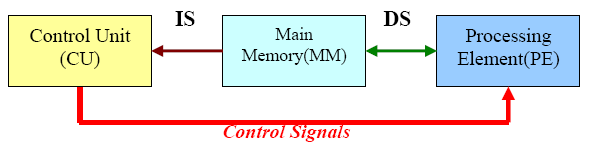
\includegraphics[width=10cm]{informatika/operacne_systemy_a_hw/obrazky/SISD.png}
  \end{center}

\item[Single Instruction, Multiple Data streams (SIMD)] -
    A computer which exploits multiple data streams against a single instruction stream to perform operations which may be naturally parallelized. For example, an array processor or GPU.
  \begin{center}
    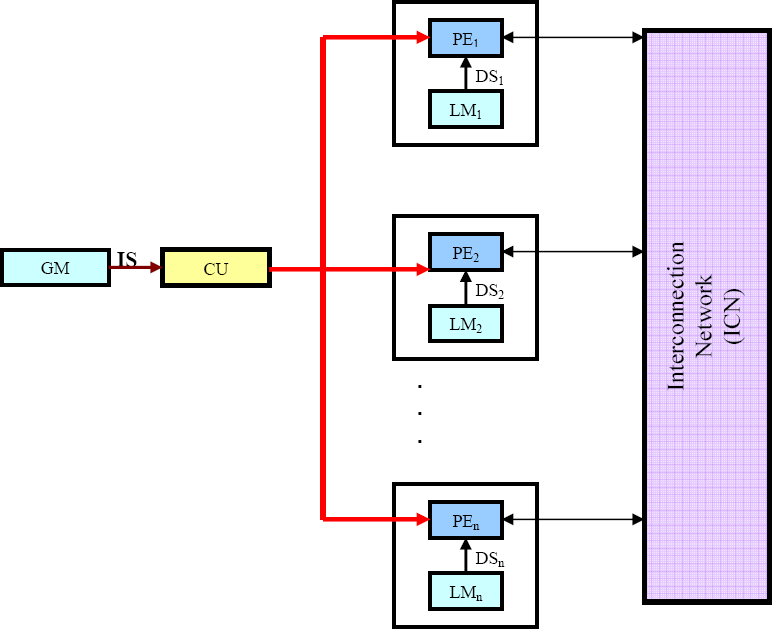
\includegraphics[width=12cm]{informatika/operacne_systemy_a_hw/obrazky/SIMD.png}
  \end{center}
  
\item[Multiple Instruction, Single Data stream (MISD)] -
    Multiple instructions operate on a single data stream. Uncommon architecture which is generally used for fault tolerance. Heterogeneous systems operate on the same data stream and must agree on the result. Examples include the Space Shuttle flight control computer.
  \begin{center}
    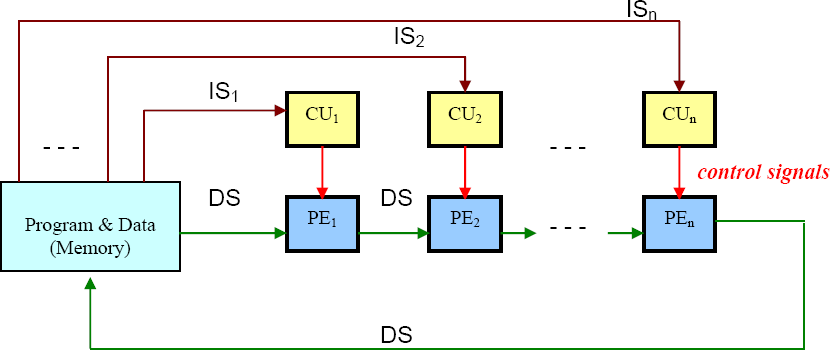
\includegraphics[width=12cm]{informatika/operacne_systemy_a_hw/obrazky/MISD.png}
  \end{center}
\item[Multiple Instruction, Multiple Data streams (MIMD)] -
    Multiple autonomous processors simultaneously executing different instructions on different data. Distributed systems are generally recognized to be MIMD architectures; either exploiting a single shared memory space or a distributed memory space. 

  \begin{center}
    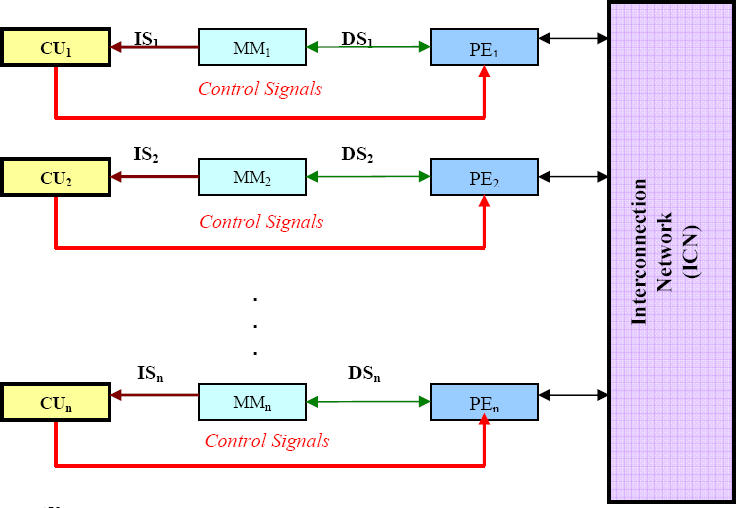
\includegraphics[width=12cm]{informatika/operacne_systemy_a_hw/obrazky/MIMD.png}
  \end{center}
\end{description}
\subsubsection*{Z�kladn� architektury po��ta��}

\begin{obecne}{Von Neumannova}
  \begin{pitemize}
      \item Po��ta� se skl�d� z ��d�c� jednotky, ALU, pam�ti a I/O jednotek
      \item �trukt�ra po��ta�a sa nemen� typom �lohy (tj. po��ta� je programovan� obsahem pam�ti). %to tuetschek sorry neumim cist... ajs
      \item Program se nejprve zavede do pam�ti, z n� se postupn� popo�ad� vyb�raj� instrukce (a n�sleduj�c� krok z�vis� na p�edchoz�m), po�ad� lze zm�nit instrukcemi skoku. 
      \item Do jedn� pam�ti, d�len� na bu�ky stejn� velikosti, se ukl�daj� i zpracov�van� data. Data jsou reprezentovan� bin�rn�. 
      \item V ka�d�m okam�iku je vykon�v�na jen jedna �innost. Je to architektura SISD (viz Flynnova taxonomie).
  \end{pitemize}

  Je pevn� dan� instruk�n� sada. Strojov� instrukce obsahuje opera�n� znak, kter� ur�uje druh operace, po�et parametr� atd., a operandov� ��st~-- um�stn�n� jednotliv�ch operand�. Vykonat jednu instrukci znamen�:
  \begin{pitemize}
          \item (fetch) na��ta� in�trukciu z pam�ti do procesoru
          \item (decode) zisti� o ak� in�trukciu ide
          \item (load) pripravi� zdrojov� operandy
          \item (execute) vykona� oper�ciu
          \item (store) ulozi� cie�ov� operandy
  \end{pitemize}

  P�i vykon�v�n� programu jsou pot�ebn� r�zn� registry~-- nejd�le�it�j�� jsou: PC (Program Counter, obsahuje adresu n�sleduj�c� instrukce), IR (Instruction Register, na�ten� instrukce pro zpracov�n� -- jm�no (typ) spolu s operandy (adresami)), SP (Stack Pointer, ukazatel na vrchol z�sobn�ku), MAR (memory access register~-- adresa do opera�n� pam�ti), MBR (memory buffer register, d�ta ��t�na/zapisov�na do pam�ti).

  Struktura jednoprocesorov�ho po��ta�e podle Von Neumanna:
  \begin{center}
    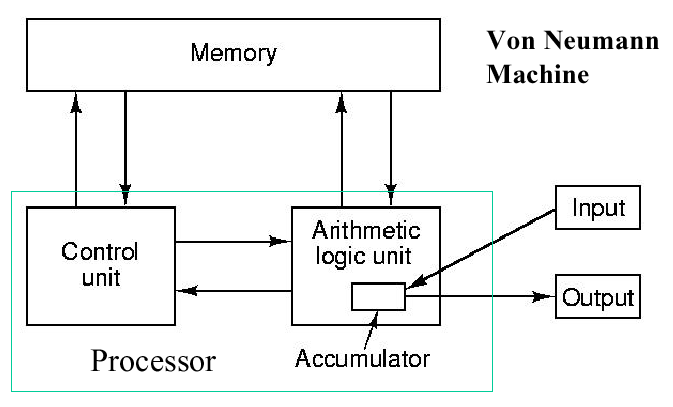
\includegraphics[width=8cm]{informatika/operacne_systemy_a_hw/obrazky/VonNeumann.png}
    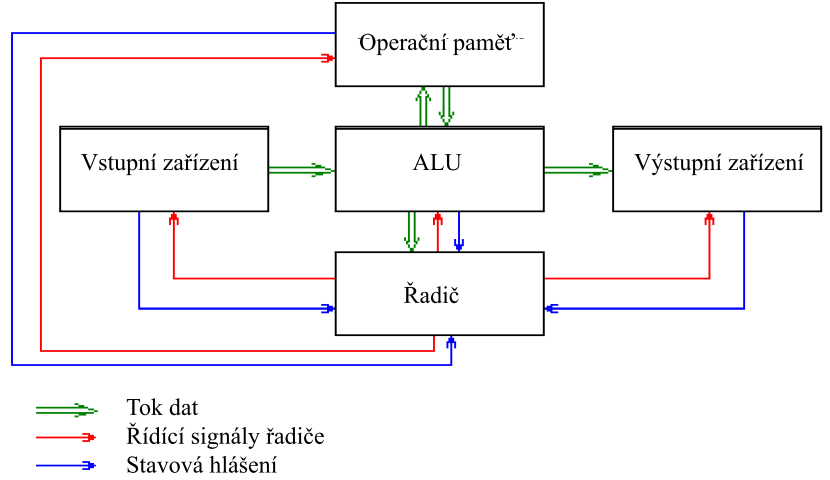
\includegraphics[width=8cm]{informatika/operacne_systemy_a_hw/obrazky/VonNeumann-Obdrzalek.png}
  \end{center}
\end{obecne}

\begin{description}
        \item[Control-flow]-- v�zna�n�m rysem von Neumannovy architektury je zp�sob prov�d�n�
programu. Strojov� instrukce, ze kter�ch se ka�d� p��mo spustiteln� program skl�d�, se prov�d�j� sekven�n�, jedna za druhou. Tedy ka�d� instrukce se provede tehdy, a� na ni dojde �ada, a nad takov�mi daty, jak� jsou pr�v� k dispozici. 
        \item[Data-flow (architektura ��zen� daty)]-- Alternativa k Control-flow. Okam�ik proveden� ur�it� akce se ��d� p�ipravenost� v�ech dat, kter� jsou k proveden� ur�it� akce zapot�eb�. V�hodou je mo�nost prov�d�t v�ce �innost� soub�n� - tedy v�t�� potenci�l paralelismu, kter� von Neumannov� koncepci naopak chyb�.
\end{description}

\begin{obecne}{Harvardsk�}
Vytvo�ena a� po Von Neumannov�, li�� se hlavn� t�m, �e program se ukl�d� do jin� pam�ti ne� data (tzn. jsou 2 \uv{druhy pam�ti}~-- instrukc� a dat). P��kladem jsou DSP procesory a mikrokontrolery. 

Nap�. AVR od Atmelu, a PIC~-- maj� pam� na program a data a RISC instruk�n� sadu; v�hoda odd�len�ch pam�t� je, �e m��ou m�t r�znou bitovou hloubku~-- 8 bitov� data, ale 12-, 14- �i 16- bitov� instrukce - nap�. ARM mus� ob�as pou��t v�ce ne� jednou instrukci na zpracov�n� obsahu pln� velikosti).

Oproti Von Neumannov� nehroz� nebezpe�� p�eps�n� programu sebou sam�m, ale kv�li v�t��mu po�tu pam�ov�ch sb�rnic je n�ro�n�j�� na v�robu. Pam� nav�c nelze d�lit podle pot�eby (rozd�len� je u� dan�).
\end{obecne}

\begin{e}{P��klad}{0}{Na�rtn�te typickou architekturu pocitace, ze kter� bude zrejm� um�st�n� a propojen� z�kladnich stavebn�ch prvku (procesor, pameti, radice a zar�zeni, sbenice). Ilustrujte na �rovni zakladnich krok� instrukcn�ho cyklu jak procesor vykon�v� program. Popi�te typy instrukci (a napi�te jejich p��klady), ze kter�ch se program z pohledu procesoru skl�d�.}
\\
  \textbf{Typick� (sb�rnicov�) architektura syst�mu:}
  \begin{center}
    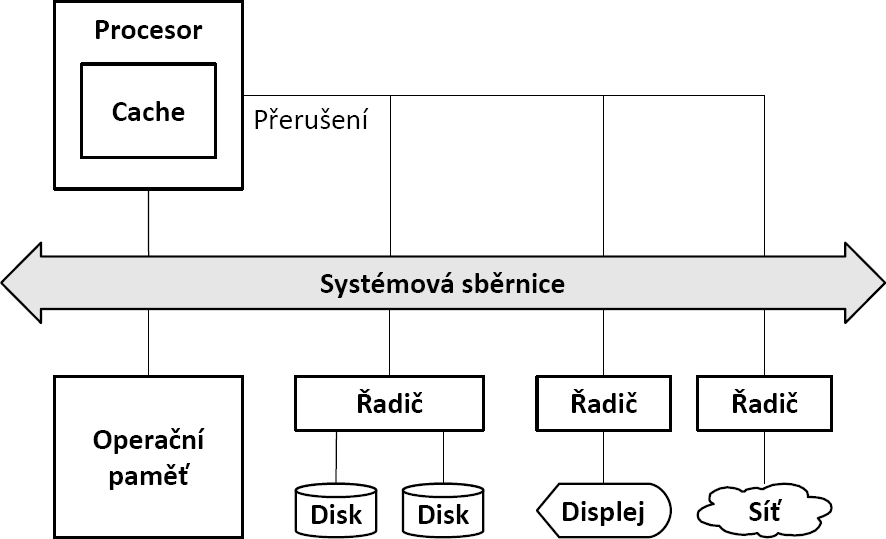
\includegraphics[width=8cm]{informatika/operacne_systemy_a_hw/obrazky/architektura.png}
  \end{center}

\textbf{Zpracov�n� instrukc�}
\begin{pitemize}
      \item \textbf{�ten�} instrukce z pam�ti na adrese v registru PC (program counter, obsahuje adresu n�sleduj�c� instrukce)
      \item \textbf{dek�dov�n�} instrukce a �ten� operand� z registr�
      \item \textbf{vykon�n�} operace odpov�daj�c� instruk�n�mu k�du (operace s obsahem registr�, v�po�et adresy a �ten�/z�pis do pam�ti, porovn�n� operand� pro podm�n�n� skok)
      \item \textbf{ulo�en�} v�sledku do registru (v�sledek operace s registry, data p�e�ten� z pam�ti)
      \item \textbf{posun} PC na n�sleduj�c� instrukci (n�sleduj�c� instrukce n�sleduje bezprost�edn� za pr�v� �tenou
instrukc�, pokud nen� �e�eno jinak - tzn. podm�n�n�/nepodm�n�n�
skok, v�jimka)       
  \end{pitemize} 

  \textbf{Typy instrukci (architektura MIPS):}
  \begin{pitemize}
      \item operace registr/registr, registr/immediate\footnote{operand (��slo) ulo�en�
      p��mo ve strojov�m k�du} (ALU operace, p�esun dat mezi registry)
      \item p�esuny dat registr/pam� (load/store architektura)
      \item podm�n�n� skoky (p�i rovnosti/nerovnosti obsahu dvou registr�)
      \item nepodm�n�n� skoky (v�etn� nep��m�ch skok� a skok� do podprogramu)
      \item speci�ln� instrukce (pr�ce se speci�ln�mi registry)
  \end{pitemize} 
\end{e}

\begin{e}{Start-up PC}{1}{zm��knu \uv{power on} a n�sleduje...}
\begin{penumerate}
    \item \emph{procesor} za�ne vykon�vat k�d (program) BIOSu (Basic Input/Output System)
    \item \emph{BIOS} zjist�, jak� HW je nainstalov�n, provede inicializaci grafick� karty a z (u�ivatelem definovan�ho) disku na�te a spust� boot sektor
    \item \emph{boot sektor} obsahuje k�d, kter� s pomoc� slu�eb BIOSu p�e�te z disku a spust� zavad�� OS
    \item \emph{zavad�� OS} p�e�te z disku k�d OS a spust� ho
    \item OS nastartuje syst�mov� slu�by a u�ivatelsk� rozhran�
\end{penumerate}
\end{e}

\begin{reportN}{Bulej}
Tenhle �lov�k se v tom vrtal hodn�, ale j� m�m tu v�hodu, �e jsem na st�edn� chodil na elektropr�myslovku, tak�e instrukc� a typ� instrukc� jsem mu tam popsal spoustu a i postup, jak procesor vykon�v� program, jsem v�d�l do detail� (a do detail� to cht�l). P�esv�d�il jsem ho asi hlavn� t�m, �e jsem odpov�dal takov�m t�m "samoz�ejm�m" zp�sobem ("a kdy� procesor vykon� instrukci, co d�l� d�l?" -"pokra�uje dal�� instrukc�" "no ale co p�esn� d�l�" -"no tenhle postup znovu, na�te dal�� instrukci..." "co to p�esn� znamen�?" -"no prost� zv�t�� instruction pointer o velikost pr�v� zpracovan� instrukce a t�m z�sk� adresu n�sleduj�c� instrukce, a opakuje tenhle postup").
\end{reportN}

\begin{reportN}{Peterka}
Peterka si narozdiel od Skopala aj precital to co som si napisal na papier. Popisal som tam Von Neumanna a Harvardsku architekturu (napisal som tam vsetko z vypiskov). K tomu nemal vyhrady. Potom vsak prisla horsia cast ked sa ma zacal vypytovat otazky typu: 

myslite si ze je dobre/zle ked moze byt prepisana ta pamat kde sa nachadza program, alebo ake su vyhody programovatelneho radica... dalej sa ma pytal na SISD,SIMD,MISD,MIMD, mal som mu nakreslit MISD ... co som moc nevedel... potom sa ma spytal na rozdiel Instruction flow control/Data flow control... dialog s Peterkom mi prisiel v niektorich castiach skor ako jeho monolog s mojim prikyvovanim hlavy...

Akorat jsem nebyl schopny si vzpomenout na architektury rizenou daty. A chtel vedet kolik radicu a ALU je potreba pri instrukcich SIMD,MIMD. Znamku nevim.

DATA FLOW + CONTROL FLOW (asi :)) podot�zka u mikroprocesor� a architektury 
\end{reportN}

\begin{reportN}{Peterka}
Von Neumannova architektura - dost temno
Harvardsk� Architektura - z�blesky
stroje ��zen� daty - brrr hr�za
tady u� ot�zky opravdu nev�m...
dod�m jen nepodce�te hardware - peterka d�v� v�dy jednu hardwarovou a jednu s�ovou ot�zku
dopl�uj�c�:
jak� jsou volac� konvence v Pascalu a C? viz zpracovan� ot�zky
co se stane kdy� zavol�me virtu�ln� fci p�ed vol�n�m konstruktoru? kone�n� jsem se chytil .)
\end{reportN}

\begin{reportN}{T�ma}
Za ferove povazujem ze vzal v uvahu ze som IOI a nedal mi konkretnu podotazku, skor tak prehladovo vsetko od architektur, cez procesory az po IO. Na druhej strane sa dost vrtal v zberniciach o ktorych som toho vedel pramalo ( myslim, ze v tych materialoch na statnice tam toho o nich moc nebolo ). Ked som zacal hovorit o preruseni, tak ma prerusil s tym, ze ak nechcem dopadnut ako kolega predo mnou ( patrne ho vyhodil ) tak nech som ticho
\end{reportN}

\subsection{Procesory, multiprocesory}

\begin{definiceN}{Procesor} 
Procesor (CPU – central processing unit) je ústřední výkonnou jednotkou počítače, která čte z paměti instrukce a na jejich základě vykonává program.

Základnými súčasťami procesora sú:
\begin{pitemize}
	\item řadič nebo řídicí jednotka, která řídí tok programu, tj. načítání instrukcí, jejich dekódování, načítání operandů instrukcí z operační paměti a ukládání výsledků zpracování instrukcí
	\item sada registrů k uchování operandů a mezivýsledků.
	\item jedna nebo více aritmeticko-logických jednotek (ALU), které provádí s daty aritmetické a logické operace.
	\item některé procesory obsahují jednu nebo několik jednotek plovoucí čárky (FPU), které provádí operace v plovoucí řádové čárce.
\end{pitemize}
\end{definiceN}

\begin{poznamka}
Súčasné procesory navyše často obsahujú ďalšie rozsiahle funkčné bloky (cache, rôzne periférie)~-- ktoré z \uv{ortodoxného hladiska} nie sú priamo súčasťou \emph{jadra procesoru}. Niektoré procesory môžu obsahovať viac jadier (+logiku slúžiacu k ich vzájomnému prepojeniu). Ďalším trendom je SoC (System on Chip), kde sa na čipe procesora nachádzajú aj ďalšie subsystémy napr. na spracovanie zvuku, grafiky alebo pripojenie externých periférií (takéto riešenia sa využívajú väčšinou v PDA, domácej elektronike, mobiloch atď.).
\end{poznamka}

\begin{obecne}{Dělení podle instruční sady}
Podľa inštrukčnej sady je možné procesory rozdeliť na:
\begin{pitemize}
	\item \textbf{CISC} (Complex Instruction Set Computer): poskytuje rozsiahlu inštrukčnú sadu spolu s rôznymi variantami inštrukcií. Jedna inštrukcia napr. môže vykonať veľa low-level operácií (načítanie z pamäti, vykonať aritmetickú operáciu a výsledok uložiť). Takéto inštrukcie zjednodušovali zápis programov (inštrukcie boli bližšie vyšším programovacím jazykom) a zmenšovali veľkosť programu a počet prístupov do pamäti~-- čo bolo v 60tych rokoch dôležité. Avšak nie vždy je vykonanie jednej zložitej operácie rýchlejšie ako vykonanie viac menej zložitých miesto toho (napr. kvôli zložitému dekódovaniu a použitiu mikrokódu na volanie jednoduchých \uv{podinštrukcií}). Príkladmi CISC architektúr procesorov sú System/360, Motorola 68000 a Intel x86. V súčasnosti napr. x86 rozkladá zložité inštrukcie na \uv{micro-operations} ktoré môžu byť pipeline-ou spracované paralelne a vyšší výkon je tak dosahovaný na väčšom rozsahu inštrukcií. Vďaka tomu sú súčasné x86 procesory minimálne rovnako výkonné ako ozajstné RISC architektúry.
	\item \textbf{RISC} (Reduced Instruction Set Computer): design CPU ktorý uprednosňuje jednoduchšiu inštrukčnú sadu a menšiu zložitosť adresovacích modelov~-- vďaka čomu je možné dosiahnuť lacnejšiu implementáciu, väčšiu úroveň paralelizmu a účinnejšie kompilátory. Dôvodom vzniku bolo aj nevyužívanie celej CISC inštrukčnej sady a upredňostňovania len obmedzenej podmnožiny (designéri procesorov potom optimalizovali len tieto podmnožiny a tak sa zvyšné inštrukcie používali ešte menej...). Kvôli väčšiemu počtu inštrukcií však musia RISC procesory častejšie pristupovať k pamäti... Príkladmi RISC procesorov sú napr. SPARC a ARM. V architekturách typu \textbf{Post-RISC} jde o spojení RISCových vlastností s technikami zvýšení výkonu, jako je out-of-order vykonávání a paralelismus.
    \item \textbf{VLIW}: Very Long Instruction Word or VLIW refers to a CPU architecture designed to take advantage of instruction level parallelism (ILP). A processor that executes every instruction one after the other (i.e. a non-pipelined scalar architecture) may use processor resources inefficiently, potentially leading to poor performance. The performance can be improved by executing different sub-steps of sequential instructions simultaneously (this is pipelining), or even executing multiple instructions entirely simultaneously as in superscalar architectures. The VLIW approach, on the other hand, executes operation in parallel based on a fixed schedule determined when programs are compiled. Since determining the order of execution of operations (including which operations can execute simultaneously) is handled by the compiler, the processor does not need the scheduling hardware that the three techniques described above require. As a result, VLIW CPUs offer significant computational power with less hardware complexity (but greater compiler complexity) than is associated with most superscalar CPUs.
    \item \textbf{EPIC}: (Někdy označován za poddruh VLIW) Explicitly Parallel Instruction Computing (EPIC) is a computing paradigm that began to be researched in the 1990s. This paradigm is also called Independence architectures. It was used by Intel and HP in the development of Intel’s IA-64 architecture, and has been implemented in Intel’s Itanium and Itanium 2 line of server processors. The goal of EPIC was to increase the ability of microprocessors to execute software instructions in parallel, by using the compiler, rather than complex on-die circuitry, to identify and leverage opportunities for parallel execution. This would allow performance to be scaled more rapidly in future processor designs, without resorting to ever-higher clock frequencies, which have since become problematic due to associated power and cooling issues.
\end{pitemize}
\medskip
TODO: asi opravit, možná zpřesnit VLIW a EPIC a určitě přeložit

\medskip
Řekneme, že procesor má \emph{ortogonální instrukční sadu}, pokud žádná instrukce nepředpokládá implicitně použití některých registrů. To umožňuje jednodušší práci algoritmům přidělování registrů v překladačích. Příkladem neortogonální instrukční sady je i x86.
\end{obecne}

\begin{obecne}{Další dělení}
Ďalej je možné procesory rozdeliť podľa dĺžky operandov v bitoch (8, 16, 32, 64...), ktorý je procesor schopný spracovať v jednom kroku. V embedded zariadeniach sa najčastejšie používajú 4- a 8-bitové procesory. V PDA, mobiloch a videohrách 8 resp. 16 bitové. 32 a viac bitov využíajú napr. osobné počítače a laserové tlačiarne.

Dôležitou vlastnosťou je aj taktovacia frekvencia jadra, MIPS (millions of instructions per second) a jeho rýchlosť. V súčasnosti je ťažké dávať do súvislosti výkon procesorov s ich frekvenciou (resp. MIPS)~-- kým Pentium zvládne na výpočet vo floatoch, jednoduchý 8-bitový PIC na to potrebuje oveľa viac taktov. Ďalším \uv{problémom} je superskalarita procesorov, ktorá im umožňuje vykonať viacero nezávislých inštrukcií počas jedného taktu.
\end{obecne}

\begin{obecne}{Techniky pro zvýšení výkonu}
Zvyšovať výkon (procesorov) je možné viacerými spôsobmi. Najjednoduchším (a najpomalším) typom je Subskalárny CPU (načíta a spracúva len jednu inštrukciu naraz~-- preto musí celý procesor čakať kým vykonávanie inštrukcie skončí; je tak zdržovaný dlhšie trvajúcimi inštrukciami). 

\begin{center}
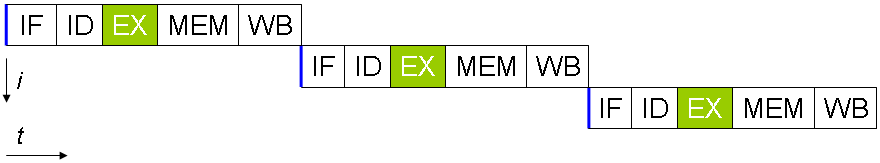
\includegraphics[width=8cm]{informatika/operacne_systemy_a_hw/obrazky/Nopipeline.png}
\end{center}

Pokusy o dosiahnutie skalárneho a lepšieho výkonu vyústili do designov ktoré sa správajú menej lineárne a viac paralelne. Čo sa týka paralelizmu v procesoroch, používajú sa dva druhy pojmov na ich klasifikáciu~-- \emph{Instruction level parallelism} (zvyšovanie rýchlosti vykonávania inštrukcií v procesore a teda zväčšovanie využitia prostriedkov na čipe) a \emph{Thread level parallelism} (zväčšovanie počtu vlákien, ktoré dokáže CPU vykonávať naraz).
\begin{pitemize}
  \item \textbf{pipeline}: 
  Zlepšenie je možné dosiahnúť pomocou \uv{instruction pipelining}-u, ktoré je použíté vo väčšine moderných procesorov. Umožňuje vykonanie viac ako jednej inštrukcie v jednom kroku vďaka rozloženiu spracovávania inštrukcie na viac menších krokov: 
  \begin{center}
  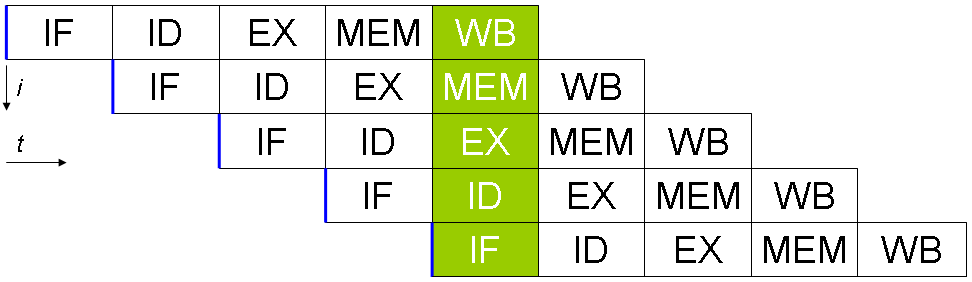
\includegraphics[width=8cm]{informatika/operacne_systemy_a_hw/obrazky/Fivestagespipeline.png}
  \end{center}

  \item \textbf{superskalarita}: Dialša možnosť je použitie superscalar designu, ktorý obsahuje dlhú inštrukčnú pipeline a viacero identických execution jednotiek.  
  \begin{center}
  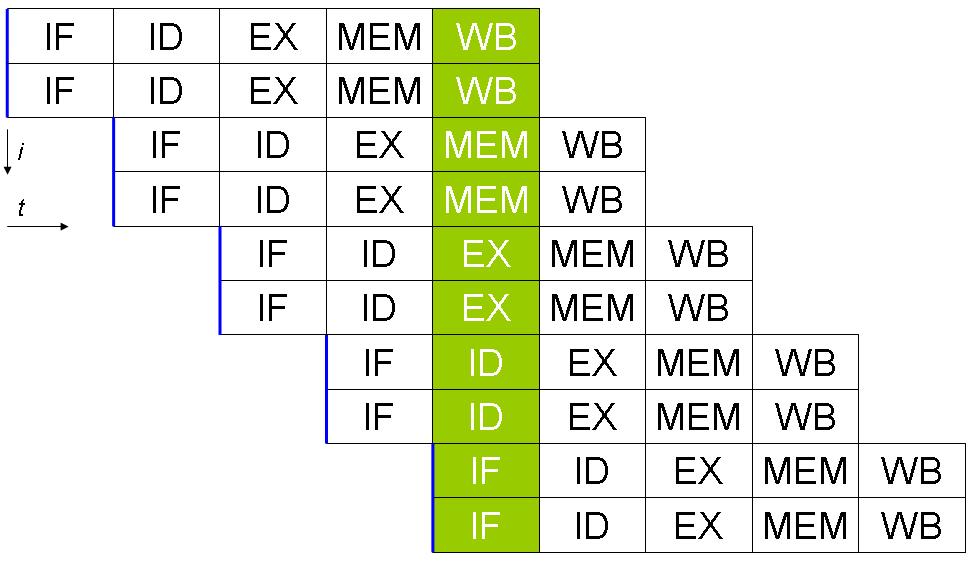
\includegraphics[width=8cm]{informatika/operacne_systemy_a_hw/obrazky/Superscalarpipeline.png}
  \end{center}	

  \item \textbf{Out of order execution}
  \begin{penumerate}
	  \item Načtení instrukce, případně její rozdrobení na mikroinstrukce
	  \item Zařazení do vyčkávací stanice (instruction pool)
	  \item Instrukce čeká na všechny svoje operandy
	  \item Instrukce se vykoná ve své výkonné jednotce (je vybírána z instruction poolu nezávisle na ostatních)
	  \item Výsledky se uchovají ve frontě (reorder buffer)
	  \item Až se všechny starší instrukce zapíší do registrů, zapíše se výsledek této instrukce (opětovné řazení)
  \end{penumerate}

  \item \textbf{Predikce skoků}~-- hluboké pipeliny mají problém, pokud podmíněný skok není proveden; dynamická predicke skoků (historie CPU~-- vzory nějaké hloubky) vs. statická (bez nápovědy~-- skok vpřed se neprovede, skok vzad se provede; s nápovědou~-- překladač odhaduje pravděpodobnost skoku)

  \item \textbf{Spekulativní vykonávaní}~-- vykonávání kódu, který nemusí být zapotřebí; významná disproporce mezi rychlostí CPU a paměti; typické využití je značné předsunutí čtecích operací; CPU provádí i odsouvání zápisových operací


  \item \textbf{Data parallelism}: SIMD inštrukcie (napr. multimediálne inštrukcie), vektorové procesory...
\end{pitemize}
\end{obecne}

\subsubsection*{Multiprocesory}

TODO: jde o copy \& paste z Wiki ... předělat česky/slovensky
\medskip

\begin{definiceN}{Multiprocesor}
  O \emph{multiprocesoru} mluvíme, pokud je použito dvou nebo více procesorů
  (CPU) v rámci jednoho počítačového systému. Termín je také používán mluvíme-li
  o schopnosti systému využívat více procesorů a/nebo schopnosti rozdělovat
  úlohy mezi jednotlivými procesory.
\end{definiceN}

\begin{obecne}{Vztah k datům a instrukcím}
In multiprocessing, the processors can be used to execute a single sequence of instructions in multiple contexts (single-instruction, multiple-data or SIMD, often used in vector processing), multiple sequences of instructions in a single context (multiple-instruction, single-data or MISD, used for redundancy in fail-safe systems and sometimes applied to describe pipelined processors or hyperthreading), or multiple sequences of instructions in multiple contexts (multiple-instruction, multiple-data or MIMD).
\end{obecne}

\begin{obecne}{Symetrie}
In a multiprocessing system, all CPUs may be equal, or some may be reserved for special purposes. A combination of hardware and operating-system software design considerations determine the symmetry (or lack thereof) in a given system. For example, hardware or software considerations may require that only one CPU respond to all hardware interrupts, whereas all other work in the system may be distributed equally among CPUs; or execution of kernel-mode code may be restricted to only one processor (either a specific processor, or only one processor at a time), whereas user-mode code may be executed in any combination of processors. Multiprocessing systems are often easier to design if such restrictions are imposed, but they tend to be less efficient than systems in which all CPUs are utilized equally.

Systems that treat all CPUs equally are called symmetric multiprocessing (SMP) systems. In systems where all CPUs are not equal, system resources may be divided in a number of ways, including asymmetric multiprocessing (ASMP), non-uniform memory access (NUMA) multiprocessing, and clustered multiprocessing (qq.v.).
\end{obecne}

\begin{obecne}{Těsnost spojení multiprocesorů}
\begin{pitemize}
    \item \textbf{Tightly-coupled} multiprocessor systems contain multiple CPUs that are connected at the bus level. These CPUs may have access to a central shared memory (SMP or UMA), or may participate in a memory hierarchy with both local and shared memory (NUMA). The IBM p690 Regatta is an example of a high end SMP system. Intel Xeon processors dominated the multiprocessor market for business PCs and were the only x86 option till the release of AMD's Opteron range of processors in 2004. Both ranges of processors had their own onboard cache but provided access to shared memory; the Xeon processors via a common pipe and the Opteron processors via independent pathways to the system RAM.

    \item \textbf{Chip multiprocessors}, also known as multi-core computing, involves more than one processor placed on a single chip and can be thought of the most extreme form of tightly-coupled multiprocessing. Mainframe systems with multiple processors are often tightly-coupled.

    \item \textbf{Loosely-coupled multiprocessor} systems (often referred to as clusters) are based on multiple standalone single or dual processor commodity computers interconnected via a high speed communication system (Gigabit Ethernet is common). A Linux Beowulf cluster is an example of a loosely-coupled system.
\end{pitemize}
Tightly-coupled systems perform better and are physically smaller than loosely-coupled systems, but have historically required greater initial investments and may depreciate rapidly; nodes in a loosely-coupled system are usually inexpensive commodity computers and can be recycled as independent machines upon retirement from the cluster.

\textbf{SMP} (Symmetric Multiprocessing): viac procesorov so zdieľanou operačnou pamäťou (nutné mechanizmy na zabránenie nesprávnych náhľadov na pamäť a migráciu procesov medzi procesormi). SMP systems allow any processor to work on any task no matter where the data for that task are located in memory; with proper operating system support, SMP systems can easily move tasks between processors to balance the workload efficiently.
\end{obecne}

\subsection{Sb�rnice, protokoly}

\begin{pitemize}
	\item \textbf{Struktura sb�rnice}: datov� linky, adresov� linky, ��d�c� linky
	\item \textbf{Synchronn� p�enos} (vznik ud�losti je d�n hodinov�m sign�lem) vs. \textbf{asynchronn� p�enos} (vznik ud�losti je ur�en p�edch�zej�c� ud�lost�~-- napr. signaliz�ciou za�iatku d�t) 
	\item \textbf{Parametry sb�rnice}: 
	\begin{pitemize}
	  \item \emph{datov� ���ka}~-- po�et p�en�en�ch bit� v jednom okam�iku,
	  \item \emph{kapacita}~-- po�et bit� p�enesen�ch za �as,
	  \item \emph{rychlost}~-- kapacita sb�rnice normovan� k jednotce informace. 
	\end{pitemize}  
	\item \textbf{��zen� po�adavk�}: 
	\begin{pitemize}
	  \item \emph{centr�ln�}~-- n�hodn�, dle po�ad� vzniku po�adavk�, prioritn�,
	  \item \emph{distribuovan�}~-- kolizn� (CSMA/CD), token bus, prioritn� linka (daisy chain).
	\end{pitemize} 
	\item \textbf{P�enos dat po sb�rnici} m��e prob�hat bu� za ��asti procesoru (zdroj $\rightarrow$ CPU $\rightarrow$ c�l), nebo bez. Bez procesoru to m��e b�t nap�.:
	\begin{pitemize}
		\item d�vkov� re�im~-- domluva mezi CPU a �adi�em na dob� obsazen� sb�rnice (napr. pomocou zdvihnutia \uv{lock flagu} na zbernici)
		\item kraden� cykl�~-- �adi� na dobu p�enosu \uv{usp�} procesor (nelze uspat na dlouho, je to technicky n�ro�n�j��)
		\item transparentn� re�im~-- �adi� rozezn�, kdy procesor nepou��v� sb�rnici, obvykle nelze v�t�� p�enosy najednou
		\item DMA (Direct Memory Access)~-- speci�ln� jednotka pro prov�d�n� p�enos� dat (mezi za��zen�mi a pam�t�)
	\end{pitemize}
	Jednou z technik, pou��van�ch k p�enosu dat po sb�rnici �adi�i DMA, je \emph{scatter-gather}. Znamen� to, �e v r�mci jednoho p�enosu se zpracov�v� v�c ne nutn� souvisl�ch blok� dat. 
	\begin{pitemize}
	    \item \emph{scatter}~-- DMA �adi� v r�mci 1 p�enosu ulo�� z 1 m�sta data na n�kolik r�zn�ch m�st (nap� hlavi�ky TCP/IP - jinak zbyte�n� kop�rov�n�)  
	    \item \emph{gather}~-- nap�. p�i str�nkov�n� pam�ti - na��t�n� str�nek, kter� fyzicky na disku nemus� b�t u sebe, slo�en� na 1 m�sto do pam�ti.
	\end{pitemize}
\end{pitemize}

P��klady sb�rnic:
\begin{pitemize}
	\item ISA, EISA
	\item ATA, ATAPI~-- UltraDMA, Serial-ATA (SATA)
	\item SCSI (Small Computer System Interface)
	\item PCI, PCI-X, PCI Express
	\item AGP (Advanced Graphics Port)
	\item USB (Universal Serial Bus)
	\item FireWire (IEEE 1394)
	\item RS485
	\item $I^{2}C$
\end{pitemize}

P��buzn� sb�rnic:
\begin{pitemize}
	\item IrDA
	\item Bluetooth
	\item Wi-Fi, WiMAX 
\end{pitemize}

\subsection{Vstupn� a v�stupn� za��zen�, ukl�d�n� a p�enos dat}

Za��zen� maj� r�zn� charakteristiky:
\begin{pitemize}
    \item \textbf{druh}~-- blokov� (disk, s�ov� karta), znakov� (kl�vesnice, my�)
    \item \textbf{p��stup}~-- sekven�n� (datov� p�ska), n�hodn� (hdd, cd)
    \item \textbf{komunikace}~-- synchronn� (pracuje s daty na ��dost~-- disk), asynchronn� (\uv{nevy��dan�} data~-- s�ov� karta)
    \item \textbf{sd�len�}~-- sd�len� (preemptivn�, lze odebrat~-- s�ov� karta (po multiplexu OS)), vyhrazen� (nepreemptivn�~-- tisk�rna, sd�len� se realizuje p�es \textbf{spooling} - frontou). Re�ln� se rozd�ly st�raj�.
    \item \textbf{rychlost} (od n�kolika Bps po GBps)
    \item \textbf{sm�r dat}~-- R/W, R/O (CD-ROM), W/O (tisk�rna) 
\end{pitemize}

\begin{e}{Propojovac� syst�my}{0}{0}
D�l� se na \textbf{dvoubodov� spoje} (vztah 1:1), jde nap�. o p��m� spojen� porty, k��ov� p�ep�na�, kde nen� nutn� ��dn� adresace. Druhou mo�nost� jsou \textbf{v�cebodov� spoje}, kde v�ce ��astn�k� sd�l� p�enosov� m�dium jako nap�. sb�rnice nebo p�i broadcastingu.
\end{e}

\textbf{Procesor} m��e p�istupovat k I/O za��zen�m dv�ma zp�soby:
\begin{pitemize}
    \item \textbf{port-mapped I/O} -- speci�ln� adresov� port CPU, kter� m� i speci�ln� instrukce pro pr�ci (IN, OUT) s I/O za��zen�m, kter� tak� maj� vlastn� adresov� prostor (bu� p��mo vlastn� sb�rnici, nebo extra I/O pinem), d�ky tomu se tak� ��k� \uv{isolated I/O},
    \item \textbf{memory-mapped I/O} -- pam�ov� mapov�n�, kter� mapuje I/O za��zen� p��mo do adresov�ho prostoru fyzick� pam�ti. Tato ��st adresov�ho prostoru m��e b�t vyhrazen� trvale nebo i jen do�asn�. Za��zen� poslouch� na adresov� sb�rnici, aby v�d�lo, kdy m� pracovat (odpov�dat, ...).
\end{pitemize}

  \begin{center}
    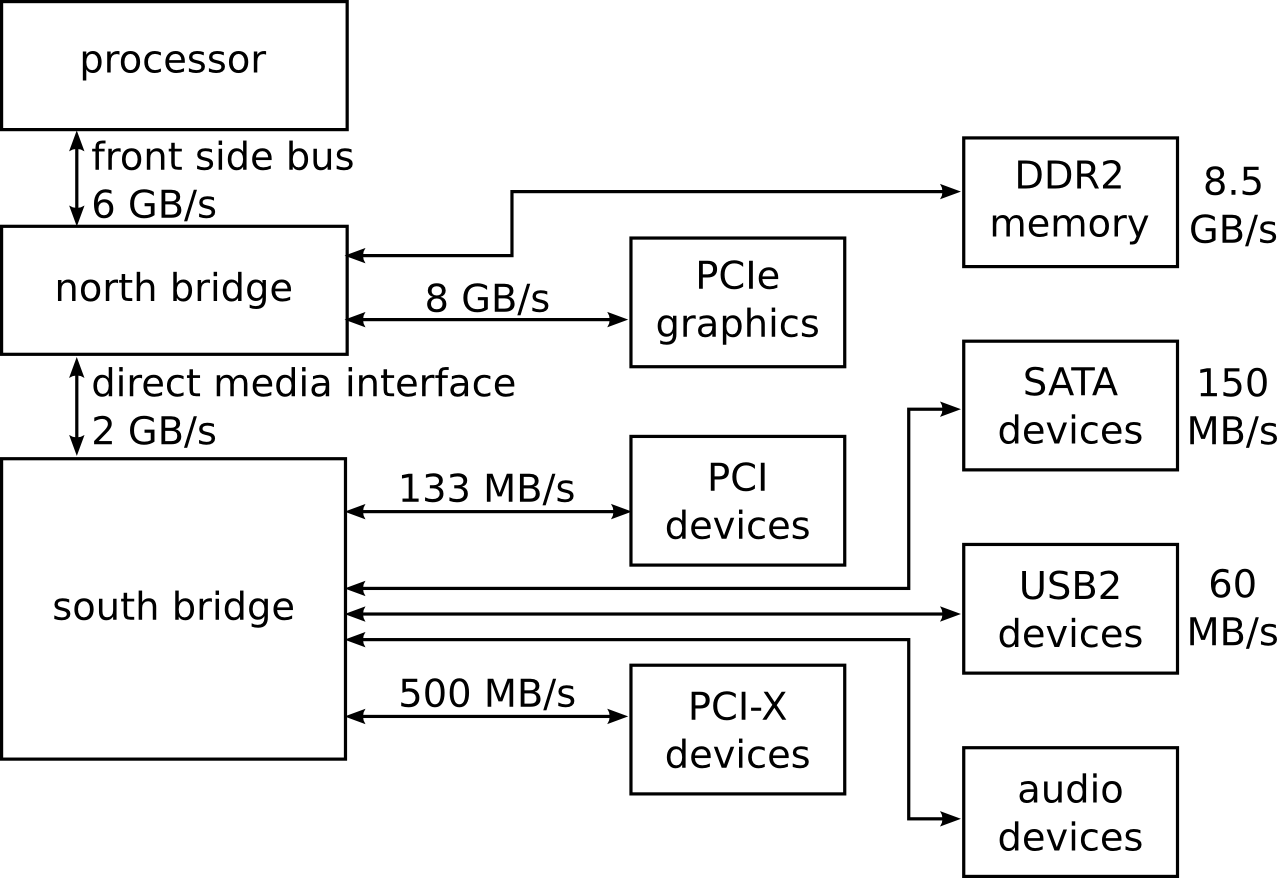
\includegraphics[width=8cm]{informatika/operacne_systemy_a_hw/obrazky/bus_north_south_bridge.png}
  \end{center}

\begin{e}{Sb�rnice}{0}{0}
Sb�rnice je sada vodi�� propojuj�c� v�ce za��zen�. Vodi�e jsou odd�len� pro ��zen� (po�adavky, potvrzen�, typ dat) a data (p�enos dat, adresov�n�). V�hodou je univerz�lnost a n�zk� cena, nev�hodami pak omezen� d�lkou a dan� v d�sledku pou��v�n� rozmanit�ch za��zen�, tak� potenci�ln� \uv{bottleneck}.\\
Transakce na sb�rnici za��n� po�adavkem (vysl�n� p��kazu a adresy c�le), na kter� mus� c�l odpov�d�t potvrzen�m, na�e� n�sleduje p�enos dat mezi ��astn�ky \textbf{master/initiator} (kte�� pos�laj� po�adavek) a \textbf{slave/target}, kte�� pos�laj�/p�ij�maj� data.\\
\textbf{��zen�} -- \textbf{synchronn�} (podle hodin, jednodu���, rychlej��, ale omezen� d�lka sb�rnice a stejn� �as v�em) vs. \textbf{asynchronn�} (obecn�j��, slo�it�j��, zato bez omezen� d�lky, ale s ni��� rychlost�, nap�. USB, FireWire)\\
\textbf{p�id�lov�n�} -- \textbf{centralizovan�} (master ��d� a �ek� na p�id�len�, kter� p�id�luje arbitr podle priority a fairness, master po proveden� operace d� arbitrovi v�d�t, �e je sb�rnice op�t voln�) vs. \textbf{distribuovan�}, kter� m��e b�t kolizn� nebo zalo�en� na \uv{samov�b�ru}.
\end{e}

\begin{figure}[h]
  \centering
  \subfloat[polling]{\label{fig:bus_polling}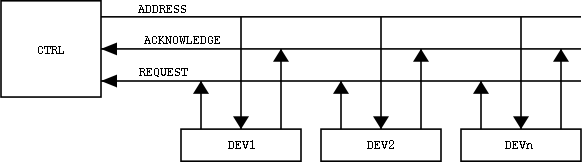
\includegraphics[width=0.49\textwidth]{informatika/operacne_systemy_a_hw/obrazky/bus_polling.png}} \hfill
  \subfloat[prioritn� z�et�zen�, daisy chain]{\label{fig:bus_daisy_chain}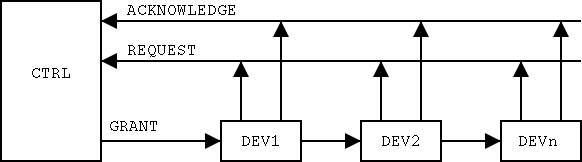
\includegraphics[width=0.49\textwidth]{informatika/operacne_systemy_a_hw/obrazky/bus_daisy_chain.png}} \hfill
  \subfloat[nez�visl� ��dosti]{\label{fig:bus_independent}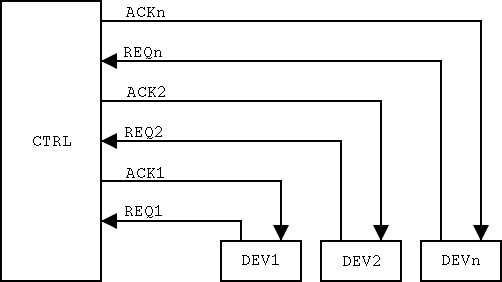
\includegraphics[width=7cm]{informatika/operacne_systemy_a_hw/obrazky/bus_independent.png}}
    \caption{centralizovan� p�id�lov�n�}
  \label{fig:bus_centralizovane_pridelovani}
\end{figure}
Informace o stavu za��zen� m��e CPU z�sk�vat:
\begin{pitemize}
    \item \textbf{polling}~-- aktivn� �ek�n� na zm�nu za��zen� (program periodicky kontroluje stav), pro pomal� za��zen� vznik� zna�n� re�ie
    \item \textbf{interrupt-driven I/O}~-- asynchronn� p�eru�en� od za��zen�, kter� samo signalizuje zm�nu stavu, na co� reaguje obslu�n� rutina. CPU ov�em nen� na p�eru�en� p�ipraven, tak mus� ulo�it stav programu $\rightarrow$ stoj� to �as. CPU mus� podporovat tuto signalizaci p�eru�en�, identifikovat zdroj p�eru�en�, vybrat spr�vnou obslu�nou rutinu. Syst�m mus� zajistit doru�en� p�eru�en� k CPU a d�le �adi� jejich podle priority ur�� jejich po�ad� (m��e jich b�t v�ce ne� m� CPU vstup�). Pr�b�h:
    \begin{penumerate}
    \item     Vn�j�� za��zen� vyvol� po�adavek o p�eru�en�
    \item			I/O rozhran� vy�le sign�l IRQ na �adi� p�eru�en� (na port IRQ 2)
    \item     �adi� p�eru�en� vygeneruje sign�l INTR � �n�kdo� ��d� o p�eru�en� a vy�le ho k procesoru.
    \item     Procesor se na z�klad� maskov�n� rozhodne obslou�it p�eru�en� a sign�lem INTA se zept�, jak� za��zen� ��d� o p�eru�en�.
    \item     �adi� p�eru�en� identifikuje za��zen�, kter� ��d� o p�eru�en� a ode�le ��slo typu p�eru�en� k procesoru
    \item     Procesor ulo�� stavov� informace o pr�v� zpracov�van�m programu do z�sobn�ku.
    \item     Podle ��sla typu p��choz�ho p�eru�en� nalezne ve vektoru p�eru�en� adresu p��slu�n�ho obslu�n�ho podprogramu.
    \item     Vyhled� obslu�n� podprogram obsluhy p�eru�en� v pam�ti a vykon� ho.
    \item     Po proveden� obslu�n�ho programu op�t obnov� ulo�en� stavov� informace ze z�sobn�ku a p�eru�en� program pokra�uje d�l.
\end{penumerate}
    
\end{pitemize}

P�enos dat mezi za��zen�m a CPU/pam�t�:
\begin{penumerate}
    \item \textbf{PIO (Programmed I/O)}~-- data p�en�ena za ��asti CPU (pln� zam�stn�n), p�enos realizov�n cyklem v programu, rychl� p�enos, ale neefektivn� vyu�it� CPU, pak p�i�lo DMA
    \item \textbf{DMA (Direct Memory Access)}~-- za��zen� si samo ��d� p��stup na sb�rnici a p�en�� data z/do pam�ti bez ��asti CPU; po skon�en� p�enosu p�eru�en� (ozn�men� o dokon�en�) nap�, p�enos dat mezi HDD a RAM
\end{penumerate}

\begin{e}{Bus mastering}{0}{0}
Slou�� pro p�enos dat mezi za��zen�m a pam�t� nebo mezi dv�ma za��zen�mi. Jde o to, �e sb�rnici m��e ��dit (za��t transakci, b�t masterem) libovoln� ��astn�k (CPU vn�m�n jako jeden z nich), st�le je nutn� p�enos \emph{nastavit} z programu.
\end{e}

\subsubsection*{DMA}
CPU nastav� p�enos a nech� DMA pracovat, a� je operace dokon�ena, po�le se p�eru�en�, tedy mezit�m m��e CPU pracovat jinde. DMA �adi� je obvod pro ��zen� p�enos� na sb�rnici mezi pam�t� a za��zen�mi nebo i pouze v pam�ti. U multiprocesor� se u��v� i k p�enosu dat mezi j�dry. D�le b�n� u pevn�ch disk�, grafick�ch, zvukov�ch a s�ov�ch karet. DMA �adi� obsahuje registry, do kter�ch m��e CPU zapisovat nastaven� p�enosu (adresa v pam�ti, po�et byt�, sm�r r/w, jak� za��zen�) -- tomu se ��k� \textbf{burst mode}, ve kter�m vysta�� jeden adresov� cyklus na cel� blok dat. D�le se vyu��v� p�i p�enosu dat do/z v�ce nesouvisl�ch buffer� (\textbf{scatter/gather}, tak� vektorov� I/O).

\begin{e}{Pr�ce �adi�e DMA}{0}{0}
\begin{pitemize}
    \item generuje adresy pam�ti a periferie, generuje ��d�c� sign�ly pro �ten�/z�pis
    \item generuje sign�ly pro procesor, aby zajistil, �e procesor nep�istupuje (nezapisuje) na sb�rnici
    \item �adi� s�m se chov� jako periferie
    \item program nastavuje parametry p�enosu, tj. odkud se bude p�en�et, kam, a kolik (2 ��ta�e, kan�l DMA)
    \item za��zen� p�ipojena na kan�l DMA, p�i p�enosu je c�lov� za��zen� aktivov�no �adi�em, nikoliv vystaven�m adresy   
\end{pitemize}
\end{e}

\begin{e}{Posloupnost ud�lost�}{0}{0}
��sla p�ed ud�lost� odpov�daj� ��sl�m na obr�zku n�e.
\begin{pitemize}
    \item program nastav� �adi� a periferii a povol� p�enos
    \item[(1)] aktivac� sign�lu DREQx periferie po��d� �adi� DMA o p�enos slova z/do pam�ti
    \item �adi� DMA zkontroluje nastaven� kan�lu vyhodnot� prioritu ��dosti
    \item[(2)] aktivac� sign�lu HOLD �adi� DMA po��d� CPU o p�id�len� sb�rnice
    \item[(3)] pokud CPU nepot�ebuje sb�rnici, odpoj� se od sb�rnice a signalizuje HLDA
      \subitem - CPU po��d testuje HOLD na za��tku strojov�ho cyklu
    \item[(4)] po p�ijet� HLDA �adi� p�iprav� sb�rnici pro p�enos
    \subitem - vystav� adresu v pam�ti a ��d�c� sign�ly pro �ten�/z�pis z/do pam�ti/periferie
    \item[(5)] �adi� DMA aktivuje sign�l DACKx, kter�m vyzve periferii k vystaven�/p�e�ten� dat na/ze sb�rnice
    \item[(7)] v z�vislosti na re�imu bu� p�enos kon��, nebo pokra�uje dal��m slovem dokud je DREQx aktivn�
    \item p�i posledn�m slov� �adi� aktivuje sign�l EOP
    \item[(8)] p�i ukon�en� p�enosu �adi� uvoln� sign�l HOLD
    \item[(9)] procesor uvoln� HLDA a p�ipoj� se ke sb�rnici
\end{pitemize}
\begin{figure}[h]
  \centering
  \label{fig:dma_block_transfer}
  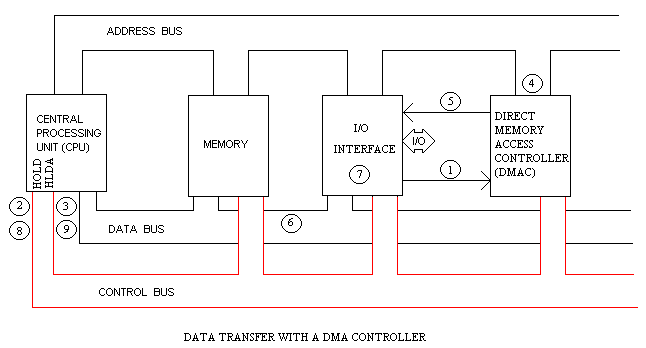
\includegraphics[width=17cm]{informatika/operacne_systemy_a_hw/obrazky/dma_block_transfer.png}
%  \caption{DMA burst mode}
\end{figure}
\end{e}

Probl�my u DMA spo��vaj� v odst�n�n� CPU od pam�ti, co� m��e vyvolat \textbf{pam�ovou koherenci}, slu�n� �e�eno pomoc� DMA obejdeme cache CPU, kde mohou b�t aktu�ln�j�� hodnoty ne� v pam�ti, a tud� m�me probl�m Houstone. �e�� se to t�m, �e procesor sleduje, na jak� adresy se p�istupuje a pokud tam padne n�jak�, kterou m� v cache, tak to za�ne �e�it.

\begin{figure}[h]
  \centering
  \label{fig:dma_memory_incoherency}
  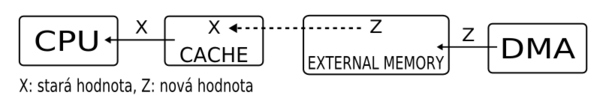
\includegraphics[width=12cm]{informatika/operacne_systemy_a_hw/obrazky/pametova_koherence.png}
  \caption{pam�ov� koherence}
\end{figure}

C�le I/O software:
\begin{pitemize}
    \item \textbf{Nez�vislost za��zen�}~-- programy nemus� dop�edu v�d�t, s jak�m p�esn� za��zen�m budou pracovat~-- je jedno jestli pracuji se souborem na pevn�m disku, disket� nebo na CD-ROM
    \item \textbf{Jednotn� pojmenov�n�} (na UNIXu /dev)
    \item \textbf{P�ipojen� (mount)}~-- �ast� u vym�niteln�ch za��zen� (disketa); mo�n� i u pevn�ch za��zen� (disk); nutn� pro spr�vnou funkci cache OS
    \item \textbf{Obsluha chyb}~-- v mnoha p��padech oprava bez v�dom� u�ivatele (velmi �asto zp�sobeno pr�v� u�ivatelem)
\end{pitemize}

\begin{reportN}{Bulej + Yaghob}
zapisal som vyse strany, ale to co ma yaghob na slidoch a to co je vo vypracovanom ucebnom texte ich ani trochu nezaujimalo. zaujimal ich popis DMA a preruseni, pricom sa pytali ako to presne funguje - chceli popisat instrukcie ako to moze prebiehat, ako sa to presne implementuje apod., co som bohuzial vobec nevedel
\end{reportN}

\begin{reportN}{Bulej} Prenos dat z disku do operacni pameti. P�ekvapiv� dobr� v�sledek, nicm�n� den p�edt�m jsem si �etl o DMA, tak�e bych to m�l v�d�t �ejo :-) Cht�l by prej je�t� v�d�t, �e to, co sed� na sb�rnici a ��d� ten p�enos, se ovl�d� z procesoru tak, �e v tom jsou n�jak� registry, do kterejch se hod� instrukce, a taky �e se na�tou data z disku do diskov� cache, pak se vyvol� p�eru�en�, a pak se teprva ty data n�jak dostanou do RAMky, t�ebas tim DMA nebo jinejma zp�sobama (a jakejma, pochopiteln�).
\end{reportN}

\subsection{Technologie d�lkov�ho p�enosu dat}

TODO: v�echno

\subsection{Velkokapacitní záznamová média, zálohování, technologie ukládání a zabezpečení záznamů}

TODO: všechno

\subsection{Architektury OS}

\begin{obecne}{Klasick� struktura~-- monolitick�}
Nejstar��, u� IBM 360, Unix, Windown 95-ME, v�echny slu�by uvnit�, prov�d�ny ve chr�n�n�m m�du, j�dro pom�rn� velk�, \uv{�dajn�} nejrychlej��. Program zavol� slu�bu OS, p�es tabulku se zjist� adresa p��sl. fce, ta se zavol� a vr�t� v�sledek.  Nev�hoda: hor�� �dr�ba -- je-li v programu chyba, m��e po�kodit zb�vaj�c� ��sti syst�mu, roz�i�ov�n� za b�hu je komplikovan�. 
\end{obecne}

\begin{obecne}{Virtu�ln� stroje}
P�vodn� n�pad : Virtual Machine pro IBM360 -- odd�lit multitasking od OS jako ext. stroj. Nad HW byla dal�� vrstva -- \uv{Virtual Machine} -- m�la pl�novat, vyr�b� pro procesy iluzi hol�ho HW; dneska nap�. VMWare d�l� to sam�. Pro IBM360 se dalo pou��t v kombinaci s CMS (jedno�lohov�) i p�vodn�ho OS360 (rychlej�� ne� OS360 na hol�m HW). 

Dnes: definuji abstraktn� stroj, pro n�j p�ekl�d�m programy (.NET, Java) $\rightarrow$ p�enositelnost, kompatibilita (IBM AS400~-- des�tky let), probl�m~-- pomal�. 
\end{obecne}

\begin{obecne}{Mikroj�dro}
snaha aby ��st b��c� v kernel m�du byla co nejmen�� (t�eba jen cca 10 KB), nejnov�j��, experiment�ln�, �asto pro Distribuovan� OS (dnes u� nepou��van�), hodn� proces� \& komunikace (klient/server), mikroj�dro �e�� jenom komunikaci. 

Filesyst�m apod. jsou procesy -- aplikace jim pos�laj� p�es j�dro po�adavky.

v�hoda: kdy� n�co spadne, nepo�kod� to zbytek, moduly jdou m�nit za b�hu, komunikace jde snadno roz���it na komunikaci po s�ti. Pou��vaj� ho: Chorus (�st�edny), QNX a Symbian OS.
\end{obecne}

  \begin{center}
    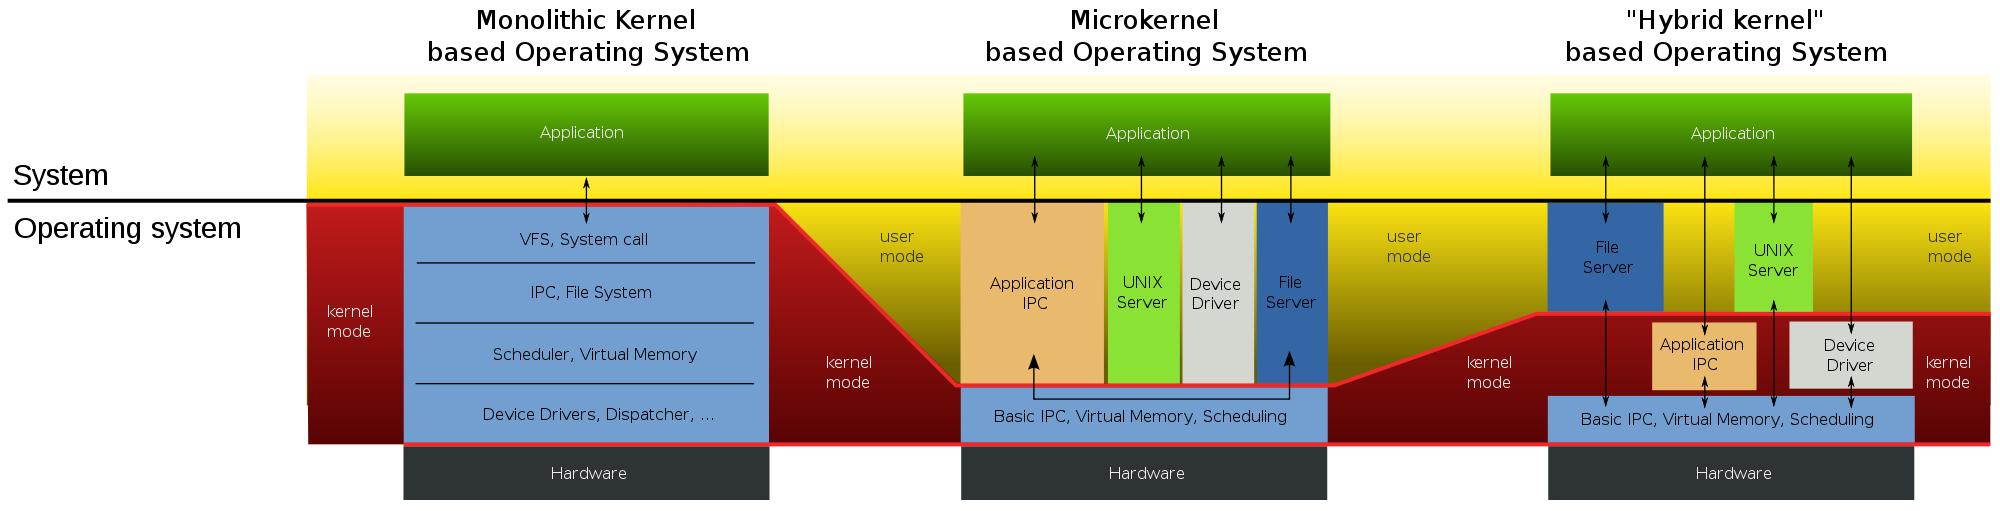
\includegraphics[width=19cm]{informatika/operacne_systemy_a_hw/obrazky/kernel.png}
  \end{center}

\begin{obecne}{Architektura WinNT}
  J�dro je pom�rn� mal� (cca 1MB), schopn� (pro vy��� vrstvy jsou n�kter� schopnosti skryt� - \textit{hybridn� j�dro}), na jeho vzniku se pod�leli schopn� Unix��i. Byla zde snaha o malou velikost, p�enositelnost. J�dro je neutr�ln� vzhledem k vy���m vrstv�m, nad n�m lze vybudovat r�zn� syst�my (Windows subsyst�m, POSIX, OS/2).

  Rozhran� OS a u�iv. program� zaji��uje WinAPI, nad n�m se nach�zej� r�zn� DLL, mezi kernelem a HW je \uv{hardware abstraction layer}, tj. kernel lze jednodu�e upravit pro jin� architektury (Alpha, IA-64).
  Grafick� drivery jedin� maj� p��m� p��stup k HW (kv�li v�konu), ��sti API (USER, GDI) jsou implementovan� v j�d�e, p�echod mezi user a kernel re�imem zaji��uje ntdll.dll (a je tedy vyu��v�n v�emi programy). Ve�ker� slu�by a aplikace b�� v user m�du nad j�drem.

  \begin{center}
    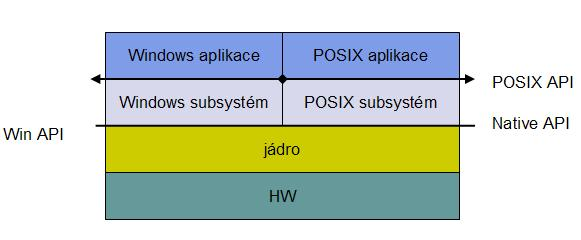
\includegraphics[width=8cm]{informatika/operacne_systemy_a_hw/obrazky/arch-windows.jpg}
  \end{center}
\end{obecne}

\begin{obecne}{Architektura Linuxu}
  \begin{pitemize}
      \item Na �rovni SW -- p�enositelnost; abstrakce HW. 
      \item nad HW~-- kernel, nad n�m syst�mov� vol�n�, hodn� podobn� Windows.
  \end{pitemize}

  \begin{center}
    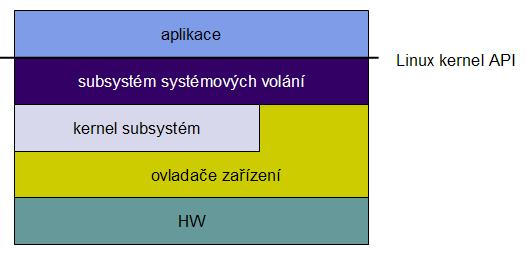
\includegraphics[width=8cm]{informatika/operacne_systemy_a_hw/obrazky/arch-linux.jpg}
  \end{center}
\end{obecne}


\subsection{Vztah OS a HW, obsluha přerušení}

\begin{obecne}{Zjištění změny stavu I/O zařízení:}
\begin{pitemize}
	\item \emph{asynchronní přerušení}~-- zašle zařízení
	\item \emph{polling}~-- peridická kontrola stavu zařízení
\end{pitemize}
\end{obecne}

\begin{obecne}{Druhy přerušení:}
\begin{pitemize}
	\item \emph{synchronní}~-- záměrně (instrukce TRAP~-- vstup do OS), výjimky (nesprávné chování procesu)~-- zpracuje se okamžitě
	\item \emph{asynchronní}~-- vnější událost (např. příchod dat)~-- zpracuje se po dokončení aktuální instrukce 
\end{pitemize}
\end{obecne}

\begin{obecne}{Obsluha přerušení:}
\begin{pitemize}
	\item OS se ujme řízení
	\item uloží se stav CPU (obsah registrů, čítač, ...)
	\item analyzuje se přerušení, vyvolá se příslušná obsluha (pokud není přerušení blokováno)
	\item obslouží se přerušení (např. se zavolá obslužná procedura)
	\item obnoví se stav CPU a aplikace pokračuje, popř. může dojít k přeplánování 
\end{pitemize}
\end{obecne}

\begin{obecne}{I/O software (vrstvy):}
\begin{pitemize}
	\item uživatelský I/O software
	\item I/O nezávislý subsystém
	\item ovladače zařízení
	\item obsluha přerušení 
\end{pitemize}
\end{obecne}

\begin{obecne}{Cíle I/O software:}
\begin{pitemize}
	\item nezávislost zařízení~-- programy nemusí vědět, s jakým přesně pracují
	\item jednotné pojmenování (/dev)
	\item připojení (mount)~-- vyměnitelná zařízení
	\item obsluha chyb
\end{pitemize}
\end{obecne}

\subsection{Procesy, vl�kna, pl�nov�n�}

\subsubsection*{Procesy a vl�kna}
Syst�mov� vol�n� je interface mezi OS (kernelspace) a u��vatelsk�mi programy (userspace).

\begin{e}{Definice}{0}{Proces}
  \emph{Proces} je in�tancia vykon�van�ho programu. Proces m� vlastn�
\textbf{pid (Process ID), pr�va (u�ivatele), adresn� prostor (pam�), vl�kna a otev�en� soubory}.
\end{e}

\obrazekvpravo{informatika/operacne_systemy_a_hw/obrazky/procesy_stavy.png}{P�echody mezi stavy procesu}{}{0.45}
\begin{e}{Stavy procesu}{0}{0}
Po�as �ivota sa m��e proces/vl�kno nach�dza� v r�znych stavoch:
\begin{pitemize}
  \item \emph{be��c�}~-- jeden proces/vl�kno na procesor,
  \item \emph{zablokovan�}~-- pri pou�it� blokuj�ceho volania~-- I/O disku at�.,
  \item \emph{p�ipraven�}~-- skon�ilo blokovanie; spotreboval v�etok pridelen� �as resp. vr�til riadenie syst�mu, �ak� na nov� pridelenie procesora,
  \item \emph{zombie}~-- po ukon�en� procesu, ke� u� nepracuje~-- ale e�te nebol vymazan�\footnote{taky stav zombie tam neni jenom kvuli vtipnosti; kdyz proces skonci
svoji cinnost, tak se treba muze cekat na to, az si navratovou hodnotu
procesu nekdo vyzvedne - a potom se proces muze oznacovat ve stavu
zombie }.
\end{pitemize}
\end{e}

\begin{e}{Organizace pam�ti procesu}{0}{0}

Pam� procesu (spu�t�n�ho programu) lze rozd�lit do n�kolika ��st�:
\begin{pitemize}
\item \emph{k�d programu (text segment)} \\
vytvo�en p�i p�ekladu, sou��st spustiteln�ho souboru, nem�nn� a m� pevnou d�lku; obvykle b�v� chr�n�n proti z�pisu
\item \emph{statick� data (data segment)} -- data programu, jejich� velikost je zn�ma ji� p�i p�ekladu a jejich� pozice se b�hem programu nem�n� (je p�ipraven kompil�torem a jeho form�t je takt� zadr�tovan� ve spustiteln�m souboru, u inicializovan�ch statick�ch dat je tam cel� ulo�en�); v jazyce C jde o glob�ln� prom�nn� a lok�ln� data deklarovan� jako \texttt{static} (prom�nn� alokovan� pouze jednou), konstanty
\item \emph{halda (heap segment)} -- vytv��en startovac�m modulem (C Runtime library), ukl�daj� se sem dynamicky vznikaj�c� objekty (\texttt{malloc, new})  neinicializovan� data, i seznam voln�ho m�sta. \\Halda zjemnuje to, co ti dovoluje spravce virtualni pameti. Ten ti dovoluje taky alokovat pamet a jinak s ni pracovat, ale protoze umi pracovat jen s celymi strankami (treba 4 KB velke), tak proste nekolikabajtove bloky od nej dostat primo nemuzes. A halda prave ty cele alokovane stranky rozdeluje do mensich bloku (postupne z nich ukrajuje, jak volas \texttt{malloc()})... pokud ji volna pamet dojde, alokuje si dalsi stranky... a tak dale.
\item \emph{voln� pam�} \\
postupn� j� zapl�uje z jedn� strany z�sobn�k a z druh� halda
\item \emph{z�sobn�k (stack segment)} \\
informace o vol�n� procedur (\uv{aktiva�n� z�znamy}) --- n�vratov� adresy, parametry a n�vratov� hodnoty (nejsou-li p�ed�v�ny v registrech), n�kter� jazyky (Pascal, C) pou��vaj� i pro �schovu lok�ln�ch prom�nn�ch. Typicky roste z�sobn�k proti hald� (od \uv{konce} pam�ti k ni���m adres�m).
\end{pitemize}
\end{e}

\begin{e}{Definice}{0}{Vl�kno (Thread)}
  \emph{Vl�kno} je mo�nos� pre program ako sa \uv{rozdeli�} na dva alebo viac
  z�rove� (resp. pseudo-z�rove�) vykon�van�ch �loh. Oproti procesu mu nie je
  pridelen� vlastn� pam�~-- je to len miesto vykon�vania in�trukci� v programe.
  Oproti procesu s� jeho \uv{atrib�tmi} len: \textbf{stav(+priorita), z�sobn�k, registrov CPU (i hodnotou PC\footnote{kdy� se vl�kno p�eru�� tak se ulo��
i to kam v n�m PC ukazoval - aby pak mohlo pokra�ovat kde zkon�ilo})}.
\end{e}
\begin{figure}[h]
  \centering
  \subfloat[Process control block]{\label{fig:pcb_process} 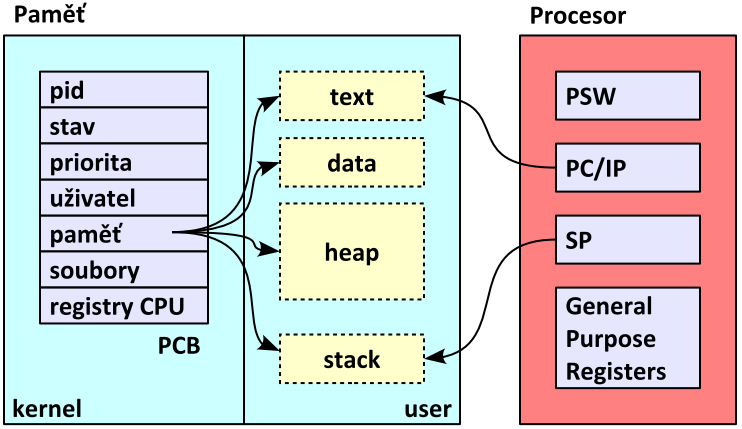
\includegraphics[width=8cm]{informatika/operacne_systemy_a_hw/obrazky/pcb_process_control_block.png}} \hfill
  \subfloat[Process control block s vl�kny]{\label{fig:pcb_thread}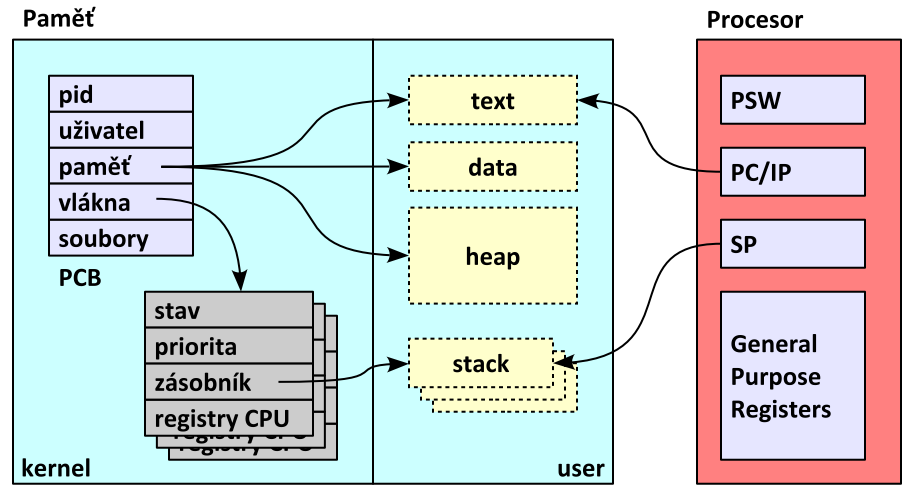
\includegraphics[width=8.5cm]{informatika/operacne_systemy_a_hw/obrazky/pcb_process_control_block_vlakna.png}}
  \caption{Process Control Block - execution context \footnotesize(v�imn�te si
  odd�len�ho kernel a user m�du)}
  \label{fig:pcb}
\end{figure}

\newpage
\textbf{Implementace:}
\begin{pitemize}
        \item \textbf{User Level Threads}(1.diagram) - thread management d�l� aplikace (nemus� b�t podporov�ny OS), ka�d� proces ma thread table, kdy� syst�m zablokuje proces zablokuj� se i v�echny jeho thready
        \item \textbf{Kernel Threads}(2.diagram) - thread management d�l� OS (mus� podporovat), thread table je glob�ln�, syst�m blokuje pouze jednotliv� thready
  \begin{center}
  \begin{center}
    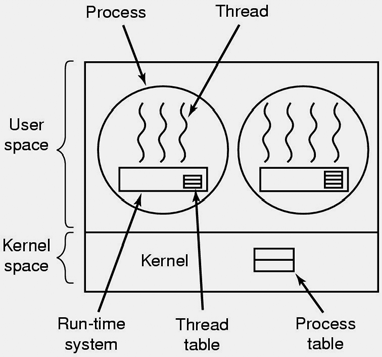
\includegraphics[height=6cm]{informatika/operacne_systemy_a_hw/obrazky/user-threads.png}
    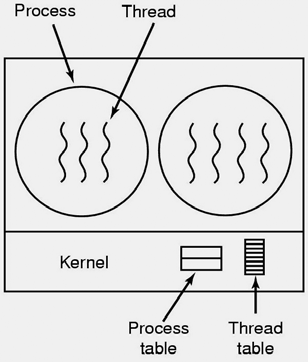
\includegraphics[height=6cm]{informatika/operacne_systemy_a_hw/obrazky/kernel-threads.png}
  \end{center}  
  \end{center}
\end{pitemize}
\emph{Multithreading} - schopnost syst�mu efektivn� pou��vat v�ce thread�, modely:
\begin{pitemize}
        \item \textbf{many-to-one (User Level Threads)} - mnoho user-level thread� je namapov�no na jednu kernel entitu, pou��v� se na syst�mech nepodporuj�c�ch kernel thready (nap�. Linux - GNU Portable Threads)
        \item \textbf{one-to-one (Kernel Threads)} - ka�d� user-level thread je namapov�n na jeden kernel thread (nap�. win2000, Linux - NGPT)
\end{pitemize}

\subsubsection*{Pl�nov�n�}

P�i pl�nov�n� procesoru se v opera�n�m syst�mu \textit{pl�nova�} (anglicky scheduler) rozhoduje, kter�mu procesu bude p�id�len procesor, a tedy kter� proces v n�sleduj�c�m �asov�m �seku bude procesor po��ta�e vyu��vat pro sv�j b�h. K pl�nov�n� procesoru doch�z� v n�sleduj�c�ch situac�ch:
\begin{pitemize}
        \item pokud n�kter� b��c� proces p�ejde do stavu blokovan�
        \item pokud n�kter� proces skon��
        \item pokud je b��c� proces p�eveden do stavu p�ipraven�
        \item pokud je n�kter� proces p�eveden ze stavu blokovan� do stavu p�ipraven�
\end{pitemize}
 Pl�novanie pritom m��e by� \textit{preempt�vn�} (v�t�inou pomoc� p�eru�en�, bez spolupr�ce s programem, pln� v re�ii OS - Windows NT, Linux) alebo \textit{nepreemptivn�} (vy�aduje spolupr�ci s programem, kooperat�vne~-- Windows 3.x).
\\\\
\begin{obecne}{Metriky OS pro pl�nov�n� proces�:}
\begin{pitemize}
 \item doba odezvy (response time, turnaround) -- do ukon�eni procesu, do prvni odezvy
 \item propustnost (throughput) -- po�et dokon�enych uloh za jednotku �asu
 \item vyu�iti procesoru (utilization)
 \item spravedlnost (fairness)
\end{pitemize}
\end{obecne}

\begin{obecne}{Algoritmy:}
\begin{pitemize}
        \item \textbf{First Come First Served (FCFS)}: nepreempt�vny, procesy pl�nov�ny v po�ad�, v jak�m p�ich�zej�, procesy b�� dokud neskon��
  \begin{center}
    \includegraphics[width=8cm]{informatika/operacne_systemy_a_hw/obrazky/fcfs.png}
  \end{center}
        \item \textbf{Round Robin}: preempt�vne roz��renie FCFS, ka�d� proces m� stejn� povolen� �asov� kvantum na b�h, po jeho uplynut� je proces p�esunut na konec fronty
  \begin{center}
    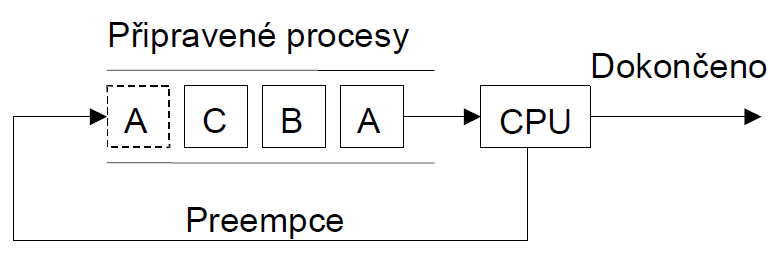
\includegraphics[width=8cm]{informatika/operacne_systemy_a_hw/obrazky/round-robin.png}
  \end{center}
        \item \textbf{Pl�novan� s n�kolika frontami}: ka�d� front� je p�i�azena
n�jak� priorita, bereme procesy s fronty s nejvy��� prioritou. Pokud vy�erp�
svoje �asov� quantum tak j� za�ad�me do fronty o �rove� n�.
  \begin{center}
    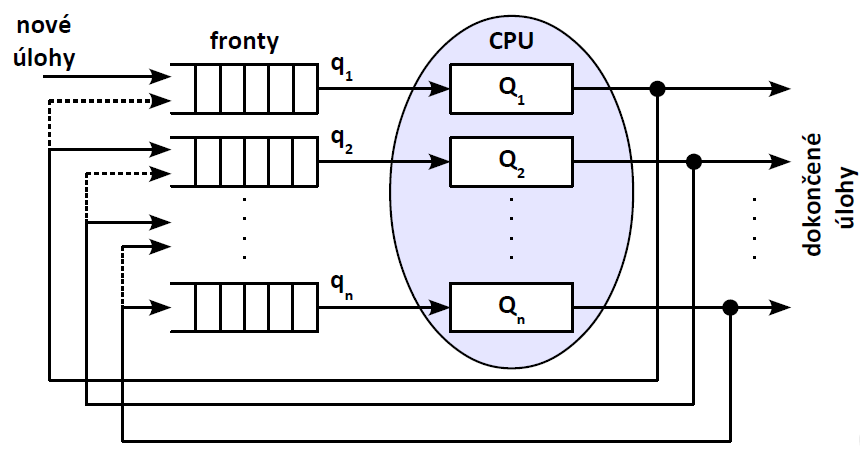
\includegraphics[width=8cm]{informatika/operacne_systemy_a_hw/obrazky/vice-front.png}
  \end{center}

        \item \textbf{Symmetric multiprocessing (SMP)}: druh v�ceprocesorov�ch syst�m�, u kter�ch jsou v�echny procesory v po��ta�i rovnocenn�,  fronta CPU �akaj�cich na pripraven� procesy (akt�vne (spotrebov�va energiu) vs. pas�vne �akanie (�peci�lne in�trukcie)), \uv{vz�ah}/afinita procesov k CPU
        \end{pitemize}
\end{obecne}

\begin{reportN}{Zavoral}
zhruba to co je vo vypiskach, diskusia dalej pokracovala o rozdieloch medzi vlaknami a procesmi - napr ako su implementovane vlakna v OS ktory ich nepodporuje (snazil som sa to nejak ukazat na JVM, ale podrobnosti som velmi nevedel, takze to bolo dost napovedy pana Zavorala a par slov odo mna :? ).
\\\\
n�kdo jiny: som letel na Vlaknach (nevedel som ze su reprezentovane hodnotou registrov, prog. citaca a zasobnikom)
\end{reportN}

\subsection{Synchroniza�n� primitiva, vz�jemn� vylou�en�}

\subsubsection*{Pojmy}

\begin{description}
  \item[�asov� z�visl� chyby (Race Conditions)] Situace kde 2 nebo v�ce proces� p�istupuje ke stejn�mu sd�len�mu prost�edku, a fin�ln� v�sledek z�le�� na kdo prob�hne kdy se jmenuje \emph{race conditions}

  P��klad na tiskov� front�:
  \begin{center}
    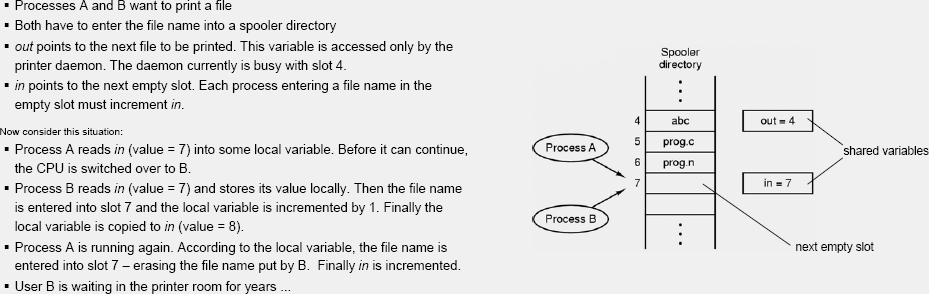
\includegraphics[width=13cm]{informatika/operacne_systemy_a_hw/obrazky/race-conditions.png}
  \end{center}

        \item[Kritick� sekce (Critical Regions)] ��st programu, kter� dokud nen� dokon�ena nen� mo�n� za��t jinou (nap�. pou��v� sd�len� prost�edky)
  \begin{center}
    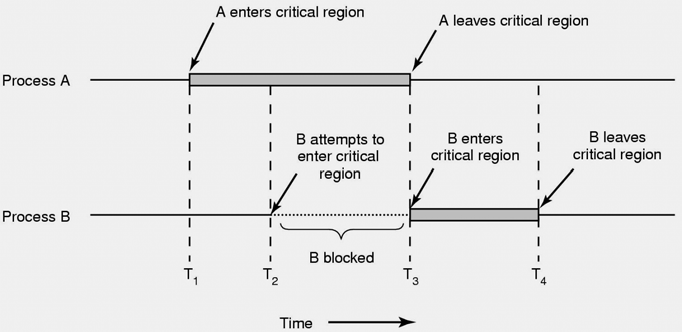
\includegraphics[width=9cm]{informatika/operacne_systemy_a_hw/obrazky/critical-region.png}
  \end{center}  
  
        \item[Vz�jemn� vylou�en� (Mutual Exclusion)] kritickou operaci prov�d� nejv��e jeden proces. Podm�nky vz�jemn�ho vylou�en�:
\begin{penumerate}
        \item ��dn� dva procesy nemohou b�t najednou ve stejn� kritick� sekci
        \item Nemohou b�t u�in�ny ��dn� p�edpoklady o rychlosti procesu (��dn� odhady rychlosti nebo priorit procesu, mus� fungovat se v�emi procesy)
        \item ��dn� proces mimo kritickou sekci nesm� blokovat jin� proces
        \item ��dn� proces nesm� �ekat nekone�n� dlouho v kritick� sekci (jinak dead-lock)
\end{penumerate}
Metody dos�hnut� vz�jemn�ho vylou�en�: aktivn� �ek�n� (busy waiting) a pasivn� �ek�n�/blokov�n�.
\end{description}

\subsubsection*{Aktivn� �ek�n� (Busy Waiting)}
\emph{Vlastnosti}: \textbf{spot�ebov�v� �as procesoru}, vhodn�j�� pro p�edpokl�dan� kr�tk� doby �ek�n�, nespot�ebov�v� prost�edky OS, rychlej��.

Navrhovan� �e�en�: 
\begin{pitemize}
  \item \textbf{Zak�z�n� p�eru�en�}] nevhodn� - proces m� plnou kontrolu nad po��ta�em 
  \item \textbf{Z�mky v prom�nn�}] nefunguj� - mezi p�e�t�n�ma nastaven�m locku m��e b�t program p�eru�en - pak by si "nev�im" lock == 1 a vesel pokra�oval, akor�t jsme p�idali novou race condition. 
\begin{verbatim}
int lock;
void proc(void) {
  for (;;) {
    nekritick�_sekce();
    while (lock != 0);
    lock = 1;
    kritick�_sekce();
    lock = 0;
  }
}
\end{verbatim}
  \item \textbf{D�sledn� st��d�n� (Strict Alternation)} funguje ale poru�uje podm�nku 3 - prom�nn� turn hl�d� kdo je na �ad�

\begin{verbatim}
int turn = 0;

void p1(void)                void p2(void)
{                            {
  for (;;) {                   for (;;) {
    while (turn != 0);           while (turn != 1);
    kritick�_sekce();            kritick�_sekce();
    turn = 1;                    turn = 0;
    nekritick�_sekce();          nekritick�_sekce();
  }                            }
}                            }
\end{verbatim}

  \begin{center}
    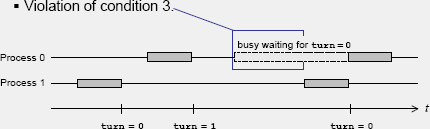
\includegraphics[width=9cm]{informatika/operacne_systemy_a_hw/obrazky/strict-alternation.png}
  \end{center}

\emph{Petersonovo �e�en�} - zobecn�n� pro N proces�:
\begin{verbatim}
#define N 2                   /* po�et proces� */
�
int turn;
int interested[N];            /* kdo m� z�jem */
�
void enter_region(int proc) { /* proc: kdo vstupuje */
int other = 1-proc;             /* ��slo opa�n�ho procesu */
    interested[proc] = TRUE;    /* m�m z�jem o vstup */
    turn = proc;                /* nastav p��znak */
    while (turn == proc && interested[other] == TRUE);
}
�
void leave_region(int proc) { /* proc: kdo vystupuje */
    interested[proc] = FALSE;   /* u� odch�z�m */
}
\end{verbatim}
 
  \item \textbf{Instrukce Test-and-Set Lock (TSL)} - atomick� operace na �rovni strojov�ho k�du, nem��e b�t p�eru�ena je nutn� aby ji podporoval HW (v�echny sou�asn� procesory n�jakou maj�):
\\
- implementace spin-locku (druh z�mku, na n�j� je t�eba aktivn� �ekat � �ekaj�c� proces p�i �ek�n� na spinlock spot�ebov�v� syst�mov� prost�edky) - po��d ale m�n� prost�edk� ne� p�edchoz� �e�en�  
\begin{verbatim}
enter_region:
    tsl   R,lock           ; na�ti z�mek do registru R a    
                           ; nastav z�mek na 1                        
    cmp   R,#0             ; byl z�mek nulov�?
    jnz   enter_region     ; byl-li nenulov�, znova
    ret                    ; n�vrat k volaj�c�mu - vstup do
                           ; kritick� sekce
�leave_region:
    mov   lock,#0          ; ulo� do z�mku 0
    ret                    ; n�vrat k volaj�c�mu
\end{verbatim}
\end{pitemize}

\subsubsection*{Pasivn� �ek�n�}
\emph{Vlastnosti}: proces je ve stavu blokov�n, vhodn� pro del�� doby �ek�n�, \textbf{spot�ebov�v� prost�edky OS}, pomalej��.

Postup pou��vaj�c� Sleep/Wakeup (implementov�ny OS, atomick� operace - sleep usp� volaj�c� proces, wakeup probud� udan� proces) nefunguje (viz Probl�m producent/konzument).
\begin{pitemize}
\item \textbf{Semafory} -- po��t� po�et probuzen�ch, reprezentace voln�ch a p�id�len�ch prost�edk�

Atomick� operace (nesm� b�t p�eru�eny):

\begin{description}
\item[down(semaphore* s)] -- zabere semafor (\verb=s--;=) pokud je voln� (\verb=s>0=), jinak �ek� na uvoln�n�

\item[up(semaphore* s)] -- uvoln� semafor (\verb=s++;=), vzbud� �ekaj�c� proces (pokud existuje)
\end{description}
-nutn� podpora OS (v�t�inou v kernelu)
 

\item \textbf{Mutex}
�peci�lny (bin�rny) typ semaforu, kde s� povolen� len hodnoty 0 a 1 (v Up sa miesto $s:=s+1$ vol� $s:=1$) sa naz�va \emph{mutex} a pou��va sa na riadenie pr�stupu k jednej premennej. V�t�inou pomoc� TSL.

\item \textbf{Monitory}
\par Implementov�ny p�eklada�em, lze si p�edstavit jako t��du C++ (v�echny prom�nn� priv�tn�, funkce mohou b�t i ve�ejn�), vz�jemn� vylou�en� v jedn� instanci (zaji�t�no synchronizac� na vstupu a v�stupu do/z ve�ejn�ch funkc�, synchronizace implementov�na blokovac�m primitivem OS). ???TODO

\item \textbf{Zpr�vy}
\par Operace SEND a RECEIVE, zablokov�n� odes�latele/p��jemce, adresace proces/mailbox, rendez-vous...

\item \textbf{RWL - read-write lock}, \textbf{bari�ry}...

Ekvivalence primitiv - pomoc� jednoho blokovac�ho primitiva lze implementovat jin� blokovac� primitivum.

Rozd�ly mezi platformami: Windows - jednotn� funkce pro pasivn� �ek�n�, �ek�n� na v�ce primitiv, timeouty. Unix - OS implementuje semafor, knihovna pthread.
\end{pitemize}
\subsubsection*{Klasick� synchroniza�n� probl�my}
\begin{pitemize}
\item \textbf{Probl�m producent/konzument}
\par Producent vyr�ba predmety, konzument ich spotreb�va. Medzi nimi je buffer pevnej ve�kosti (N). Konzument nem� �o spotreb�va� ak je buffer pr�zdny; producent prestane vyr�ba�, ak je buffer pln�. 

\begin{verbatim}
int N = 100;
int count = 0;
void producer(void) {
    int item;
    while(TRUE) {
        produce_item(&item);
        if(count==N) sleep ();
        enter_item(item);
        count++;
        if(count == 1) wake(consumer);
    }
}
void consumer(void) {
    int item;
    while(TRUE) {
        if(count==0) /*pozice A*/ sleep ();
        remove_item(&item);
        count--;
        if(count==N-1)
            wake(producer);
        consume_item(&item);
    }
}
\end{verbatim}

\begin{penumerate}
        \item Buffer je pr�zdny, a konzument pr�ve pre��tal count, aby zistil, �i je rovn� nule
        \item Prepl�novanie na producenta ("pozice A")
        \item Producent vytvo�� item a zv��� count
        \item Producent zist�, �i je count rovn� jednej. Zist� �e �no, �o znamen� �e konzument bol predt�m zablokovan� (preto�e muselo by� 0), a zavol� wakeup
        \item Teraz m��e d�js� k zablokovaniu: konzument pokra�uje na "pozici
A" a usp� se, preto�e si mysl�, �e nem� �o zobra�; producent bude chv��u produkova� a d�jde "preplneniu" $\Rightarrow$ usp� sa; sp� producent aj konzument :o) 
\\\\
�e�en� pomoc� semaforu:\\
\begin{verbatim}
#define N 10
typedef int semaphore;     //a semaphore is an integer
semaphore empty = N;       //counting empty slots
semaphore full = 0;        //counting full slots
semaphore mutex = 1;       //mutual exclusion on buffer access

void producer() {
  while (TRUE) {
    int item = produce_item();
    down(&empty);          //possibly sleep, decrement empty counter
    down(&mutex);          //possibly sleep, claim mutex (set it to 0) thereafter
    insert_item(item);
    up(&mutex);            //release mutex, wake up other process
    up(&full);             //increment full counter, possibly wake up other ...
  }
}

void consumer() {
  while(TRUE) {
    down(&full);           //possibly sleep, decrement full counter
    down(&mutex);          //possibly sleep, claim mutex (set it to 0) thereafter
    item = remove_item();
    up(&mutex);            //release mutex, wake up other process
    up(&empty);            //increment empty counter, possibly wake up other ...
    consume_item(item);
  }
}
\end{verbatim}

\end{penumerate}
\item \textbf{Probl�m ob�dvaj�c�ch filosof�}
\par P�t filosof� sed� okolo kulat�ho stolu. Ka�d� filosof m� p�ed sebou tal�� �paget a jednu vidli�ku. �pagety jsou bohu�el slizk� a je t�eba je j�st dv�ma vidli�kami. �ivot filosofa sest�v� z obdob� j�dla a obdob� p�em��len�. Kdy� dostane hlad, pokus� se vz�t dv� vidli�ky, kdy� se mu to poda��, naj� se a vidli�ky odlo��.

\item \textbf{Probl�m ospal�ho holi�e}
\par Holi� m� ve sv� ofic�n� k�eslo na holen� z�kazn�ka a pevn� po�et seda�ek pro �ekaj�c� z�kazn�ky. Pokud v ofic�n� nikdo nen�, holi� se posad� a sp�. Pokud p�ijde prvn� z�kazn�k a holi� sp�, probud� se a posad� si z�kazn�ka do k�esla. Pokud p�ijde z�kazn�k a holi� u� st�ih� a je voln� m�sto v �ek�rn�, posad� se, jinak odejde.
\end{pitemize}


\begin{reportN}{Bulej}
\begin{penumerate}
        \item priklad Producent-konzument pomoci semaforu

        \item stacilo napsat aktivni vs. pasivni, kriticka sekce, spinlock, semafor (obecne monitor) a pak nasledovalo par otazek, zda je mozne naprogramovat synch. primitivum bez podpory HW
\end{penumerate}
\end{reportN}

\begin{reportN}{Bulej}
Mysl�m, �e jsem je pochopil, a� kdy� mi to pan Skopal vysv�tlil. To, co je v materi�lech opravdu nesta��. TSL je dobr� v tom, �e m� prav� operaci Test and Set Lock jako atomickou. Pak jsem se pokou�el ud�lat semafor pro probl�m producent a konzument a d�lal jsem ho upln� �patn�
\end{reportN}

\begin{reportN}{Hn�t�nka}
na jedni�ku mus�te um�t praktick� u�it� (nap�. z v�ce mutex� postavit semafor)
\end{reportN}

\begin{reportN}{Bedn�rek}
Na tuhle jsem byl p�ipraven� ze zadan�ch ot�zek asi nejh��, kupodivu jsem toho k n� ale nakonec na pap�r vyplodil pom�rn� dost a dostal k t�matu jen m�lo dopl�uj�c�ch ot�zek (n�jak� drobn� praktick� a jak implementovat mutex bez podpory OS, tj. pomoc� test-and-set instrukce), pak se plynule a nepozorovan� p�e�lo na zablokov�n� a zotaven� z n�j. N�co jsem v�d�l, vzpomn�l jsem si na 3 ze 4 Coffmanov�ch podm�nkek a jejich o�et�en�, �tvrtou jsem pak vymyslel s Bedn�rkovou vydatnou pomoc�. ��dn� ot�zky na "klasick� synchroniza�n� probl�my" nebo Petersonovo �e�en�, tj. v�ci, o kter�ch jsem se s�m rad�i nezm�nil.

na konci sa opytal, ze aky problem okrem vyhladovania moze nastat... deadlock

Sleep/wakeup, semafory, monitory, spr�vy, polling - u ka�d�ho ako funguje a �i to rob� aplik�cia/OS/HW. Potom sme sa pobavili o mo�nosti implementova� jedno druh�m. 
\end{reportN}

\subsection{Zablokov�n� a zotaven� z n�j}

Prost�edek je cokoliv, k �emu je pot�eba hl�dat p��stup (HW za��zen�~-- tisk�rny, cpu; informace~-- z�znamy v DB). Je mo�n� je rozd�lit na \emph{odn�mateln�} (lze odejmout procesu bez n�sledk�~-- CPU, pam�) a \emph{neodn�mateln�} (nelze odejmnout bez nebezpe�� selh�n� v�po�tu~-- CD-ROM, tisk�rna... tento druh zp�sobuje probl�my).

Pr�ce s prost�edky prob�h� v n�kolika kroc�ch: \emph{��dost o prost�edek} (blokuj�c�, pr�v� tady doch�z� k zablokov�n�), \emph{pou��v�n�} (nap�. tisk), \emph{odevzd�n�} (dobrovoln�/p�i skon�en� procesu).

Mno�ina proces� je \emph{zablokov�na}, jestli�e ka�d� proces z t�to mno�iny �ek� na ud�lost, kterou m��e zp�sobit pouze jin� proces z t�to mno�iny.

\subsubsection*{Coffmanovy podm�nky}
Splnenie t�chto podmienok je nutn� pre zablokovanie:
\begin{penumerate}
	\item \textbf{V�lu�n� p��stup} � ka�d� prost�edek je bu� vlastn�n pr�v� jedn�m procesem nebo je voln�.
	\item \textbf{Dr� a �ekej} � procesy aktu�ln� vlastn�c� n�jak� prost�edky mohou ��dat o dal��.
	\item \textbf{Neodn�matelnost} � p�id�len� prost�edky nemohou b�t proces�m odebr�ny.
	\item \textbf{�ek�n� do kruhu} � existuje kruhov� �et�z proces�, kde ka�d� z nich �ek� na prost�edek vlastn�n� dal��m �l�nkem �et�zu.
\end{penumerate}

\subsubsection*{�e�en� zablokov�n�}
\begin{pitemize}
	\item \textbf{P�tros� algoritmus}~-- Zablokov�n� se ani nedetekuje, ani se mu nezabra�uje, ani se neodstra�uje, U�ivatel s�m rozhodne o �e�en� (kill). Nespot�ebov�v� prost�edky OS~-- nem� re�ii ani neomezuje podm�nky provozu. (Nej�ast�j�� �e�en�~-- Unix, Windows) 
  \item \textbf{Detekce a zotaven�}~-- Hled� kru�nici v orientovan�m grafu (hrany vedou od procesu, kter� �ek�, k procesu, kter� prost�edek vlastn�), pokud tam je kru�nice, nastalo zablokov�n� a je t�eba ho �e�it:
		\begin{pitemize}
			\item \emph{Odebr�n� prost�edku}~-- dohled oper�tora, pouze na p�echodnou dobu
			\item \emph{Zab�jen� proces� z cyklu} (resp. mimo cyklus vlastn�c� identick� prost�edek)
			\item \emph{Rollback} (OS ukl�d� stav proces�, p�i zablokov�n� se n�kter� procesy vr�t� do p�edchoz�ho stavu $\Rightarrow$ ztracena pr�ce... obdoba u DB)
		\end{pitemize}
	\item \textbf{Vyh�b�n� se}~-- Bezpe�n� stav (procesy/prost�edky nejsou zablokov�ny, existuje cesta, jak uspokojit v�echny po�adavky na prost�edky spou�t�n�m proces� v jist�m po�ad�); Vi�. bank���v algoritmus. Nutn� je p�edem zn�t v�echny prost�edky, kter� budou programy pot�ebovat; OS pak d�v� prost�edky tomu, kter� je nejbl� sv�mu maximu pot�eby a nav�c pro kter� je prost�edk� dost na dokon�en�. Dnes se moc nepou��v�.
	\item \textbf{P�edch�zen� (prevence)}~-- napaden� jedn� z Coffmanovy podm�nek
		\begin{penumerate}
			\item \emph{V�lu�n� p��stup}~-- \emph{spooling} (prostriedky spravuje jeden systemov� proces, ktory dohliada na to, aby jeho stav bol konzistentny (tiskarna)~-- pozor na m�sto na disku)
			\item \emph{Dr� a �ekej}~-- ��dat o v�echny prost�edky p�ed startem procesu. Nejprve v�echno uvolnit a pak znovu ��dat o v�echny najednou
			\item \emph{Neodn�matelnost}~-- odn�mateln� prost�edky mohou b�t odejmuty bez n�sledk� (procesor-p�epl�nov�n�, pam�-swapping), neodn�mateln� nelze bez nebezpe�� selh�n� v�po�tu
			\item \emph{�ek�n� do kruhu}~-- v�echny prost�edky jednozna�n� o��slov�ny (sta�� prost�edky v n�jak�m kontextu), procesy mohou ��dat o prost�edky jen ve vzestupn�m po�ad�

		\end{penumerate}
			\item \emph{Dvojf�zov� zamyk�n�}~-- nejprve postupn� v�echno zamyk�m (prvn� f�ze). Potom se m��e pracovat se zam�en�mi prost�edky~-- a na z�v�r se u� jen odemyk� (druh� f�ze)~-- vi� transak�n� spracov�n� u datab�z� ((striktn�/konzervativn�) dvouf�zov� zpracov�n�)
\end{pitemize}

\textbf{Bank���v algoritmus}: Bank�� m� klienty a t�m sl�bil jistou v��ku �v�ru. Bank�� v�, �e ne v�ichni klienti pot�ebuj� plnou v��i �v�ru najednou. Klienti ob�as nav�t�v� banku a ��daj� postupn� o prost�edky do maxim�ln� v��ky �v�ru. A� klient skon�� s obchodem, vr�t� bance vyp�j�en� pen�ze. Bank�� pen�ze p�j�� pouze tehdy, z�stane-li banka v bezpe�n�m stavu.
\\ Probl�my: slo�itost $O(N^2)$, po�adovan� info je typicky nedostupn�, efektivn�j�� b�v� �e�it a� vznikl� probl�my
\subsection{Organizace pam�ti, aloka�n� algoritmy}

\textbf{Hierarchie pam�ti} (sm�rem odshora dol� roste velikost, cena na bajt a rychlost kles�~-- a naopak\dots):
\begin{pitemize}
    \item \emph{registry CPU} --- 10ky-100vky bajt� (IA-32: obecn� registy p�r 10tek), IA-64~-- a� kB (extr�m), stejn� rychl� jako CPU. 
    \item \emph{cache} --- z pohledu aplikac� nen� p��mo adresovateln�; dnes ��dov� MB, rozd�len� podle ��elu, n�kolik vrstev. L1 cache (cca 10ky kB)~-- d�len� instrukce/data; L2 (cca MB) sd�len� instr\&data, b�� na rychlosti CPU (d��v b�vala pomalej��), servery~-- L3 (cca 10MB). Vyrovn�v� rozd�l rychlosti CPU a RAM. Vyu��v� lokality program� -- cyklen� na m�st�; sekven�n�ho p��stupu k dat�m. Pokud nenajdu co chci v cache -- \uv{cache-miss}, na��t� se pot�ebn� z RAM (po bloc�ch), jinak (v 95-7\% p��pad�) nastane \uv{cache-hit}, tj. po�adovan� data v cache opravdu jsou a do RAM nemus�m.
    \item \emph{hlavn� pam�} (RAM) --- p��mo adresovateln� procesorem, 100MB~-- GB; pomalej�� ne� CPU; CAS~-- doba p��stupu na ur�. m�sto~-- nejv�c zdr�uje (v 1 sloupci u� �te rychle, dat. tok dostate�n�), dal��~-- latence~-- doba ne� data dote�ou do CPU~-- hraje roli vzd�lenost (AMD- integrovan� �adi� v CPU) 
    \item \emph{pomocn� pam�} --- nen� p��mo adresovateln�, typicky HDD; n�h. p��stup, ale pomalej��. ~100GB, r�zn� druhy~-- IDE, SATA, SCSI; nejv�c zdr�uje p��stupov� doba (�as seeku) cca 2-10ms; obvykle sektor~-- 512 B; roli hraje i rychlost ot��en� (4200~-- 15000 RPM)~-- taky ��dov� ms. 
    \item \emph{z�lohovac� pam�} --- nejpomalej��, z teorie nejv�t��, dnes ale neplat�; typicky~-- p�sky; pro v�t�� kapacitu~-- autoloadery ; sekven�n� p��stup; dnes~-- kv�li rychlosti �asto z�lohov�n� RAIDem.
\end{pitemize}

\textbf{Spr�vce pam�ti}: ��st OS, kter� spravuje pam�ovou hierarchii se naz�v�\\spr�vce pam�ti (memory manager):
\begin{pitemize}
	\item udr�uje informace o voln�/pln� ��sti pam�ti
	\item star� se o p�id�lov�n� pam�ti
	\item a \uv{v�m�nu pam�ti s diskem}
\end{pitemize}

\textbf{P�i�azen� adresy}
\begin{pitemize}
	\item p�i p�ekladu (je ji� zn�mo um�st�n� procesu, generuje se absolutn� k�d, PS: statick� linkov�n�)
	\item p�i zav�d�n� (OS rozhodne o um�st�n�~-- generuje se k�d s relokacemi, PS: dynamick� linkov�n�)
	\item za b�hu (proces se m��e st�hovat i za b�hu, reloka�n� registr)
\end{pitemize}

\textbf{Overlay}~-- Proces pot�ebuje v�ce pam�ti ne� je skute�n� k dispozici.
Program�tor tedy rozd�l� program na nez�visl� ��sti (kter� s v pam�ti podle
pot�eby vym��nuj�) a ��st nezbytnou pro v�echny ��sti... Pou��v�no hlavn� v DOSu, nyn� se stejn�ho c�le dosahuje pomoc� virtu�ln� pam�ti

\textbf{V�m�na (swapping)}~-- d�l� se, proto�e proces mus� b�t v hlavn� pam�ti,
aby jeho instrukce mohly b�t vykon�v�ny procesorem... Jde o v�m�nu obsahu pam�ti
mezi hlavn� a z�lo�n�.

\textbf{P�eklad adresy}~-- nutn�, proto�e proces pracuje v logick�m (virtu�ln�m) adresov�m prostoru, ale HW pracuje s fyzick�m adresov�m prostorem...

\textbf{Spojit� p�id�lov�n� pam�ti}~-- p�id�len� jednoho bloku / v�ce pam�tov�ch odd�l� (\emph{pevn�}~-- pam� pevn� rozd�lena na ��sti pro r�zn� velikosti blok�/\emph{voln�}~-- v libovoln� ��sti voln� pam�ti m��e b�t alokov�n libovoln� velik� blok)

\textbf{Informace o obsazen� pam�ti}~-- bitov� mapa / spojov� seznam voln�ch blok� (spojov�n� uvoln�n�ho bloku se sousedy)

\textbf{Aloka�n� algoritmy}:
\begin{pitemize}
	\item \emph{First-fit}~-- prvn� voln� dostate�n� velikosti~-- rychl�, ob�as ale rozd�l� velkou d�ru
	\item \emph{Next-fit}~-- dal�� voln� dostate�n� velikosti, za��n� se na podledn� prohled�van� pozici~-- jako First-fit, ale rychlej��
	\item \emph{Best-fit}~-- nejmen�� voln� dostate�n� velikosti~-- pomal� (prohled�v� cel� seznam), zanech�v� malink� d�ry (ale nech�v� velk� d�ry vcelku)
	\item \emph{Worst-fit}~-- nejv�t�� voln�~-- pomal� (prohled�v� cel� seznam), rozd�l� velk� d�ry
	\item \emph{Buddy syst�m}~-- pam� rozd�lena na bloky o velikosti $2^n$, bloky stejn� velikosti v seznamu, p�i p�id�len� zaokrouhlit na nejbli��� $2^n$, pokud nen� voln�, roz�t�pnou se v�t�� bloky na p��slu�n� men�� velikosti, p�i uvoln�n� pam�ti se slu�uj� sousedn� bloky (buddy)
\end{pitemize}

\textbf{Fragmentace pam�ti}:
\begin{pitemize}
	\item \emph{extern�}~-- voln� prostor rozd�len na mal� kousky, pravidlo 50\% -- po n�jak� dob� b�hu programu bude cca 50\% pam�ti fragmentov�no a u toho to z�st�v� - pl�tv�n� m�stem mezi alokovan�mi oblastmi
	\item \emph{intern�}~-- nevyu�it� cel�ho p�id�len�ho prostoru (50\% velikosti posledn�ho bloku prostoru nevyu�ito) - pl�tv�n� m�stem uvnit� alokovan� oblasti
	\item \emph{sesyp�n�}~-- pouze p�i p�i�azen� adresy za b�hu, nebo segmentaci~-- nelze p�i statick�m p�id�len� adresy
\end{pitemize}

\subsection{Principy virtu�ln� pam�ti, str�nkov�n�, algoritmy pro v�m�nu str�nek, v�padek str�nky, str�nkovac� tabulky, segmentace}

\subsubsection*{Virtu�ln� pam�}

\obrazekvpravominipage{informatika/operacne_systemy_a_hw/obrazky/virtual-memory.png}{Virtu�l\-n�
pam�}{fig:virpamet}{0.15}{0.8}{

Virtu�ln� pam� zp�sob spr�vy opera�n� pam�ti po��ta�e, kter� umo��uje p�edlo�it b��c�mu procesu adresn� prostor pam�ti, kter� je uspo��d�n jinak nebo je dokonce v�t��, ne� je fyzicky p�ipojen� opera�n� pam� RAM. Z tohoto d�vodu procesor rozli�uje mezi virtu�ln�mi adresami (pracuj� s nimi strojov� instrukce, resp. b��c� proces) a fyzick�mi adresami pam�ti (odkazuj� na konkr�tn� adresov� bu�ky pam�ti RAM). P�evod mezi virtu�ln� a fyzickou adresou je zaji��ov�n samotn�m procesorem v MMU (je nutn� hardwarov� podpora) nebo samostatn�m obvodem. 
\\\\
�lo
by to bez HW podpory? Jist� �e ano VM to tak d�laj�, nicm�n� rychlost nen�
nijak os�uj�c�, proto se do novych stroj� u� p�id�v� jejich HW podpora (??
ov��it).
\begin{pitemize}
        \item Umo��uje sd�len� pam�ti (opera�n�m syst�mem)
        \item Vz�jemn� ochrana program� (v sou�asnosti je d�le�it�j�� ochrana dat ne� vyu�it�
principu lokalit), tzn. to aby jeden program nep�episoval druh�mu programu jeho
data a tak.
        \item Ka�d� b��c� program pracuje se \textbf{sv�m} virtu�ln�m adresn�m prostorem
\end{pitemize}
Existuj� dv� z�kladn� metody implementace virtu�ln� pam�ti � str�nkov�n� a segmentace.
}

\subsubsection*{Str�nkov�n�}
P�i str�nkov�n� je pam� rozd�lena na v�t�� �seky stejn� velikosti, kter� se naz�vaj� str�nky. Spr�va virtu�ln� pam�ti rozhoduje samostatn� o tom, kter� pam�ov� str�nka bude zavedena do vnit�n� pam�ti a kter� bude odlo�ena do odkl�dac�ho prostoru (swapu).
\\\\
Podporovan� v�emi velk�mi CPU a OS, jednorozm�rn� VAP (virtu�ln� adresn�
prostor).\begin{pitemize}
\item VAP rozd�len na str�nky (velikost je mocnina 2), FAP na r�mce (�seky stejn� d�lky)
\item \textbf{p�evod str�nkovac� tabulkou}  - ka�d� proces m� svoj�, p��znak existence mapov�n� (v.str�nka nen� v FAP \rightarrow$ ud�lost "v�padek str�nky" \rightarrow$ synchronn� p�eru�en�) um�st�na v fyzick� pam�ti
\par \begin{center}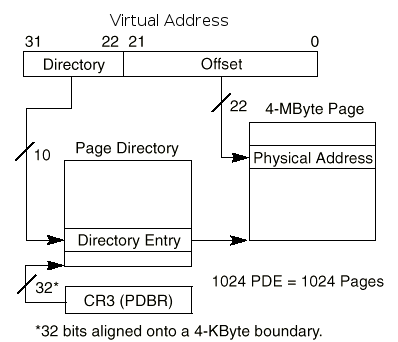
\includegraphics[width=5cm]{informatika/operacne_systemy_a_hw/obrazky/strankovani1_new.png}\end{center}
\item umo�nuje \emph{odd�len� VAP} i \emph{sd�lenou pam�} - mapov�n� virtu�ln� str�nky 2 proces� na jednu fyzickou
\item OS m�n� tabulky str�nek zm�nou PTBR (Page Table Base Register) - PTBR obsahuje
b�zovou adresu tabulky str�nek procesu
\item P��klad: polo�ka str�nkovac� tabulky Intel IA32 (= x86) $\rightarrow$ jej� struktura je z�visl� na architektu�e CPU
\par \begin{center} 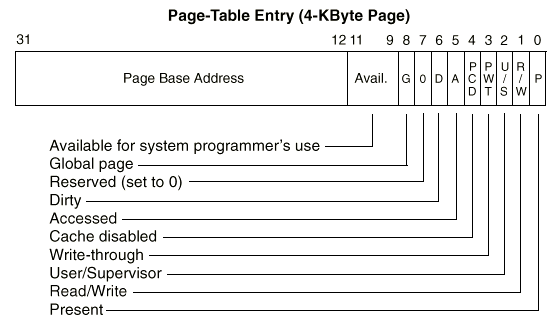
\includegraphics[width=6cm]{informatika/operacne_systemy_a_hw/obrazky/strankovani-polozka.png} \end{center}
\item \textbf{v�ce�rov�ov� str�nkov�n�} (nap�. kv�li velikosti - jedna tabulka
je u� moc velk� =\textgreater pomal�)
\par \begin{center} 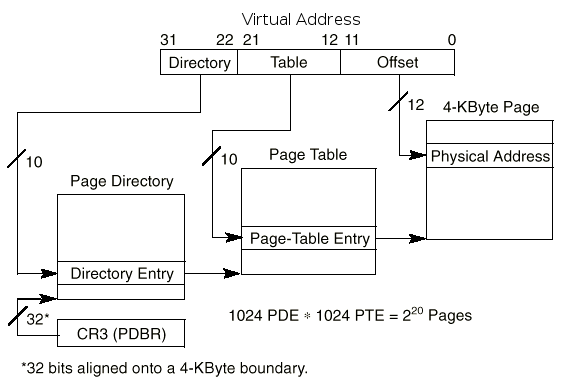
\includegraphics[width=6cm]{informatika/operacne_systemy_a_hw/obrazky/strankovani2_new.png} \end{center}
\item \textbf{TLB (Translation Lookaside Buffer)} - asociativn� pam� slou��c� na rychl�  mapov�n� virtu�ln� str�nky na fyzickou, vyhled�v� se v n� paraleln�, typicky ma 128-256 polo�ek, vyu��v� princip prostorov� lokality program� (v�t�ina program� prov�d� velk� po�et p��stup� k mal�mu
po�tu str�nek)
um�st�va v�t�inou v L1 nebo L2 cache na procesoru
\par 
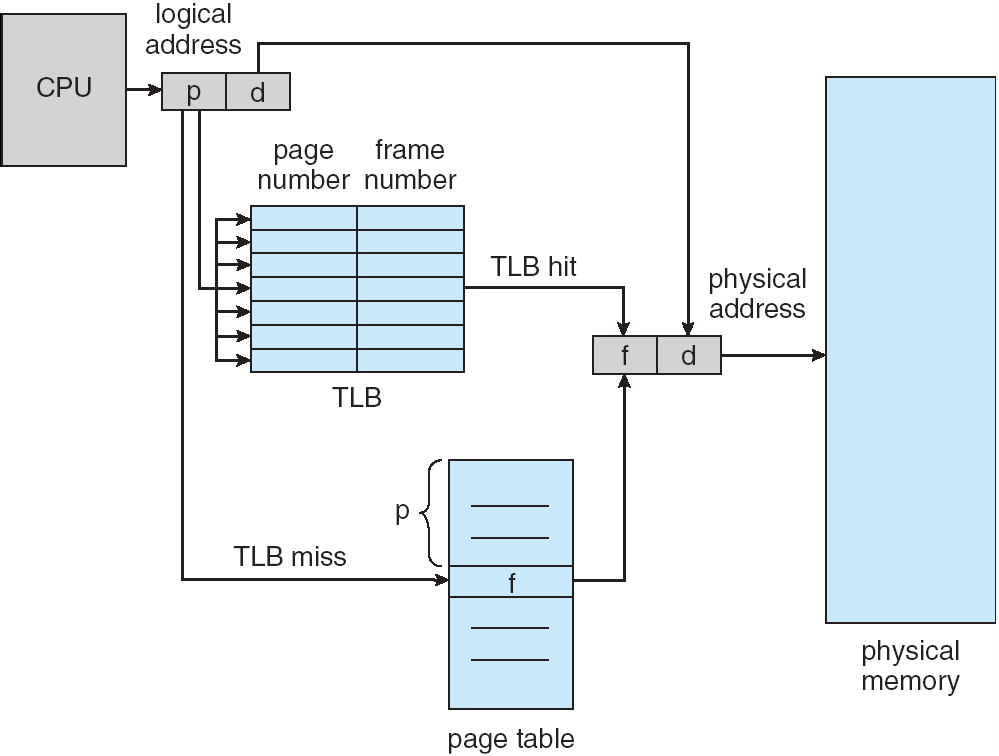
\includegraphics[width=6cm]{informatika/operacne_systemy_a_hw/obrazky/strankovani-tlb-schema.png}
\caption{~~~}
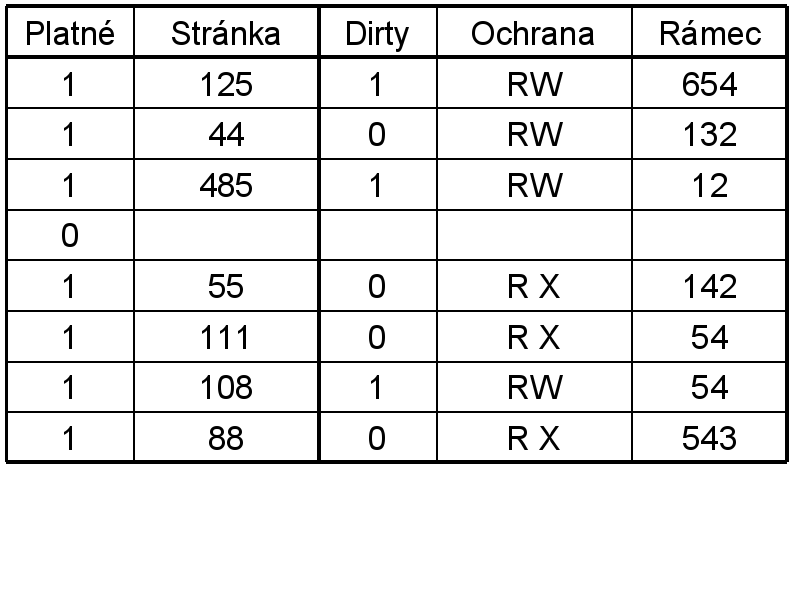
\includegraphics[width=5cm]{informatika/operacne_systemy_a_hw/obrazky/strankovani-tlb.png}
 
\par ...\textbf{0-�rov�ov� str�nkov�n�} - procesor hled� pouze TLB, zbytek
�e�� OS (obl�ben� u 64-bitov�ch CPU - UltraSPARC III)
\item \textbf{inverzn� str�nkov�n�} (nap�. kdy� FAP je men�� ne� VAP, 64-bitov� CPU - IA-64 = UtraSPARC, PowerPC)
- inverzn� str�nkovac� tabulka (IPT) nad r�mci (nikoliv str�nkami) spole�n�
pro v�echny procesy, pro vyhled�v�n� se pou��v� hashovac� tabulka\par \begin{center} 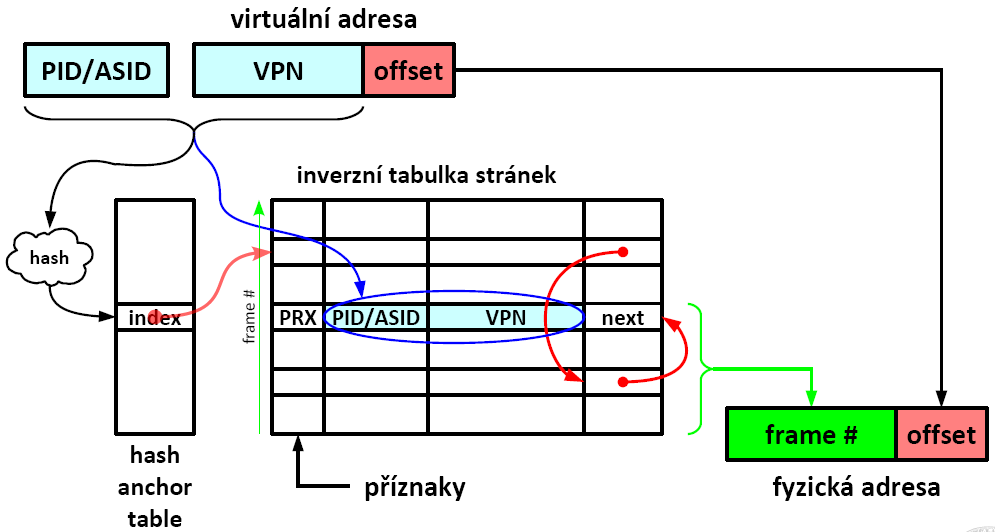
\includegraphics[width=10cm]{informatika/operacne_systemy_a_hw/obrazky/strankovani-inv_new.png} \end{center}
\end{pitemize}

\begin{obecne}{Akce vykon�van� p�i v�padku str�nky:}
\begin{pitemize}
\item v�jimka procesoru
\item ulo�it stav CPU (kontext)
\item zjistit VA
\item kontrola platnosti adresy a pr�v
\item nalezen� vhodn�ho r�mce
\item zru�it mapov�n� na nalezen� r�mec
\item pokud je vyhazovan� r�mec vyhazov�n, spustit ukl�d�n� na disk
\item na��st z disku po�adovanou str�nku do r�mce
\item zav�st mapov�n�
\item obnovit kontext
\end{pitemize}
\end{obecne}

\begin{obecne}{P�i implementaci str�nkov�n� je nutno brat v �vahu:}
\begin{pitemize}
    \item \emph{znovuspu�t�n� instrukce} --- je pot�eba aby procesor po v�padku zkusil p��stup do pam�ti znova. dnes um� v�echny CPU, nap�. 68xxx - probl�my (p�eru�en� v p�lce instrukce)
    \item \emph{sd�len� str�nek} --- jednomu r�mci odp. v�c str�nek $\rightarrow$ pokud s n�m n�co d�l�m, t�k� se to v�ech str�nek! mus�m v�e ost. odmapovat. mus�m si pamatovat mapov�n� pro ka�d� r�mec - obr�cen� tabulky.
\item \emph{velikost str�nek} \begin{pitemize} \item velk� str�nky $\rightarrow$ fragmentace
\item mal� str�nky $\rightarrow$ mnoho registr�, zvy�uje cenu v�po�t� a zpomaluje
chod
\item optimum 1-4kB\footnote{4kB se pou��vaj� kvuli jednoduch�mu p�evodu
na fyzickou adresu pomoc� substituce (DRAM mely temer vzdy na cipu N ��dku
x 4096 sloupcu), 64bit procesory umo��uj� pagesize a� 1GB - doporucuju precist
\url{http://www.gamedeception.net/threads/212-The-Importance-of-the-4KB-Page-Boundary}}
\end{pitemize}
    \item \emph{odstran�n� polo�ky z TLB p�i ru�en� mapov�n�} --- nesta�� zm�nit tabulky, mus� se vyhodit i z TLB (kde to m��e, ale nemus� b�t). probl�m - u multiprocesor� m� ka�d� CPU vlastn� TLB, tabulky jsou sd�len� $\rightarrow$ CPU p�i ru�en� mapov�n� mus� poslat interrupt s rozkazem ke smaz�n� v�em (i sob�), po�kat na potvrzen� akce od v�ech.
\end{pitemize}
\end{obecne}
\begin{prikladN}{
Uva�ujte procesor, kter� podporuje str�nkovani, m� dvou�rovnove str�nkovaci tabulky, velikost virtu�ln� i fyzick� adresy 32 bitu, velikost str�nky 4 kB. Nakreslete form�t strankovac� tabulky (polo�ky pot�ebn� pro p�eklad adresy i typick� dal�� p��znakov� bity,
nezadan� detaily rozumne zvolte) a v nem ilustrujte, jak se prelozi virtu�lni adresa 12345678h
(nezadan� konstanty tvoric� konkr�tn� obsah tabulky opet rozumne zvolte).}
Pozn.: h nakonci znamen� �e je ��slo v hex (assembler)
\end{prikladN}

\subsubsection*{Algoritmy pro v�m�nu str�nek (v�b�r ob�ti)}
\begin{pitemize}
\item \textbf{Optim�ln� str�nka} (v okam�iku v�padku str�nky vyb�r�m str�nku, na n� se p�istoup� za nejv�t�� po�et instrukc�) - nelze implementovat
\item \textbf{\uline{NRU}} (Not Recently Used) - ka�d� str�nka m� p��znaky Accessed a Dirty (typicky implementovateln� v HW, mo�no simulovat SW); jednou za �as se sma�ou v�echna A; p�i v�padku rozd�l�m str�nky podle A,D a vyberu str�nku z nejni��� (0,1..4) nepr�zdn� t��dy:
\par \begin{center}
\begin{tabular}{|c|c|c|}
\hline
& A & D \\
\hline
0 & 0 & 0 \\
\hline
1 & 0 & 1 \\
\hline
2 & 1 & 0 \\
\hline
3 & 1 & 1 \\
\hline
\end{tabular}
\end{center}
\item \textbf{\uline{FIFO}} - vyhodit nejd�le namapovanou str�nku - vykazuje anom�lie - Belady (zv�t�en� po�tu v�padk� str�nky, kdy� zv���me po�et str�nek v pam�ti), druh� �ance (�prava FIFO; pokud A=1, za�ad�m na konec FIFO... nevykazuje anom�lie)
\item \textbf{Hodiny} - modifikace druh� �ance: kruhov� zoznam str�nek + iter�tor na ukazuj�c� na nejstar�� str�nku v zoznamu. P�i v�padku (a neexistenci vol�ho r�mce) se zjist�, jestli m� *iterator nastaven� p��znak Accessed. Jestli ne, tato str�nka bude nahrazena - v opa�n�m p��pad� se Accessed p��znak zru�� a iterator++. Toto se opakuje, dokud nedojde k v�m�n�\dots
\item \textbf{LRU} (Least Recently Used) - �asto pou��van� str�nky v posledn�m kr�tk�m �asov�m ��eku budou znovu pou�ity, ��ta� pou�it� str�nek, mo�n� implementovat v HW
\item \textbf{NFU} (Not Frequently Used) - SW simulace LRU, SW ��ta� ke ka�d� str�nce; jednou za �as projdu v�echna A a p�i�tu je k odpov�daj�c�m ��ta��m; vyb�r�m str�nku s nejni���m ��ta�em; nezapom�n� - je mo�n� modifikace se st�rnut�m ��ta�e
\end{pitemize}

\subsubsection*{Segmentace}
dnes pouze Intel IA-32, dvojrozm�rn� VAP
\begin{pitemize}
\item rozd�len� programu na segmenty (napr. podle ��st� s r�zn�mi vlastnostmi - k�d, data, z�sobn�ky\dots), r�zn� d�lky segment�, ktor� m��ou m�nit svoji d�lku za b�hu
\item VAP dvourozm�rn� (segment, offset), FAP jednorozm�rn� (vyzer� jako p�i spojit�m prid�lov�n� pam�ti)
\item segmentov� p�evodn� tabulka (VA se skl�d� ze dvou �ast� S:D, v tabulce se najde adresa segmentu S\dots k t�to adrese se pot� p�i�te D, co je um�stn�n� adresy v FA), p��znak existence mapov�n�
\item p�i v�padku je nutn� m�nit cel� segment (ty mohou b�t velk�), je mo�n� segmenty sesypat - ale nelze m�t segment v�t�� ne� FAP
\end{pitemize}

Segmentaci je mo�n� kombinovat se str�nkov�n�m (odstra�uje nev�hody segmentace, neprov�d� se v�padky segment�):
\par \begin{center}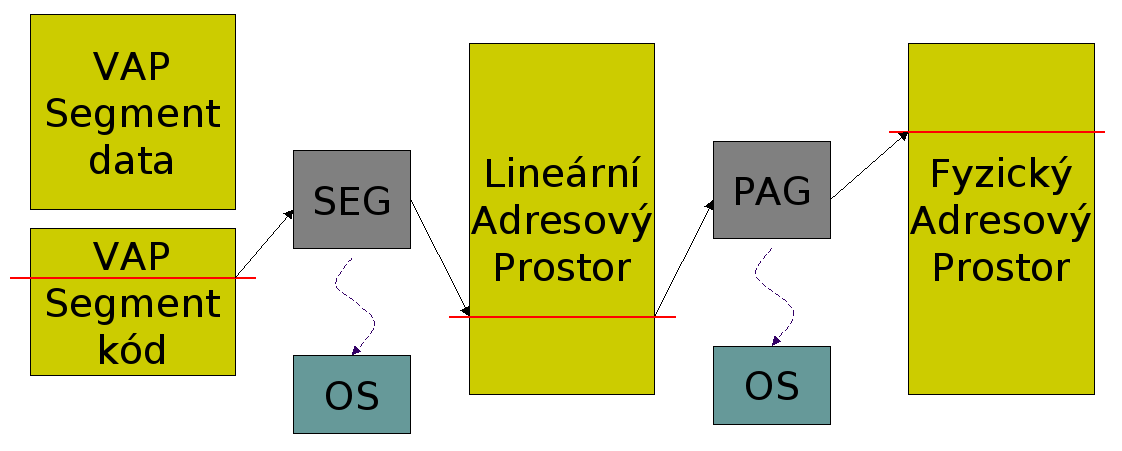
\includegraphics[width=12cm]{informatika/operacne_systemy_a_hw/obrazky/segmentace-a-strankovani.png}\end{center}

\begin{reportN}{Bedn�rek}
T�eba m� p�ekvapila Bedn�kova ot�zka u jedno�rov�ov�ho str�nkov�n�, kdy� se zeptal, co z toho d�l� OS a co procesor (jako co je d�l�no hardwareov� a co softwareov�).
\end{reportN}
\begin{reportN}{Bulej}
Strankovaci tabulku ma kazdy proces vlastni -> ochrana pameti, nemuze pristoupit na cizi stranky (mozna ze to v materialech ke statnicim je, ale ja to z nich nepochopil...)
\end{reportN}
\begin{reportN}{Skopal}
Nejdriv jsem popsal k cemu to je a potom princip. Chtel popsat postup toho co se deje, kdyz se hleda nejaky pointer. Co dela HW, co OS. Pak se zeptal jestli by slo udelat strankovani bez HW podpory (coz rozumne nejde, muselo by se to resit i v prekladacich a bylo by to nefektivni). Pak se zeptal na algoritmy vyhazovani stranek. Popsal jsem FIFO a NRU a to mu stacilo. Na segmentaci nastesti nedoslo.
Celkove velmi prijemne zkouseni. V zasade se spokojil s principy a nestoural moc do detailu.
\end{reportN}
\begin{reportN}{Kofron}
klasika, pre�o, kde, ako ... pre�o to funguje, �o sa rob� pri v�padku str�nky, pre�o dve in�tancie jedn�ho programu nelez� do kapusty aj ke� pracuj� s rovnak�mi virtu�lnymi adresami (ka�d� m� vlastn� str. tabu�ku), tvar adresy, prevody...


ka�d� proces m� vlastn� tabulku, jej� adresa v registru
\end{reportN}
\begin{reportN}{IOI 21. 6. 2011}
Dan� procesor pou��v� 32-bitovou architekturu a dvou�rov�ov� str�nkov�n�.
Instrukce MOV[0x12345678], EAX zapisuje obsah registru EAX na adresu 0x12345678.
Popi�te, jak� operace (p��stupy do registr� a podobn�) vykon�v� p�i prov�d�n� t�to instrukce procesor a jak p�i tom spolupracuje opera�n� syst�m. Rozeberte v�echny mo�n� (z hlediska napln�n� str�nkovac�ch tabulek) p��pady, nepopisujte strategie v�m�ny str�nek.
\end{reportN}

\begin{reportN}{Yaghob} mel ruzn� dotazy, jako proc je str�nka velik� zrovna 4kB, jak je to se str�nkov�n�m na 64-bitov�ch procesorech 
\end{reportN}

\subsection{Syst�my soubor�, adres��ov� struktury}

\begin{e}{Definice}{0}{Syst�my soubor�}
  \begin{pitemize}
    \item Poskytuj� jednotn� rozhran� pro �ten� a ukl�d�n� dat z/do pomocn�ch pam�t�
(sekund�rn�, terci�ln�).
    \item Skr�vaj� povahu za��zen�, na kter�m jsou um�st�ny. Aplikace s t�mto za��zen�m mohou
pracovat pouze p�es rozhran� souborov�ho syst�mu, tedy mohou prov�d�t pouze operace
nad soubory a adres��i. Nemohou ale ��st �i zapisovat p��mo z/do za��zen� pod
souborov�m syst�mem. Pro aplikace nemus� b�t viditeln�, zda je on�m za��zen�m pevn�
disk, n�jak� vzd�len� s�ov� �lo�i�t� �i opera�n� pam� (RAM dsk).Administr�to�i
samoz�ejm� mohou ��st i p��mo ze za��zen�.
    \item Souborov� syst�my se obvykle pou��vaj� na pevn�ch disk�ch, CD/DVD a dal��ch
m�di�ch, kter� neumo��uj� p�istupovat k dat�m p��mo po bajtu (mezi n�mi, ani procesor
to p�i p��stupu do RAM ned�l�), ale po bloc�ch pevn� velikosti � sektorech. Obvykl�
velikost u dne�n�ch pevn�ch disk� je 512 B u CD/DVD jsem vid�l 2 KB. Souborov�
syst�my jsou navr�eny pr�v� tak, aby s takov�mi za��zen�mi efektivn� pracovaly.
    \item \textbf{Velikost blok�}: souborov� syst�my obvykle nepracuj� p��mo se sektory, ale definuj� si
vlastn� bloky, velk� obvykle n�kolik cluster� (4, 8, 16, 32). T�mto blok�m se na Unixu
��k� prost� blocks, na Windows clustery (�esky aloka�n� jednotky). Souborov�
syst�my um� ukl�dat data pouze s granularitou danou velikost� jednoho bloku.
  \begin{pitemize}
    \item P��li� mal� bloky jsou sice �etrn� k pl�tv�n� m�sta �na konci soubor�� (pokud data
souboru skon�� uprost�ed bloku, moc voln�ho m�sta se nevypl�tv� � mal� intern�
fragmentace). Mal�ch blok� mus� b�t ale velk� mno�stv�, aby pokryly celou oblast
m�dia, tak�e intern� datov� struktury (a tedy i �asov� re�ie) jsou v�t��.
    \item Velk� bloky znamenaj� jednodu��� datov� struktury, ale v�t�� intern� fragmentaci
(pl�tv�n� voln�ho m�sta).
  \end{pitemize}
\end{pitemize}  
\end{e}
    \begin{center}
      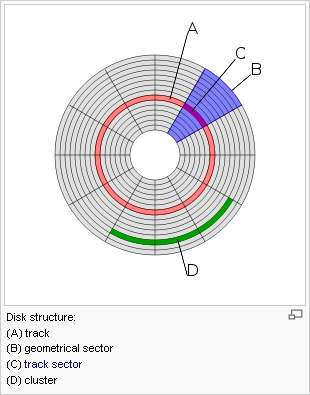
\includegraphics[height=7cm]{informatika/operacne_systemy_a_hw/obrazky/disc.png}
    \end{center}   
\begin{e}{Definice}{0}{soubor}
  Perzistentn� �lo�i�t� dat v pomocn� pam�ti. Ka�d� soubor je obvykle tvo�en
jedn�m nebo v�ce bloky dat, kter� obsahuje, a metadaty s r�zn�mi informacemi.
  \begin{pitemize}
    \item pojmenov�n� souboru (umo��uje u�ivateli p��stup k jeho dat�m;
    p�esn� pravidla pojmenov�n� ur�uje OS - mal� vs. velk� p�smenka,
    speci�ln� znaky, d�lka jm�na, p��pony a jejich v�znam)
    \item atributy soubor� (op�t ur�uje OS) - jm�no, typ, um�st�n�, velikost, ochrana, �asy, vlastn�k, \dots
    \item struktura soubor� - sekvence bajt� / sekvence z�znam� / strom
    \item typy soubor� - b�n� soubory, adres��e (syst�mov� soubory vytv��ej�c� strukturu souborov�ho syst�mu), speci�ln� soubory (znakov�/blokov�, soft linky)
\item \textbf{Operace} - CREATE, OPEN, CLOSE, READ, WRITE, SEEK, DELETE, MAP, UNMAP,
RENAME (nemus� b�t p��tomna, pokud je jm�no souboru ulo�eno jen v jeho
rodi�ovsk�m adres��i, jak tomu je v EXT), LOCK, UNLOCK..
    \item  \textbf{��dk� soubory (sparse files)} - Rozum� se j�m soubor obsahuj�c� velk� shluky nulov�ch bajt�, kter� je v souborov�m syst�mu ulo�en �sporn�m zp�sobem tuto jeho vlastnost vyu��vaj�c�m. To je zaji�t�no tak, �e jsou m�sto velk�ch �d�r� (tj. shluk� nul) na m�dium zaznamen�na pouze stru�n� metadata, v kter�ch je ulo�ena d�lka a pozice d�r. Nenulov� ��sti souboru jsou na m�dium zaps�ny obvykl�m zp�sobem a za pomoci metadat z nich opera�n� syst�m dok�e za b�hu zp�t konstruovat p�vodn� dlouh� soubor vypln�n� mnoha nulami. ��dk� soubory tedy mohou naj�t sv� uplatn�n� nap��klad pro
reprezentaci obraz� disk� virtu�ln�ch po��ta��.
    \begin{center}
      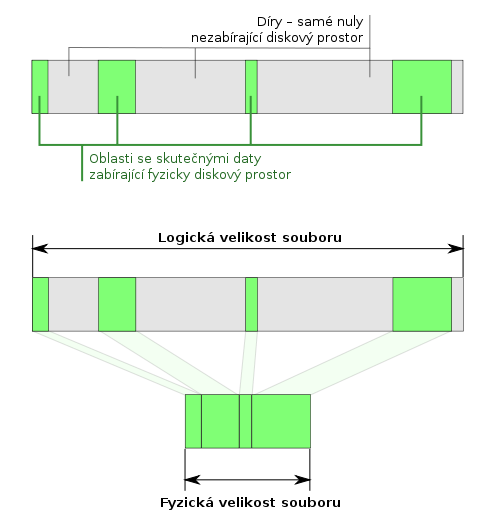
\includegraphics[height=7cm]{informatika/operacne_systemy_a_hw/obrazky/sparse-files.png}
    \end{center}    
  \end{pitemize}
\end{e}



\begin{obecne}{Adres��e}
  \begin{pitemize}
    \item v�t�inou zvl�tn� typ souboru
    \item operace nad adres��i - CREATE, DELETE, LIST, RENAME
    \item ko�en, aktu�ln� adres��, absolutn�/relativn� cesta
    \item hierarchick� struktura 
    \begin{pitemize}
      \item \emph{strom}~-- jednozna�n� pojmenov�n� (cesta)
      \item \emph{DAG}~-- v�cezna�n� pojmenov�n�, ale nejsou cykly
      \item \emph{obecn� graf}~-- cykly vytv��� probl�m p�i prohled�v�n�
    \end{pitemize}
    \item implementace adres��� - z�znamy pevn� velikosti, spojov� seznam, B-stromy 
  \end{pitemize}
\end{obecne}

\begin{obecne}{Co mus� filesyst�m um�t?}
mus� spl�ovat 3 v�ci: 
\begin{pitemize}
\item \emph{spr�vu soubor�} (kde jsou, jak velk�) 
\item \emph{spr�vu adres���} (p�evod jm�no $\leftrightarrow$ id) (n�kdy to d�l� jin� prost�edek, dnes v�t�. um� FS s�m), 
\item \emph{spr�vu voln�ho m�sta}. n�kdy mohou b�t i dal�� (odolnost proti v�padk�m) 
\end{pitemize}
\end{obecne}

\begin{obecne}{Linky}
  \begin{pitemize}
    \item \textbf{Hard link}~-- Na jedna data souboru se odkazuje z r�zn�ch polo�ek v adres���ch (na urovni FS) $\rightarrow$ m�n� FS ze stromu na DAG \footnote{Hard linky se obvykle nepovoluj� vytv��et na adres��e vzhledem k mo�n�mu
vzniku ne��douc�ch kru�nic. Ty jsou ne��douc�, proto�e pak mohou vznikat
entity, u kter�ch nelze po��t�n�m referenc� odhalit, �e mohou b�t smazan�. Je
nutn� pou��t garbage collection.}
\item \textbf{Soft link}~-- Speci�ln� soubor, kter� obsahuje jm�no souboru (na urovni OS)\footnote{Soft Linky mohou odkazovat jak na soubory, tak na adres��e. Proto�e se jedn� pouze o
jmenn� aliasy (nepropojuj� se samotn� objekty), ani vznik kru�nic neznamen�
��dn� probl�my.}
  \end{pitemize}
\end{obecne}

\begin{obecne}{MBR} 
A master boot record (MBR) is a type of boot sector. It consists of a sequence of 512 bytes located at the first sector of a data storage device such as a hard disk. May be used for one or more of the following:
  \begin{pitemize}
    \item Holding a partition table which describes the partitions of a storage device. In this context the boot sector may also be known as a partition sector.
    \item Bootstrapping an operating system. The BIOS built into a PC-compatible computer loads the MBR from the storage device and passes execution to machine code instructions at the beginning of the MBR.
    \item Uniquely identifying individual disk media, with a 32-bit disk signature, even though it may never be used by the operating system.
  \end{pitemize}
\end{obecne}


\begin{obecne}{FAT} 
  \begin{pitemize}
    \item System souboru FAT rozdeluje disk na dve vyznacne casti - samotnou tabulku FAT (ta je zpravidla ve dvou kopiich) a datovou oblast. Datova oblast je rozdelena na clustery (napriklad po 4096 bajtech) a FAT tabulka ma tolik polozek, kolik ma datova oblast clusteru (1:1).
    \item \textbf{FAT tabulka}~-- pole z�znam�\footnote{12 bitov�ch na FAT12, 16 bitov�ch
na FAT16, 32 bitov�ch na FAT32}, obsahuje �islo dalsiho clusteru v �ad� nebo speci�ln� z�znamy (ozna�en� end of clusterchain, bad cluster, reserved cluster a free cluster)
    \item \textbf{Alokace souboru}~-- jednosm�rn� spojov� seznam, ka�d� blok ukazuje na dal�� p�es FAT tabulku    
    \begin{center}
      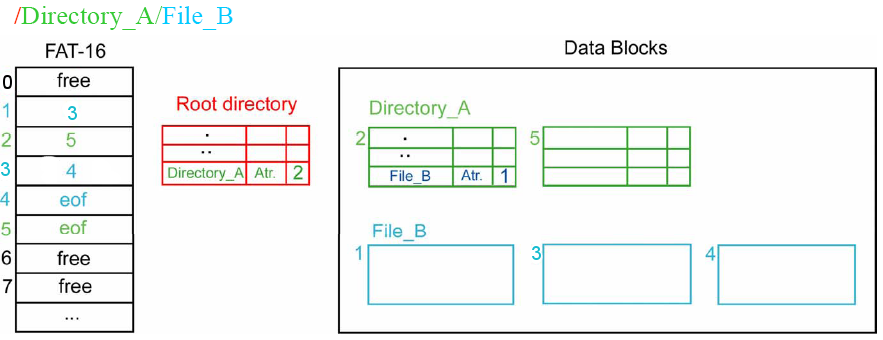
\includegraphics[height=5cm]{informatika/operacne_systemy_a_hw/obrazky/FAT16.png}
    \end{center}      
    \subitem - Kdyz je nejaky cluster volny, v prislusne polozce FAT je 0. Tedy 
kdyz chci najit volne misto, tak staci najit libovolnou polozku FAT, 
ktera je 0, odpovidajici cluster pak je volny.    
    \item Adresare i soubory jsou ulozeny stejne. Rozdily mezi adresari a soubory (krom daneho atributu) neexistuji. Z hlediska ulozeni na disku je adresar proste soubor, jehoz obsahem jsou adresarove polozky. Vyjimka viz root adresar. 
    \item \textbf{Root adres��}~-- V root adresari, i ve vsech ostatnich adresarich, jsou 
proste jen za sebou ulozeny polozky. Kazda polozka obsahuje jmeno 
souboru nebo adresare, ke kteremu se vztahuje, atributy rozlisujici 
napriklad prave adresare od souboru, delku, prvni cluster, atd.
    \subitem - Root directory ma pevnou velikost ve FAT 12/16
    \subitem - Polozky root adresare, ktere nejsou pouzite, jsou oznacene jako prazdne 
(ale porad patri do root adresare, aby velikost zustala konstantni). 
Pridani pak pouzije nekterou prazdnou polozku. Pokud jsou jiz vsechny 
polozky plne, dalsi nelze pridat.
    \item \textbf{Vyhled�v�n� souboru}~--  Postupne ... v root adresari se najde prvni podadresar cesty, v nem se 
najde druhy a tak dale. (tzn. line�rn� struktura)
    \item Adresarova struktura je ulozena prave v jednotlivych adresarich. 
Napriklad, pokud je na disku soubor 
\\$C:\backslash FOO\backslash BAR\backslash SOUBOR.TXT$, tak v korenovem 
adresari bude polozka FOO s atributem indikujicim, ze se jedna o adresar 
a s cislem prvniho clusteru adresare FOO, rekneme ze 123. V clusteru 123 
pak budou polozky adresare FOO, mezi nimi bude podobne polozka BAR pro 
adresar BAR a cislem prvniho clusteru adresare BAR, rekneme 456. A v 
clusteru 456 budou polozky adresare BAR, mezi kterymi bude i polozka 
SOUBOR.TXT ...
    \item dnes se ni setkame je�t� na flashk�ch a pam�ov�ch kart�ch                
    \item \textbf{nevyhody FAT}: 
    \subitem - velikost souboru max 4 GB  
    \subitem - svazky - FAT32 re�ln� okolo 8TB (32kB clustery), nem� ale ochranu proti fragmentaci
    \subitem - pr�va - None of the various FAT-flavours has facilities for user-based access restrictions.
    \item \url{https://d3s.mff.cuni.cz/pipermail/osy/2005-June/000167.html}
    \item \url{http://en.wikipedia.org/wiki/File_Allocation_Table}
\end{pitemize}
\end{obecne}

\begin{obecne}{NTFS} 
  \begin{pitemize}
    \item Zase rozd�luje odd�l na dv� ��sti tabulka MFT (jako soubor, ma ale p�i�azenou pr�zdnou oblast aby se p�i r�stu nefragmentovala) a datovou oblast.
    \item \textbf{Metafiles} - prvn�ch cca 16 souboru jsou tzv. Metafiles, ka�d� se star� o n�co $\Rightarrow$ flexibilita nap�. pri poskozenem povrchu        
    \subitem p��klady souboru: \$MFT, \$MFTmirr (MFT a zalozni kopie uprostred disku),\$LogFile (zurnalovaci soubor),\$. (root directory),\$Bitmap (bitove pole volneho mista) atd...             
    \item \textbf{�urn�l} -- Operace s diskem se provadeji jako Transakce, tak�e nap�. pokud pri zapisu souboru FS zjisti ze cluster je fyz. vadn�, celou trasakci rollbackuje a pusti ji jinde znovu.
    \item Dal�� vlastnosti ktere ma navic: sifrovani, komprese, hardlinky (soubor je fyz. na disku jednou a ma vic zaznamu v MFT)
    \item \textbf{MFT tabulka} -- obdoba FAT, vsechna metadata o souborech (jmeno,datum,prava) jsou ulozena v MFT - omoznuje pridavat ficury, muze obsahovat primo i male soubory nebo odkazy na clustery (za��naj�c� cluster + po�et)\footnote{tzv. run listy}
    \begin{center}
      \includegraphics[height=5cm]{informatika/operacne_systemy_a_hw/obrazky/mft-entry-extent.gif}
    \end{center}     
    \item Vnit�n� struktura adres��e se realizuje B+Stromem (lexikograficky setrideny) zase pokud je malej zustane v MFT pokud je vetsi je v clusteru a v MFT je jenom ko�enov� ��st B+Stromu.     
    \begin{center}
      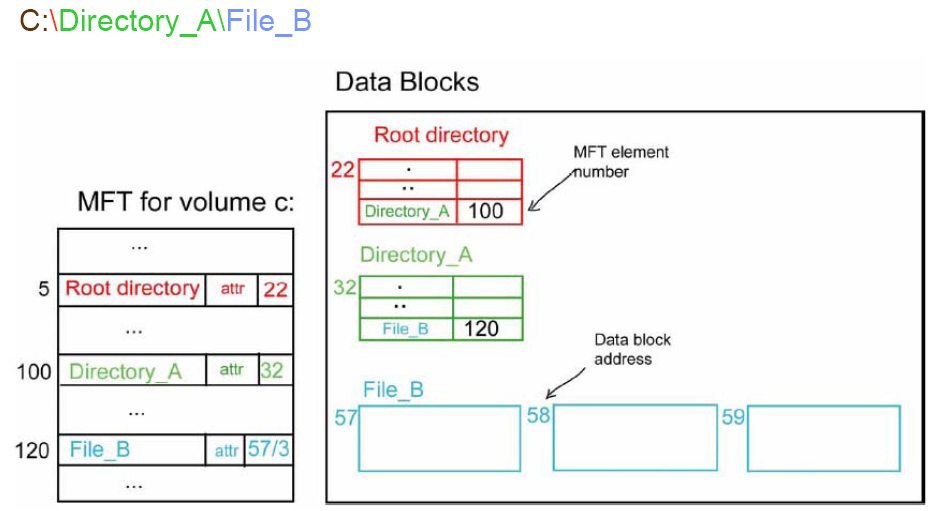
\includegraphics[height=5cm]{informatika/operacne_systemy_a_hw/obrazky/ntfs.png}
    \end{center}           
    \item \url{http://pages.cs.wisc.edu/~bart/537/lecturenotes/s26.html}    
    \item \url{http://www.digit-life.com/articles/ntfs/}
    \item \url{http://www.pcguide.com/ref/hdd/file/ntfs/archSector-c.html}
    \item \url{http://cs.wikipedia.org/wiki/NTFS}    
    \item \url{http://ixbtlabs.com/articles/ntfs/}
    \end{pitemize}
    
\end{obecne}

\begin{obecne}{ext2} 
  \begin{pitemize} 
    \item Prostor je u ext2 rozd�len do blok�, ty jsou rozd�leny do skupin (Block Groups) typicky jeden soubor se dr�� v jedn� skupin� (redukce fragmentace). Ka�d� skupina obsahuje kopii superbloku (obsahuje kritick� informace pro boot systemu) a Group Descriptors Table\footnote{ Early versions of the ext2 file system to make copies of the superblock at the beginning of each block group. This led to heavy losses of disk space, so that later the number of backups superblock has been reduced, and for their placement have been allocated a group of blocks 0, 1, 3, 5 and 7.}, bitmapu datov�ch blok�, bitmapu inodes, Inode tabulku a nakonec datov� bloky. 
    \begin{center}
      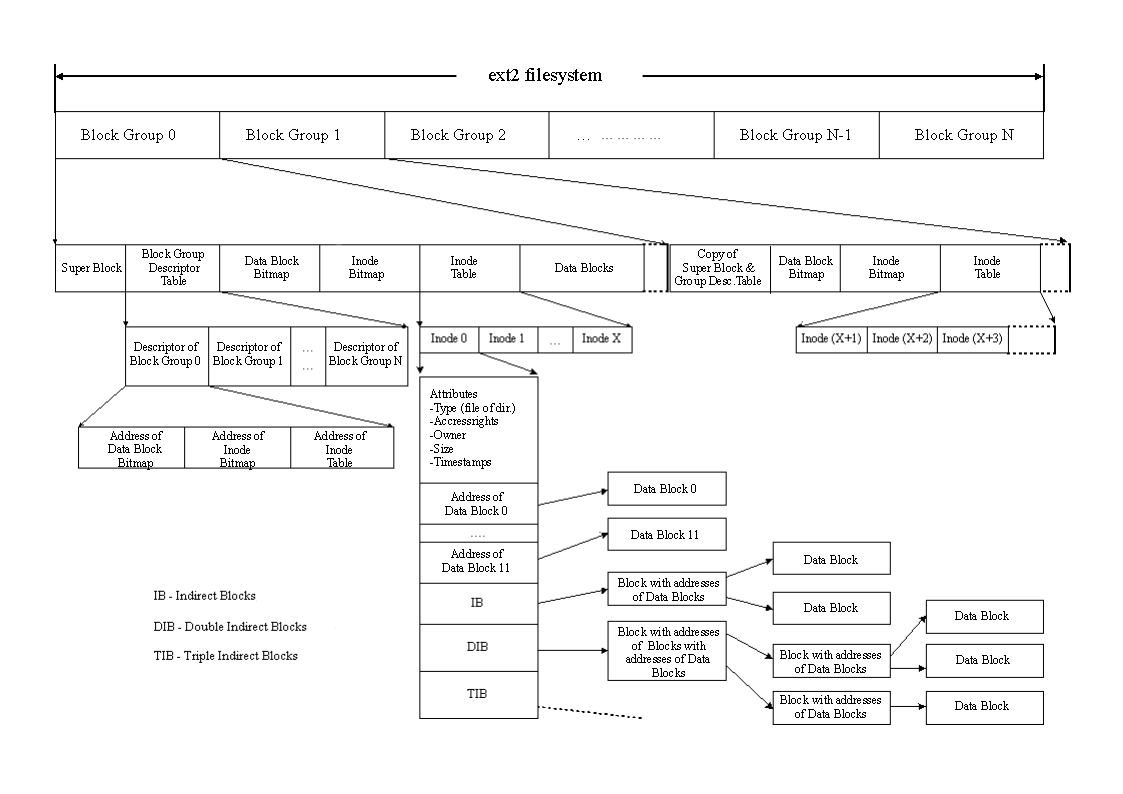
\includegraphics[height=13cm]{informatika/operacne_systemy_a_hw/obrazky/ext2-all.png}
    \end{center}     
    \item \textbf{inode} -- ka�d� soubor nebo slo�ka (zde tak� soubor) je reprezentov�na jako inode (v inode tabulce), obsahuje pr�va, velikost a hlavn� pointery na datov� bloky (12pointer� na p��m� odkaz a dal�� na stromovou strukturu), slo�ky
obsahuj� v datov�ch bloc�ch linked list inodes kter� obsahuj� a jejich n�zvy (samotn� inode n�zev souboru neobsahuje!)        
    \item Proc se porad pouziva - kv�li rychlosti
    \item �urn�lov�n� zavedeno u ext3              
    \item \url{http://www.nongnu.org/ext2-doc/ext2.pdf}
    \item \url{http://homepage.smc.edu/morgan_david/cs40/analyze-ext2.htm}    
    \item \url{http://www.science.unitn.it/~fiorella/guidelinux/tlk/node95.html}

    \end{pitemize}
    
\end{obecne}
\begin{obecne}{Shrnut�}
\\
\begin{tabular}{| 1 | p{4cm} | p{4cm} | p{4cm} | p{4cm} | }
\hline          
    & spr�va soubor� & spr�va adres��� & spr�va voln�ho m�sta & dal�� \\
\hline           
\hline             
  FAT & line�rn� spojov� seznam (p�es FAT) & neset��d�n� pole & v FAT, d� se ��ct bitmapa & neum� nic pokro�il�ho: linky, zabezpe�en�,relokaci po�kozen�ch cluster�...  \\
\hline            
  NTFS & runlisty (odkazy na clustery jsou v MFT) & B*strom (neredundatn�) & bitmapa & kv�ty, zabezp., transakce, linky, relokace soubor�, �ifrov�n�, ��dk� soubory \\
\hline            
  ext2 & index(12+3 pointery), ext4�runlist & linked list, ext4�2-level hashing & bitmapy & zabezpe�en�, linky, v z�kladu neum� kompresi a �ifrov�n�\\
\hline  
\end{tabular}
\end{obecne}
\begin{obecne}{Algoritmy pln�n� po�adavk� disku}
\begin{pitemize}
\item Disk o struktu�e souborov�ho syst�mu nic nev�, dost�v� pouze po�adavky na z�pis �i �ten� blok� dat z ur�it�ch m�st.
\item \textbf{Shortest seek first} (z nevy��zen�ch po�adavk� na �ten�/z�pis dat beru ty, kter� jsou
nejbl�e aktu�ln� pozici hlavy, tedy maj� nejmen�� d�lku posunu (seek), tedy nejni���
seek time. Probl�m je, �e n�kter� po�adavky tak nemus�m obslou�it v�bec (nap��klad
mi po��d p�ich�z� po�adavky �ten� n�kde uprost�ed disku, a tak se po��d pohybuju
tam... ale p�r po�adavk� na �ten� okraj� disku tedy v�bec nevy��d�m, proto�e je tam
dlouh� seek).
\item \textbf{V�tah (elevator)}. Obsluhuji po�adavky pouze v jednom �sm�ru,� t�m se nap��klad
st�le vzdaluji od st�edu disku. Jakmile v dan�m sm�ru nejsou ji� ��dn� po�adavky na
vy��zen�, obr�t�m sm�r a zase pomalu sm��uju ke st�edu disku).
\item \textbf{jednosm�rn� v�tah} (po��d jezd� jedn�m sm�rem, v�dy na konci se posune na nejni���
cylindr s po�adavkem).
  \end{pitemize}
\end{obecne}

\begin{obecne}{RAID (Redundant Array of Inexpensive Disks)}
  \begin{pitemize}
    \item JBOD (Just a Bunch of Disks)
    \item RAID 0~-- striping, ��dn� redundance
    \item RAID 1~-- mirroring, redundance
    \item RAID 0+1~-- mirroring a striping
    \item RAID 2~-- 7-bitov� paritn� Hamming�v k�d
    \item RAID 3~-- 1 paritn� disk, po bitech na disky
    \item RAID 4~-- 1 paritn� disk a striping
    \item RAID 5~-- distribuovan� parita a striping
    \item RAID 6~-- distribuovan� parita -- dvojit� P+Q, striping 
  \end{pitemize}
\end{obecne}
\begin{obecne}{Zdroje:}
  \begin{pitemize}
    \item http://www.jadro-windows.cz/
  \end{pitemize}    
\end{obecne}
\begin{reportN}{Galambo�} inode\end{reportN}
\begin{reportN}{Galambo�} Konkretni soubory system NTFS - tady jsem popletl jak vlastne pracuje FATka, o NTFS jsem mel tak jako povesechne informace, proste nic moc jsem nevedel, ale zase jsme si popovidali, byly mi vysvetleny me omyly a nakonec oka. 
Jinak je pravda, ze toho chce docela hodne a dopodrobna, ale kdyz clovek rekne, ze proste k tomuhle vic nesehnal a ze podrobnosti proste nevi, pobavi se o tom s Vami a vetsinou se to da dokupy. 
\end{reportN}
\begin{reportN}{Skopal} Zkou�el s�m p. Skopal a jeliko� jsem se FS u�il jako jednu z prvn�ch ot�zek, v n�valu dal��ch informac� jsem toho mezit�m dost zapomn�l. Popsal jsem jeden a p�l strany obecn�mi vlastnostmi FS, co to je soubor, adres�� atd. Popsal jsem FAT, NTFS a ext2, a to dost stru�n�. Obecn� vlastnosti ho nezaj�maly, hned p�e�el k FAT a jej�m nev�hod�m, ot�zky byly rychl� a dost podrobn�, bylo vid�t, �e to se mnou nebude m�t jednoduch�. Pak m�l ot�zky na NTFS, co m� za spec. soubory, kde�e je v syst�mu implementov�n B-strom atd. K ext2 jsme se nedostali a� na jedinou zm�nku, a to je alokace soubor� (ve FAT line�rn� struktura, v ext2 strom). Kdy� polo�il ot�zku na B-stromy v NTFS a po moj� t�ce nejist� odpov�di prohl�sil, �e mu to sta�� a ode�el, bylo mi jasn�, �e tohle nedopadne dob�e.
\end{reportN}
\begin{reportN}{Yaghob} Konkretni Filesystemy - no jeste pred dvema dny by to byla moje smrt, nastesti sem se na to vcera zameril a nasel si opravdu presne jak funguje FAT, NTFS a ext2. Nakonec z toho byly tri papiry, az jsem na sebe byl pysny U FAT bylo treba napsat, jak se to alokuje, jak vypada ta tabulka, jakou roli ma kor. adresar, jak jsou tam ulozeny adresare, soubory apod. U NTFS jsem popsal vlastnosti ktere to ma navic, jako zurnal, sifrovani a pak rozepsal MFT docela podrobne, zase jak se resi soubory, adresare. Veci jako jak jsou tam ulozeny jednotlivy volume, MBR atd po me nastesti nechtel U ext2 je asi dulezite pochopit jak ten inode funguje, jak je to tam ve skupinach bloku, co je to superblok. Prislo mi, ze hlavni duraz je kladeny na to, at se vi, jak jsou tam ulozeny adresare a soubory. Pak prislo par otazek typu, jake jsou omezeni FATky, (velikost souboru, partitiony, ale hlavne se po me chtelo slyset: prava), kde se s tim dnes setkame (flashky, pametove karty) - na ty jsem dosel po vyjmenovani win98, mobilu, zkusil jsem i routery a ind. pocitace a nakonec me uspesne dovedl ke spravne odpovedi U ext2 prislo, proc se to porad jeste pouziva,kdyz je to tak stary FS - jedine co me napadlo byla rychlost - spravne
\end{reportN}

\subsection{Bezpe�nost, autentizace, autorizace, p��stupov� pr�va\footnote{z
p�edn�ek ZOS(Yaghob) a OI1(Bene�)}}

\begin{e}{Definice}{0}{0}
  \begin{pitemize}
    \item \textbf{Ochrana}~-- s prost�edky OS mohou pracovat pouze autorizovan� procesy
    \item \textbf{Autorizace}~-- zji�t�n� opr�vn�nosti po�adavku
    \item \textbf{Bezpe�nost}~-- zabra�uje neautorizovan� p��stup do syst�mu
    \item \textbf{P�istupov� pr�vo}~-- povolen�/zak�z�n� vykon�vat n�jakou operaci
    \item \textbf{Dom�na ochrany}~-- uchov�n�n� autorizac�, mno�ina p�r� (objekt:pr�va)
    \begin{pitemize}
      \item \textbf{ACL (Access Control List)}~-- ke ka�d�mu objektu seznam pr�v pro u�ivatele/skupiny
      \item \textbf{C-list (Capability List)}~-- ke ka�d�mu u�ivateli/skupin� seznam pr�v pro objekty

      \item \textbf{ACM (Access Control Matrix)}~-- ��dky matice odpov�daj� u�ivatel�m, sloupce objekt�m. V pol��ku dan�m ��dkem a sloupcem je z�znam o �rovni opr�vn�n� odpov�daj�c�ho u�ivatele k p��slu�n�mu objektu. P��stupov� matice je zpravidla velmi velk� z�le�itost, zhusta ��dk�.
    \end{pitemize}
  \end{pitemize}
\end{e}

  \begin{figure}[!ht]
    \begin{center}
      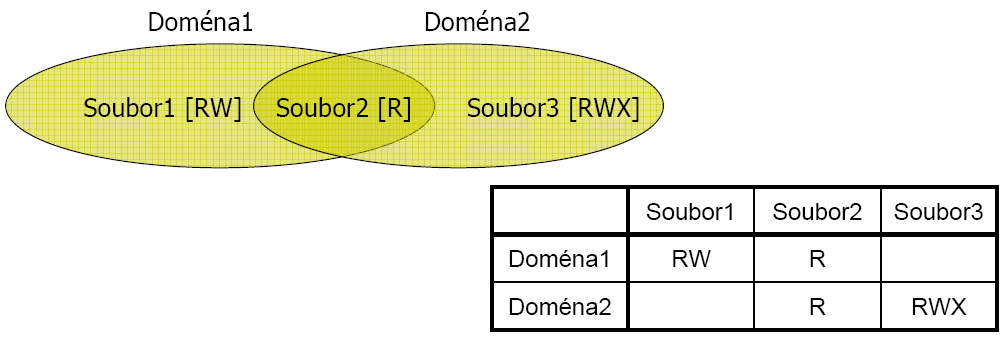
\includegraphics{informatika/siete_a_bezpecnost/obrazky/domeny-ochrany.png}
      \caption{Dom�ny ochrany}
    \end{center}
  \end{figure}
\subsubsection*{Bezpe�nost}

\begin{obecne}{Bezpe�nostn� modely obecn�}
Prvn� f�z� tvorby bezpe�n�ho IS je volba vhodn�ho bezpe�nostn�ho modelu.
Z�kladn� po�adavky bezpe�nosti: utajen�, integrita, dostupnost, anonymita.
P�edpokl�dejme, �e um�me rozhodnout, zda dan�mu subjektu poskytnout
p��stup k po�adovan�mu objektu. Modely poskytuj� pouze mechanismus pro
rozhodov�n�!
  \begin{pitemize}
      \item \textbf{Jedno�rov�ov� modely} jsou vhodn� pro p��pady, kdy sta�� jednoduch�
ano/ne rozhodov�n�, zda dan�mu subjektu poskytnout p��stup k po�adovan�mu
objektu a nen� nutn� pracovat s klasifikac� dat.
      \item \textbf{V�ce�rov�ov� modely} - M��e existovat n�kolik stup�� senzitivity
a "opr�vn�nosti". Tyto stupn� senzitivity se daj� pou��t k algoritmick�mu rozhodov�n� o p��stupu dan�ho subjektu k c�lov�mu objektu,
ale tak� k ��zen� zach�zen� s objekty. V�ce�rov�ov� syst�m "rozum�"
senzitivit� dat a ch�pe, �e s nimi mus� zach�zet v souladu s po�adavky
kladen�mi na dan� stupe� senzitivity. Rozhodnut� o p��stupu pak
nezahrnuje pouze prov��en� �adatele, ale t� klasifikaci prost�ed�, ze
kter�ho je p��stup po�adov�n.
  \end{pitemize}
\end{obecne}  
\begin{obecne}{Bezpe�nost fyzick� p�enosov� vrstvy}
Bezpe�nost je do ur�it� m�ry z�visl� na pou�it�m p�enosov�m m�diu. �tok
proti komunika�n�m link�m m��e b�t pasivn� (pouze odposlech), nebo ak-
tivn� (vkl�d�n� dal��ch informac� do komunikace).
\end{obecne}

\begin{obecne}{V�ce�rov�ov� bezpe�nost v DB\footnote{zdroj: vypracovan� ot�zky
na zkou�ku z OI1}}
  \begin{pitemize}
      \item \textbf{partitioning} - Datab�ze je rozd�lena dle stupn� citlivosti
informac� na n�kolik subdatab�z�, co� vede ke zv��en� redundance s
n�slednou zt�enou aktualizac� a ne�e�� probl�m nutnosti sou�asn�ho
p��stupu k objekt�m s r�zn�m stupn�m utajen�.
      \item \textbf{�ifrov�n�} - Senzitivn� data jsou chr�n�na �ifrov�n�m p�ed n�hodn�m
vyzrazen�m. Zn�-li �to�n�k dom�nu dan�ho atributu, m��e snadno
prov�st chosen plaintext attack (utocnik muze ukladat plaintexty podle sveho
vyberu a prohlizet si ciphertexty).
T�ko toti� n�koho zbav�me znalosti �ifrovac�ho kl��e. �e�en�m je pou��vat
jin� kl�� pro ka�d� z�znam, co� je v�ak pom�rn� n�ro�n�. V ka�d�m
p��pad� nutnost neust�l�ho de�ifrov�n� sni�uje v�kon syst�mu.
      \item \textbf{Integrity lock} - Ka�d� polo�ka v datab�zi se skl�d� ze t�� ��st�: $< vlastn� data : klasifikace : checksum >$. 
Vlastn� data jsou ulo�ena v
otev�en� form�. Klasifikace mus� b�t nepad�lateln�, nep�enositeln� a
skryt�, tak aby �to�n�k nemohl vytvo�it, okop�rovat ani zjistit klasifikaci dan�ho objektu. Checksum zaji��uje sv�z�n� klasifikace s daty
a integritu vlastn�ch dat. Model byl navr�en jako dopln�k (access
controller) komer�n�ho S�BD, kter� m�l zajistit bezpe�nost cel�ho
syst�mu. �ed� oblast na obr�zku vyzna�uje bezpe�nostn� perimetr
syst�mu. Access controller nevid� na v�stup datab�ze a nen� schopen
zajistit, na v�stupu ozna�ovala data stupn�m senzitivity.

  \begin{figure}[!ht]
    \begin{center}
      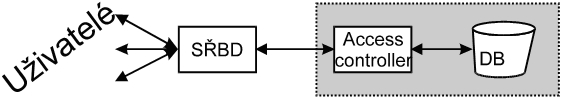
\includegraphics[scale=1.5]{informatika/siete_a_bezpecnost/obrazky/access-controller.png}
      \caption{Access Controller}
    \end{center}
  \end{figure}

      \item \textbf{Spolehliv� front-end (guard)} - Syst�m je op�t zam��len jako dopln�k komer�n�ch S�BD, kter� nemaj� implementov�nu bezpe�nost.
U�ivatel se autentizuje spolehliv�mu front-endu, kter� od n�ho p�eb�r�
dotazy, prov�d� kontrolu autorizace u�ivatele pro po�adovan� data,
p�ed�v� dotazy k vy��zen� S�BD a na z�v�r prov�d� testy integrity
a klasifikace v�sledk� p�ed p�ed�n�m u�ivateli. S�BD p�istupuje k
dat�m prost�ednictv�m spolehliv�ho access controlleru.
  \begin{figure}[!ht]
    \begin{center}
      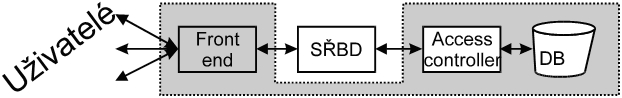
\includegraphics[scale=1.5]{informatika/siete_a_bezpecnost/obrazky/frontend.png}
      \caption{Spolehliv� front-end}
    \end{center}
  \end{figure}
      \item \textbf{Commutative Filter} -- Jde o proces, kter� p�eb�r�
�lohu rozhran� mezi u�ivatelem a S�BD. Filtr p�ij�m� u�ivatelovy
dotazy, prov�d� jejich p�eformulov�n� a upraven� dotazy pos�l� S�BD
k vy��zen�. Z v�sledk�, kter� S�BD vr�t�, odstran� data, ke kter�m
u�ivatel nem� p��stupov� pr�va a takto upraven� v�sledky p�ed�v�
u�ivateli. Filtr je mo�no pou��t k ochran� na �rovni z�znam�, atribut�
a jednotliv�ch polo�ek. V r�mci p�eformulov�n� dotazu m��e nap�.
vkl�dat dal�� podm�nky do dotazu, kter� zajist�, �e v�sledek dotazu
z�vis� jen na informac�ch, ke kter�m m� u�ivatel p��stup.
      \item \textbf{View} - Pohled je ��st datab�ze, obsahuj�c� pouze data, ke
kter�m m� dan� u�ivatel p��stup. Pohled m��e obsahovat i z�znamy
nebo atributy, kter� se v p�vodn� datab�zi nevyskytuj� a vznikly n�jakou
funkc� z informac� p�vodn� datab�ze. Pohled je generov�n dynamicky,
prom�taj� se tedy do n�ho zm�ny p�vodn� DB. U�ivatel klade dotazy
pouze proti sv�mu pohledu - nem��e doj�t ke kompromitaci informac�, ke kter�m nem� p��stup. Z�znam / atribut p�vodn� datab�ze
je sou��st� pohledu, pokud alespo� jedna polo�ka z tohoto z�znamu
/ atributu je pro u�ivatele viditeln�, ostatn� polo�ky v tomto jsou
ozna�eny za nedefinovan�. U�ivatel p�i formulov�n� dotazu m��e pou��vat
pouze omezenou sadu povolen�ch funkc�. Tato metoda je ji� n�vrhem
sm��uj�c�m k vytvo�en� bezpe�n�ho S�BD.
  \end{pitemize}
\end{obecne}

\subsubsection*{Autentizace}
  Identifikace n���m, co u�ivatel v�, m� nebo je. 
  \begin{pitemize}
    \item \textbf{Hesla}
    \begin{pitemize}
      \item slovn�kov� �tok (80--90\% hesel je jednoduch�ch), hrub� s�la
      \item vynucov�n� d�lky a slo�itosti hesla
    \end{pitemize}
    \item \textbf{Model ot�zka/odpov��} (challenge-response) -- nap�. autentizace po��ta��. Po��ta�, kter� se
chce autentizovat obdr�� n�hodn� dotaz, kter� zpracuje (nap�. za�ifruje
tajn�m kl��em) a ode�le v�sledek. V�sledek je ov��en a pokud je spr�vn�,
autentizace je uskute�n�na. 
    \item \textbf{Fyzick� objekt}~-- smartcards, USB kl��e (certifik�ty)
    \item \textbf{Biometrika}~-- otisky prst�, rohovka, hlas
  \end{pitemize}

\begin{obecne}{Autentizace v prost�ed� datab�ze}
Ka�d�, komu je povolen p��stup k datab�zi, mus� b�t pozitivn� identifikov�n.
datab�ze pot�ebuje p�esn� v�d�t, komu odpov�d�. Proto�e v�ak zpravidla b��
jako u�ivatelsk� proces, nem� spolehliv� spojen� s j�drem OS a tedy mus�
prov�d�t vlastn� autentizaci.
\end{obecne}
\begin{obecne}{Autentizace v s�ti}
Proto�e s�t'ov� prost�ed� zpravidla nen� pova�ov�no za bezpe�n�, je t�eba
vyu��vat autentiza�n� mechanismy odoln� v��i odposlechu, resp. aktivn�m utok�m. �asto b�v� ��douc� �e�it jednotn� p�ihl�en� (single sign on). S procesem integrace autentiza�n�ch mechanism� souvis� nutnost zaveden�
centr�ln� spr�vy u�ivatel� nebo alespo� synchronizace z�znam� o u�ivatel�ch.
\end{obecne}
\subsubsection*{Autorizace}
Existuj� r�zn� �rovn� ochrany objektu:
\begin{enumerate}
    \item \textbf{��dn� ochrana} - Je nutna alespon samovoln� casov� separace proces�.
    \item \textbf{Izolace} - Procesy o sobe v�bec nev� a syst�m zajis�uje ukryt� objekt�
p�ed ostatn�mi procesy.
    \item \textbf{Sd�len� vseho nebo niceho} - Vlastn�k objektu deklaruje, zda je objekt
public nebo private (tedy jen pro neho).
    \item \textbf{Sd�len� s omezen�mi pr�stupy} - OS testuje opr�vn�nost ka�d�ho pr�stupu
k objektu. U subjektu i objektu existuje z�znam, zda m� subjekt pr�vo
pr�stupu k objektu.
    \item \textbf{Sd�len� podle zp�sobilosti} - roz���en� p�edchoz�ho - Opr�vnen� dynamicky z�vis� na aktu�ln�m kontextu.
    \item \textbf{Limitovan� pouzit� objekt�} - Krome opr�vnen� pr�stupu specifikujeme,
jak� operace sm� subjekt s objektem prov�det.
\end{enumerate}

TODO: p��stupov� pr�va
???
Ochrana informace I.

\subsection{Druhy �tok� a obrana proti nim}

\subsubsection*{Vnit�n� �toky}
\begin{pitemize}
  \item \textbf{Trojsk� k��}~-- zd�nliv� ne�kodn� program obsahuje \uv{zl�} k�d
  \item \textbf{Login spoofing}~-- fale�n� \uv{logovac�} obrazovka
  \item \textbf{Logick� bomba}~-- zam�stnanec vprav� kus k�du do syst�mu, kter�
  mus� b�t pravideln� informov�n o tom, �e zam�stnanec je st�le zam�stnancem
  \item \textbf{Zadn� dv��ka (trap door, back door)}~-- k�d p�i n�jak� podm�nce
  p�esko�� norm�ln� kontroly
  \item \textbf{P�ete�en� vyrovn�vac� pam�ti (buffer overflow)}
  \begin{pitemize}
    \item ve velk�m mno�stv� k�du nejsou d�l�ny kontroly na p�ete�en� pol� pevn� velikosti
    \item p�i p�ete�en� se typicky p�ep�e ��st z�sobn�ku a lze tam um�stit adresu k�du i samotn� k�d, kter� se vykon� p�i n�vratu z funkce
  \end{pitemize}
\end{pitemize}

\subsubsection*{Vn�j�� �toky}
\begin{pitemize}
  \item \textbf{Virus}~-- vytvo�� se naka�en� \uv{��dan�} soubor
  \item \textbf{Internetov� �erv (worm)}~-- samoreplikuj�c� se program (�erv),
  vyu��v� n�jak� chyby syst�mu 
  \item \textbf{Mobiln� k�d}~-- applety, agenti\dots
\end{pitemize}

\subsubsection*{�to�n�ci}
�to�n�kem m��e b�t bu� n�hodn� u�ivatel, vnit�n� pracovn�k, zlo�inec (zven��) nebo �pion (vojensk�, komer�n�). C�le �tok� jsou na d�v�rnost -- zji�t�n� obsahu, nebo celistvost -- zm�na obsahu, p��padn� dostupnost slu�by -- Denial of service. Ke ztr�t� dat m��e doj�t i v d�sledku chyby hardware, software, lidsk� chyby nebo Bo��ho z�sahu.

\subsubsection*{Obrana}
jsou to sp� banality, ale nic v�c po n�s necht�j�???
\begin{pitemize}
    \item proti trojan�m, backdoor�m, logical bomb -- omezen� p��stupov�ch pr�v, metoda \uv{least privilege}
    \item proti login-spoofu -- \uv{secure attention key}, tj. takov� to \uv{Za�n�te stisknut�m Ctrl-Alt-Del}
    \item proti buffer overflow -- jedin� patche
    \item proti vir�m -- antivirus ;-), anti-spyware 
    \item proti �erv�m -- firewall, patche (�toky jsou v�t�inou proti zn�m�m a opraven�m chyb�m aplikac�, proti druh�mu typu, tzv. \uv{zero-day attack} je jedinou obranou firewall)
    \item proti probl�m�m s aplety a skripty -- sandboxing (b�h v omezen�m prost�ed� bez mo�nosti p��stupu k po��ta�i)
    \item proti v�emu -- backupy ;-)
\end{pitemize}

\subsection{Kryptografické algoritmy a protokoly}

\begin{obecne}{Cíle kryptografie}
  \begin{pitemize}
    \item důvěrnost dat
    \item celistvost dat
    \item autentifikace~-- od koho jsou data
    \item nepopiratelnost~-- když jednou něco potvrdím, nemohu to popřít.
  \end{pitemize}
\end{obecne}

\begin{definiceN}{Kryptografický systém}
 \textbf{ Kryptografický systém} obsahuje:
  \begin{pitemize}
    \item prostor zpráv~-- \emph{plaintext},
    \item prostor šifrovaných zpráv~-- \emph{ciphertext},
    \item prostory šifrovacích a dešifrovacích \emph{klíčů},
    \item efektivní algoritmus pro \emph{generování klíčů},
    \item efektivní algoritmus pro \emph{šifrování},
    \item efektivní algoritmus pro \emph{dešifrování}.
  \end{pitemize}
\end{definiceN}

\begin{definiceN}{označení}
  $C$~-- šifra, $P$~-- otevřený text, $K$~-- klíč,\\
  $\mathbf{E}$~-- šifrovací algoritmus, $\mathbf{D}$~-- dešifrovací algoritmus.\\[3mm]
  \emph{Šifrování:} $C = \mathbf{E}(P)$, resp. $C = \mathbf{E}(K, P)$\\
  \emph{Dešifrování:} $P = \mathbf{D}(C)$, resp. $P = \mathbf{D}(K, C)$\\
\end{definiceN}


\begin{obecne}{Kerchoffovy principy dobrého krypt. systému}
\begin{pitemize}
    \item E a D neobs. tajnou část
    \item E distribuuje rozumné zprávy rovnoměrně po C
    \item se správným klíčem jsou E \& D efektivní
    \item bez správného klíče je dešifrování minimáně NP-úplné. 
\end{pitemize}
\end{obecne}

\begin{obecne}{dělení kryptografických systémů}
\begin{pitemize}
    \item symetrické krypt. systémy : $k = k'$
    \item asymetrické : $k \neq k'$ ( veřejný a tajný klíč ). 
\end{pitemize}
\end{obecne}

\begin{obecne}{Model útočníka podle Doleva a Yao}
\begin{pitemize}
    \item může získat jakokoliv zprávu jdoucí po síti, může zahájit komunikaci s jiným uživatelem, může se stát příjemcem zpráv od kohokoliv, může zasílat zprávy komukoliv \& vydávat se za jiného uživatele, 
    \item nemůže uhádnout náh. číslo z dost velké množiny, bez klíče nemůže dešifrovat zprávu \& nemůže vytvořit platnou šifrovanou zprávu (vzhledem k šifr. alg.).
\end{pitemize}
\end{obecne}

\subsubsection*{Kryptografické protokoly}

\begin{pitemize}
   \item \textbf{Arbitrované protokoly}~-- rozhodčí dělá skoro všechno.
   \item \textbf{Rozhodované protokoly}~-- rozhodčí je dobrý jenom při sporu aby rozhodl.
   \item \textbf{Samozabezpečovací protokoly}~-- není žádná třetí strana.
\end{pitemize}

\begin{obecne}{Anonymní platby}
  Problém kreditních karet spočívá v sledovatelnosti toku peněz. Hledáme protokol
  pro tvorbu autentizovaných ale nesledovatelných zpráv.
\end{obecne}

\begin{obecne}{Časové známky}
  Nejjednodušší metodou je zasílat kopie zpráv důvěryhodnému arbitrovi, problémy s
  množstvím uchovávaných dat lze vyřešit použitím hašovacích funkcí.

  Používají se spojené (linked) aby odesílatel spolu s arbitrem nemohli podvádět.
  \begin{penumerate}
    \item Odesílatel $S$ zašle arbitrovi $A$ hashkod zprávy $H_n$.
    \item $A$ vrátí odesílateli 
    $T_n=S_K(n,S,H_n,Tm_n;Id_{n-1},H_{n-1},T_{n-1},H(Id_{n-1},H_{n-1},T_{n-1}))$
    kde $n$ je pořadí zprávy, $Tm_n$ čas podpisu zprávy, $Id_{n-1}\ldots$ jsou informace
    o předešlé zprávě, kterou arbitr vyřizoval.
    \item Po vyřízení následující zprávy arbitr zašle odesílateli identifikaci
    následujícího odesilatele
  \end{penumerate}
  Chce-li někdo ověřit časovou známku zprávy, kontaktuje odesilatele $Id_{n-1}$ a
  $Id_{n+1}$ a pomoci nich ověří platnost $T_n$
\end{obecne}

\begin{obecne}{Digitální podpisy}
  Musí být nefalšovatelné, autentické, neměnitelné, \uv{nerecyklovatelné}.
  \paragraph{Symetrické systémy:}
   Nechť odesílatel $S$ zasílá příjemci $R$ zprávu $M$
   \begin{penumerate}
      \item $S$ zašle arbitrovi $A$ zprávu $\mathbf{E}(M,K_S)$.
      \item Arbitr verifikuje odesílatele a příjemci $R$ zašle 
      $\mathbf{E}((M,S, \mathbf{E}(M,K_S)),K_R)$
      \item Příjemce uchová $M$ a $\mathbf{E}(M,K_S)$ pro účely případného dokazování přijetí.
   \end{penumerate}

   \paragraph{Asymetrické systémy:}
   Stačí provést $\mathbf{E}(\mathbf{D}(M,K_S),K_R)$

\end{obecne}

\begin{obecne}{Důkazy s nulovou znalostí}
  \begin{pitemize}
    \item dokazovatel nesmí podvádět - pokud důkaz nezná, jeho šance přesvedčit arbitra
    je mizivá
    \item ověřovatel nesmí podvádět - o důkazu smí zjistit jenom to, ze ho dokazovatel zná.
    V žádném případě nesmí být schopen důkaz zrekonstruovat a sám provést.
    \item ověřovatel se nesmí dozvědět nic, co by nebyl schopen zjistit bez pomoci 
    dokazovatele.
  \end{pitemize}
  Není-li splněna poslední podmínka mluvíme o \emph{důkazech s minimálním vyzrazením}.
  Jeden z možných důkazů je založen na problematice Hamiltonovských kružnic v grafu.
  \begin{penumerate}
    \item Nechť $A$ zná Hamiltonovskou kružnici v grafu $G$.
    \item $A$ provede náhodnou permutaci očíslování vrcholů $G$. Původní graf a vzniklý $H$ jsou izomorfní.
    \item Kopie grafu $H$ je zaslána entitě $B$.
    \item Ověřovatel $B$ položí dokazovateli $A$ jednu z následujících otázek
    \begin{penumerate}
	\item Dokázat, že $G$ a $H$ jsou izomorfní
	\item Ukázat Hamiltonovskou kružnici v grafu $H$
    \end{penumerate}
    \item Opakováním kroku 1. až 4. lze docílit potřebné jistoty. 
  \end{penumerate}
\end{obecne}

\begin{obecne}{Neurčitý obnos (Oblivious transfer)}
  Protokol umožňuje, aby si adresát vybral z několika nabízených možností aniž
  by odesílatel předem znal jeho volbu, možné doplnění o následnou vzájemnou
  kontrolu.
\end{obecne}

\begin{obecne}{Podepisování kontraktů (Contract signing)}
  V každém okamžiku musí být obě smluvní strany vázány stejně moc.
  Nejjednodušším řešením je arbitrovaný protokol, kde obě strany předají
  centrální autoritě své podepsané kopie a tato třetí strana zajistí výměnu po
  obdržení obou kopií.
\end{obecne}

\begin{obecne}{Elektronická potvrzovaná pošta (digital certified mail)}
  Chceme, aby adresát mohl přečíst naši zprávu až poté, co získáme potvrzení o
  tom, že ji obdržel (elektronický doporučený dopis).
\end{obecne}

\begin{obecne}{Bezpečné volby}
  \begin{pitemize}
    \item volit smí pouze oprávnění voliči,
    \item každý smí hlasovat nejvýše jednou,
    \item nikdo nesmí vědět, kdo jak volil,
    \item nikdo nesmí měnit volbu jiných,
    \item každý hlas musí být započítán.
  \end{pitemize}

  Nejjednodušší možnost je použít protokol se dvěmi centrálními autoritami.
  Používá registrační autoritu $RA$ provádějící registraci voličů a sčítací
  autoritu $SA$, která sčítá hlasovací lístky a zveřejňuje výsledky voleb.
  \begin{penumerate}
    \item Všichni voliči zašlou $RA$ žádost o validační číslo.
    \item $RA$ zašle každému voliči náhodně zvolené validační číslo $L$ a zároveň
    si poznamená kdo jaké číslo dostal.
    \item $RA$ zašle seznam validačních čísel $SA$.
    \item Kazdy z voličů si náhodně vybere svoje identifikační číslo $Id$ a $SA$
    zašle zprávu $(L, Id, v)$ kde v je jeho volba.
    \item $SA$ porovná $L$ se seznamem validačních čísel z kroku 3. Odpovídající
    číslo škrtne a voličovo $Id$ přidá do seznamu asociovaného s voleným kandidátem.
    \item Po skončení voleb $SA$ zveřejní výsledky a seznamy identifikačních čísel
    spojené se jmény kandidátů.
  \end{penumerate}
\end{obecne}

\begin{obecne}{Útoky na protokoly}
  \begin{pitemize}
    \item \emph{přehrání zpráv}~-- M odposlouchá všechny zprávy a pak totéž udělá sám
    \item \emph{muž uprostřed} (man-in-the-middle)
    \item \emph{paralelní spojení}~-- několik běhů protokolů prováděných současně pod
    řízením M
    \item \emph{odražení}~-- A zahájí komunikaci, M zachytí zprávu, upraví ji, aby
    nebyl poznat původní A a pošle ji zpět A
    \item \emph{prokládání}~-- Několik běhů protokolu prováděných současně pod
    řízením M, zprávy z jednoho se použijí u dalšího, atd.
    \item \emph{chyba typu}~-- Nedodržení přesného sémantického významu zprávy
    \item \emph{vypuštění jména}~-- Pokud v protokolu není poznat, kdo za to může
    \item \emph{chybné použití šifrovací služby}~-- Špatný algoritmus použitý na nevhodném místě
  \end{pitemize}
\end{obecne}

\subsubsection*{Kryptografické algoritmy}

\begin{definiceN}{Substitution-box~-- S-box}
  \begin{pitemize}
    \item krabička která z \emph{m} bitů vstupu dělá \emph{n} bitů výstupu.
    \item někdy je použita pevná tabulka. Např. u DES
    \item někdy je výstup s-boxu závislý na klíči. Např. u Blowfish, Twofish
    \item v blokových šifrách je to často s-box kdo zamlžuje vztah mezi plaintextem a šifrou.
    \item dost často na něm závisí jak je šifra napadnutelná $\Rightarrow$ musí
    se volit dost obezřetně
  \end{pitemize}
\end{definiceN}

\begin{obecne}{Symetrické}
  \begin{pitemize}
    \item vysoká datová propustnost
    \item klíče na obou koncích musí zůstat utajeny $\Rightarrow$ je třeba často
    měnit klíče
    \item potřeba ověřené TTP (Trusted Third Party)
  \end{pitemize}
\end{obecne}

\begin{obecne}{DES}
  Vyvinula firma IBM na zakázku NBS počátkem 70. let. Původní název DEA, v USA
  DEA1. Jako standard přijat 23. 11. 1976 Dodnes používán v komerční sféře, pro
  vojenské účely není certifikován ani pro ochranu neklasifikovaných informací.
  Patrně nejrozsáhleji používaný šifrovací algoritmus všech dob.

  Šifruje 64-bitové bloky otevřeného textu na 64-bitové výstupní bloky, délka
  klíče 64 bitů.

  \begin{figure}[!ht]
    \begin{center}
      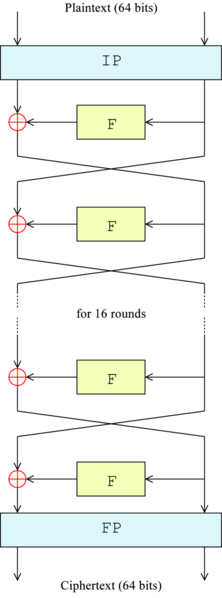
\includegraphics[scale=.7, angle=90]{informatika/algoritmy_a_ds/obrazky/DES-main-network.png}
      \caption{Struktura hlavní sítě algoritmu DES (zdroj: Wikipedie)}
    \end{center}
  \end{figure}

  \paragraph{Analýza:}
  \begin{pitemize}
    \item velká slabina je 64-bitový klíč (navíc efektivně pouze 56-bitový).
    Prolomen za méně než 24 hodin.
    \item úvodní permutace nemá prakticky žádný vliv
    \item existence slabých $(\mathbf{E}(K)=\mathbf{D}(K))$ a poloslabých
    $(\mathbf{E}(K_1)\mathbf{E}(K_2)=Id.)$ klíčů
    \item komplementárnost $C=\mathbf{E}(K,P)\Leftrightarrow\lnot C= \lnot
    \mathbf{E} (\lnot K,\lnot P)$
  \end{pitemize}
\end{obecne}

\begin{obecne}{Blowfish}
  \begin{pitemize}
    \item nástupce systému DES, 
    \item opět Feistelova šifra, délka bloku je 64 bitů, proměnná délka klíče až 448 bitů
    \item algoritmus provádí 16 cyklů nad vstupem délky 64-bitů
  \end{pitemize}
\end{obecne}

\begin{obecne}{IDEA}
  \begin{pitemize}
    \item z roku 1991, vyšel pod názvem IPES. 
    \item IDEA (International Data Encryption Algorithm)
    \item bloková šifra s délkou bloku 64-bitů a délkou klíče 128-bitu
    \item algoritmus je patentován 
    \item zajímavé je že pokud bychom algoritmus upravili tak, že bychom všechny řetězce
    se kterými pracuje zvětšili na dvojnásobek, tak dojde ke ztrátě bezpečnosti.
    \item algoritmus je považován za bezpečný.
  \end{pitemize}
\end{obecne}

\begin{obecne}{RC5}
  \begin{pitemize}
    \item z roku 1994 od R. Rivesta
    \item používá rotace závislé na datech.
    \item algoritmus umožňuje nastavit spoustu parametrů:
    \begin{pitemize}
      \item délka šifrovacího klíče (0\dots255 bytů)
      \item počet kol šifrovacího procesu (0\dots255)
      \item z hodnot 16, 32, 64, ale i vyšších lze zvolit délku slova, algoritmus
      zpracovává bloky o délce dvojnásobku slova
    \end{pitemize}
  \end{pitemize}

\end{obecne}

\begin{obecne}{Kryptosystém Rijndael}
  \begin{pitemize}
    \item produkční bloková šifra
    \item proměnná délka bloku~-- 16, 24 nebo 32 bajtů
    \item proměnná délka klíče~-- 128, 192 nebo 256 bitů
  \end{pitemize}

  \paragraph{Analýza:} Po rozsáhlé analýze nenalezena žádná slabina a tak
  zvolen jako nový standard AES.
\end{obecne}

\begin{obecne}{RC4}
  \begin{pitemize}
    \item proudová šifra od R. Rivesta
    \item jednoduchý a rychlý algoritmus 

    \paragraph{Analýza:} Zatím není známý žádný způsob útoku $\Rightarrow$
    algoritmus považován za bezpečný.
  \end{pitemize}
\end{obecne}

\begin{obecne}{FISH}
  \begin{pitemize}
    \item proudová šifra založena na Fibonacciho generátoru pseudonáhodných čísel.
    \item z fibonacciho generátoru se získá posloupnost a šifrovaní se provádí
    například XORováním této posloupnosti s \emph{P}
  \end{pitemize}
\end{obecne}

\begin{obecne}{Asymetrické}
  \begin{pitemize}
    \item šifry s asymetrickým klíčem~-- RSA, DSA (ElGammal)
    \item mnohem pomalejší
    \item není potřeba TTP
    \item pouze jeden klíč tajný, nemusí se měnit tak často
    \item o žádném schématu veřejného klíče nebylo dokázáno, že je bezpečné
  \end{pitemize}
\end{obecne}

\begin{obecne}{RSA}
  Kryptoschéma je založeno na Eulerově formuli: 
  $$a^{\varphi(n)} \equiv 1(mod\ n)$$ 
  kde $\varphi(n)$ je počet čísel z intervalu $1..n$ která jsou s $n$ nesoudělná.

  \paragraph{Šifrování:} Je třeba znát číslo $n$ a malé prvočíslo $e$. Otevřený
  text převedeme do posloupnosti modulo $n$. Každý blok $P_j$ zašifrujeme dle
  vzorce: $$C_j\equiv P_j^e\ (mod\ n)$$ Spojením výsledných bloků vznikne
  zašifrovaný text.

  \paragraph{Dešifrování:} Je třeba znát číslo $n$ a číslo $d$. Každý z bloků
  potom dešifrujeme takto: $$P_j\equiv C_j^d\ (mod\ n)$$ Pro dešifrovací klíč
  $d$ musí platit: $$ed\equiv 1\,(mod\ \varphi(n))$$ Prvočíslo $e$ nesmí dělit
  $\varphi(n)$. $d$ určíme z předchozího vztahu rozšířeným eukleidovým
  algoritmem.

  Veřejný klíč tvoří pár $(n, e)$, soukromý klíč pár $(n, d)$. Číslo $n$ musí být velmi
  velké a nesmí mít malé faktory. Pro reálné použití 100 až 200 bitů. Hranice bezpečnosti
  1024 bitů modulu $n$, rozumné 1500 bitů, lépe 2048 bitů.

  Není známa žádná metoda vedoucí k rozbití algoritmu RSA. 
\end{obecne}

\begin{obecne}{Merkle-Hellman kryptosystém}
  \begin{pitemize}
    \item založen na problému batohu
    \item plaintext je chápán jako posloupnost vah (řešení)
    \item ciphertext je výsledná hmotnost batohu
    \item pro superrostoucí posloupnost je problém řešitelný v lineárním čase
    \item superrostoucí posloupnost je součást soukromého klíče a tak
    dešifrování pomocí ní je zvládnutelné lineárně, kdežto bez ní je to NP-úplný
    problém
    \item systém byl prolomen! Není tedy považován za bezpečný. Útočník je
    schopen získat superrostoucí posloupnost a pomocí ní může dešifrovat
  \end{pitemize}
\end{obecne}

\begin{obecne}{Elgamal kryptosystém}
  Založen na obtížnosti výpočtu diskrétního logaritmu nad kruhem.

  Potřebujeme společný modul $q$ a číslo $g$ co nejvyššího řádu. Každý účastník si zvolí tajný
  klíč $y_i$ a vypočítá veřejný klíč $g^{y_i}$ mod $q$.
  \paragraph{Šifrování:} Nechť uživatel \emph{A} posílá zprávu \emph{P}
  uživateli \emph{B}. Náhodně
  vybere číslo $k$ a vypočítá: $$ g^k \mod q;\ P \otimes{(g^{y_b})}^k \mod q
  $$ obě čísla zašle \emph{B}.

  \paragraph{Dešifrování:} Uživatel \emph{B} vypočítá: $$ {(g^k)}^{y_b} \mod q$$
  a najde inverzní prvek. Z druhého čísla potom snadno získá \emph{P}.

  Systém je považován za bezpečný. Nevýhodou je nutnost generovat náhodné číslo
  $k$ a zdvojnásobení dat během šifrování.
\end{obecne}


\end{document}
